\renewcommand\thesection{A.\arabic{section}}
\renewcommand\thefigure{A-\arabic{figure}}   
\renewcommand\thetable{A-\arabic{table}}   
\renewcommand\theequation{A.\arabic{equation}}   

\chapter{Appendix} 
\label{ch:Appendix}

\section{Extended derivations}
\label{A:derivations}
\subsection[]{Diffusion propabilistic models}
Several derivations have been presented in a short format for better readability.
This section will cover left-out derivations.
For a more detailed explanation \cite{weng2021WhatAreDiffusion, outlier2022DiffusionModelsPaper} is recommended.
For further details, please refer to \cite{sohl-dickstein2015DeepUnsupervisedLearning, ho2020DenoisingDiffusionProbabilistic}.

Derivation to get from \autoref{eqn:vlb} to \autoref{eqn:vlb2}:

Given:

\begin{equation}
    \label{eqn:kl-divergence_appendix}
    KL(p\parallel q) = \int p(x)\cdot log(\frac{p(x)}{q(x)})dx
\end{equation}

and

\begin{equation}
    \label{eqn:simplify1}
	\begin{align}
    p_\theta(x_{1:T}|x_0) &= \frac{p_\theta(x_0|x_{1:T})p_\theta(x_{1:T})}{p_\theta(x_0)} && \textrm{using bayes rule}\\
	&= \frac{p_\theta(x_0,x_{1:T})}{p_\theta(x_{0})} && \textrm{summarize to joint probability}\\
	&= \frac{p_\theta(x_{0:T})}{p_\theta(x_{0})} && \textrm{summarize to joint probability}\\
\end{align}
\end{equation}

Derivation:
\begingroup
\small
\begin{subequations}
	\label{eqn:vlb2_appendix}
	\begin{align}
		-log(p_\theta(x_0)) &\leq -log(p_\theta(x_0)) + KL(q(x_{1:T}|x_0) \parallel p_\theta(x_{1:T}|x_0)) &&\textrm{}\\
		&= -log(p_\theta(x_0)) + log(\frac{q(x_{1:T})|x_0}{p_\theta(x_{1:T}|x_0)}) && \textrm{using \autoref{eqn:kl-divergence_appendix}}\\
		&=-log(p_\theta(x_0)) + log(\frac{q(x_{1:T})|x_0}{\frac{p_\theta(x_{0:T})}{p_\theta(x_{0})}}) && \textrm{using \autoref{eqn:simplify1}}\\
		&= -log(p_\theta(x_0)) + log(\frac{q(x_{1:T})|x_0}{p_\theta(x_{0:T})})+log(p_\theta(x_{0})) && \textrm{Fraction rule}\\
		&= log(\frac{q(x_{1:T}|x_0)}{p_\theta(x_{0:T})})	&& \textrm{canceling out}\\
		\textrm{Let }L_{VLB} &= \mathbb{E}_{q(x_0:T)}\big[log(\frac{q(x_{1:T}|x_0)}{p_\theta(x_{0:T})}) \big] \geq - \mathbb{E}_{q(x_0)}log(p_\theta(x_0))
	\end{align}
\end{subequations}
\endgroup


Derivation to get from \autoref{eqn:vlb2} to \autoref{eqn:vlb3}:
\begingroup
\small
\begin{subequations}
	\label{eqn:vlb3_appendix}
	\begin{align}
	& L_{VLB}=\mathbb{E}_{q\left(\mathbf{x}_{0: T}\right)}\left[\log \frac{q\left(\mathbf{x}_{1: T} \mid \mathbf{x}_0\right)}{p_\theta\left(\mathbf{x}_{0: T}\right)}\right] \\
	& =\mathbb{E}_q\left[\log \frac{\prod_{t=1}^T q\left(\mathbf{x}_t \mid \mathbf{x}_{t-1}\right)}{p_\theta\left(\mathbf{x}_T\right) \prod_{t=1}^T p_\theta\left(\mathbf{x}_{t-1} \mid \mathbf{x}_t\right)}\right] \\
	& =\mathbb{E}_q\left[-\log p_\theta\left(\mathbf{x}_T\right)+\sum_{t=1}^T \log \frac{q\left(\mathbf{x}_t \mid \mathbf{x}_{t-1}\right)}{p_\theta\left(\mathbf{x}_{t-1} \mid \mathbf{x}_t\right)}\right] \\
	& =\mathbb{E}_q\left[-\log p_\theta\left(\mathbf{x}_T\right)+\sum_{t=2}^T \log \frac{q\left(\mathbf{x}_t \mid \mathbf{x}_{t-1}\right)}{p_\theta\left(\mathbf{x}_{t-1} \mid \mathbf{x}_t\right)}+\log \frac{q\left(\mathbf{x}_1 \mid \mathbf{x}_0\right)}{p_\theta\left(\mathbf{x}_0 \mid \mathbf{x}_1\right)}\right] \\
	& =\mathbb{E}_q\left[-\log p_\theta\left(\mathbf{x}_T\right)+\sum_{t=2}^T \log \left(\frac{q\left(\mathbf{x}_{t-1} \mid \mathbf{x}_t, \mathbf{x}_0\right)}{p_\theta\left(\mathbf{x}_{t-1} \mid \mathbf{x}_t\right)} \cdot \frac{q\left(\mathbf{x}_t \mid \mathbf{x}_0\right)}{q\left(\mathbf{x}_{t-1} \mid \mathbf{x}_0\right)}\right)+\log \frac{q\left(\mathbf{x}_1 \mid \mathbf{x}_0\right)}{p_\theta\left(\mathbf{x}_0 \mid \mathbf{x}_1\right)}\right] \\
	& =\mathbb{E}_q\left[-\log p_\theta\left(\mathbf{x}_T\right)+\sum_{t=2}^T \log \frac{q\left(\mathbf{x}_{t-1} \mid \mathbf{x}_t, \mathbf{x}_0\right)}{p_\theta\left(\mathbf{x}_{t-1} \mid \mathbf{x}_t\right)}+\sum_{t=2}^T \log \frac{q\left(\mathbf{x}_t \mid \mathbf{x}_0\right)}{q\left(\mathbf{x}_{t-1} \mid \mathbf{x}_0\right)}+\log \frac{q\left(\mathbf{x}_1 \mid \mathbf{x}_0\right)}{p_\theta\left(\mathbf{x}_0 \mid \mathbf{x}_1\right)}\right] \\
	& =\mathbb{E}_q\left[-\log p_\theta\left(\mathbf{x}_T\right)+\sum_{t=2}^T \log \frac{q\left(\mathbf{x}_{t-1} \mid \mathbf{x}_t, \mathbf{x}_0\right)}{p_\theta\left(\mathbf{x}_{t-1} \mid \mathbf{x}_t\right)}+\log \frac{q\left(\mathbf{x}_T \mid \mathbf{x}_0\right)}{q\left(\mathbf{x}_1 \mid \mathbf{x}_0\right)}+\log \frac{q\left(\mathbf{x}_1 \mid \mathbf{x}_0\right)}{p_\theta\left(\mathbf{x}_0 \mid \mathbf{x}_1\right)}\right] \\
	& =\mathbb{E}_q\left[\log \frac{q\left(\mathbf{x}_T \mid \mathbf{x}_0\right)}{p_\theta\left(\mathbf{x}_T\right)}+\sum_{t=2}^T \log \frac{q\left(\mathbf{x}_{t-1} \mid \mathbf{x}_t, \mathbf{x}_0\right)}{p_\theta\left(\mathbf{x}_{t-1} \mid \mathbf{x}_t\right)}-\log p_\theta\left(\mathbf{x}_0 \mid \mathbf{x}_1\right)\right] \\
	& =\mathbb{E}_q[\underbrace{D_{\mathrm{KL}}\left(q\left(\mathbf{x}_T \mid \mathbf{x}_0\right) \| p_\theta\left(\mathbf{x}_T\right)\right)}_{L_T}+\sum_{t=2}^T \underbrace{D_{\mathrm{KL}}\left(q\left(\mathbf{x}_{t-1} \mid \mathbf{x}_t, \mathbf{x}_0\right) \| p_\theta\left(\mathbf{x}_{t-1} \mid \mathbf{x}_t\right)\right)}_{L_{t-1}}-\underbrace{\log p_\theta\left(\mathbf{x}_0 \mid \mathbf{x}_1\right)}_{L_0}]
	\end{align}
\end{subequations}
\endgroup

\newpage
\section{Activity diagrams}
\label{A:activity_diagrams}

The following section will display the procedures of different scripts.
Firstly, the scripts' most important processes are displayed as implemented by \cite{kotelnikov2022TabDDPMModellingTabular}. 
The process of the scripts with the implemented changes are displayed afterward.
\subsection[]{Original Implementation}
\begin{figure}[!b]
	\centering
	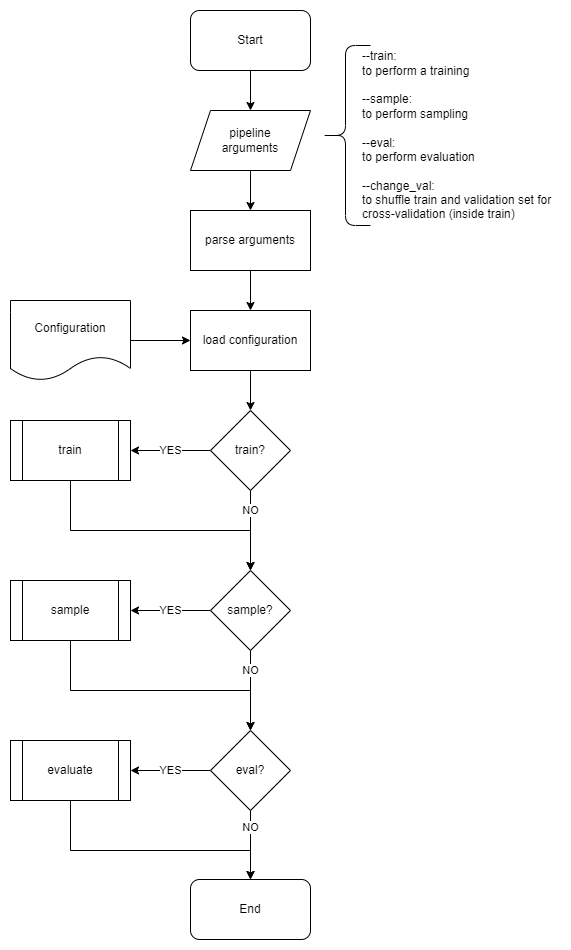
\includegraphics[width=\textwidth, height=0.7\textheight, keepaspectratio]{images/pipeline-ORIGINAL.png}
	\caption[Pipeline Script]{simplified visualization of the pipeline\_\*.py script}
\end{figure}
\begin{figure}
	\centering
	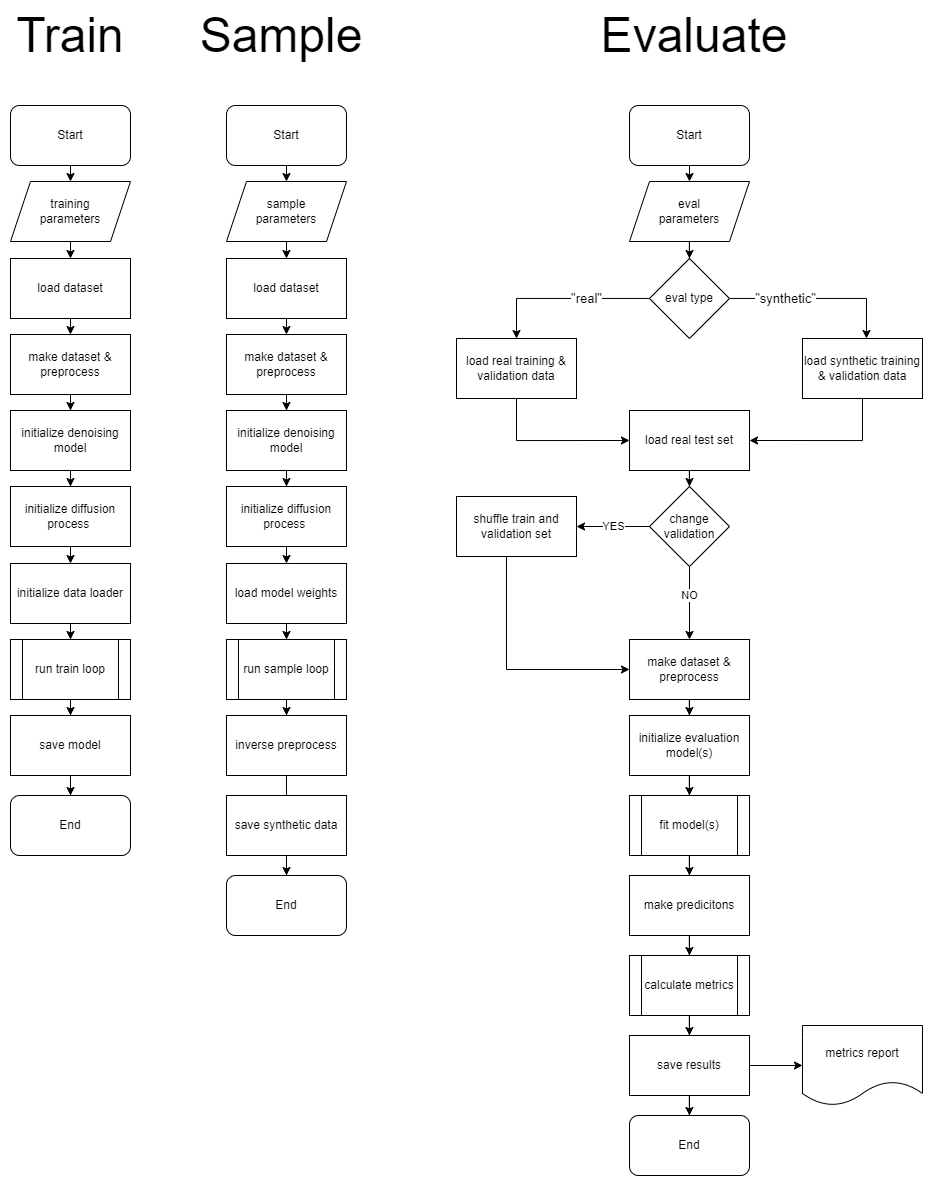
\includegraphics[width=\textwidth]{images/train-sample-eval.png}
	\caption[Train, Sample, Evaluation Script]{simplified visualization of the train.py, sample.py and eval\_[catboost|mlp|simple].py scripts}
	\label{fig:a_original_train_sample_eval}
\end{figure}
\begin{landscape}
\begin{figure}
	\centering
	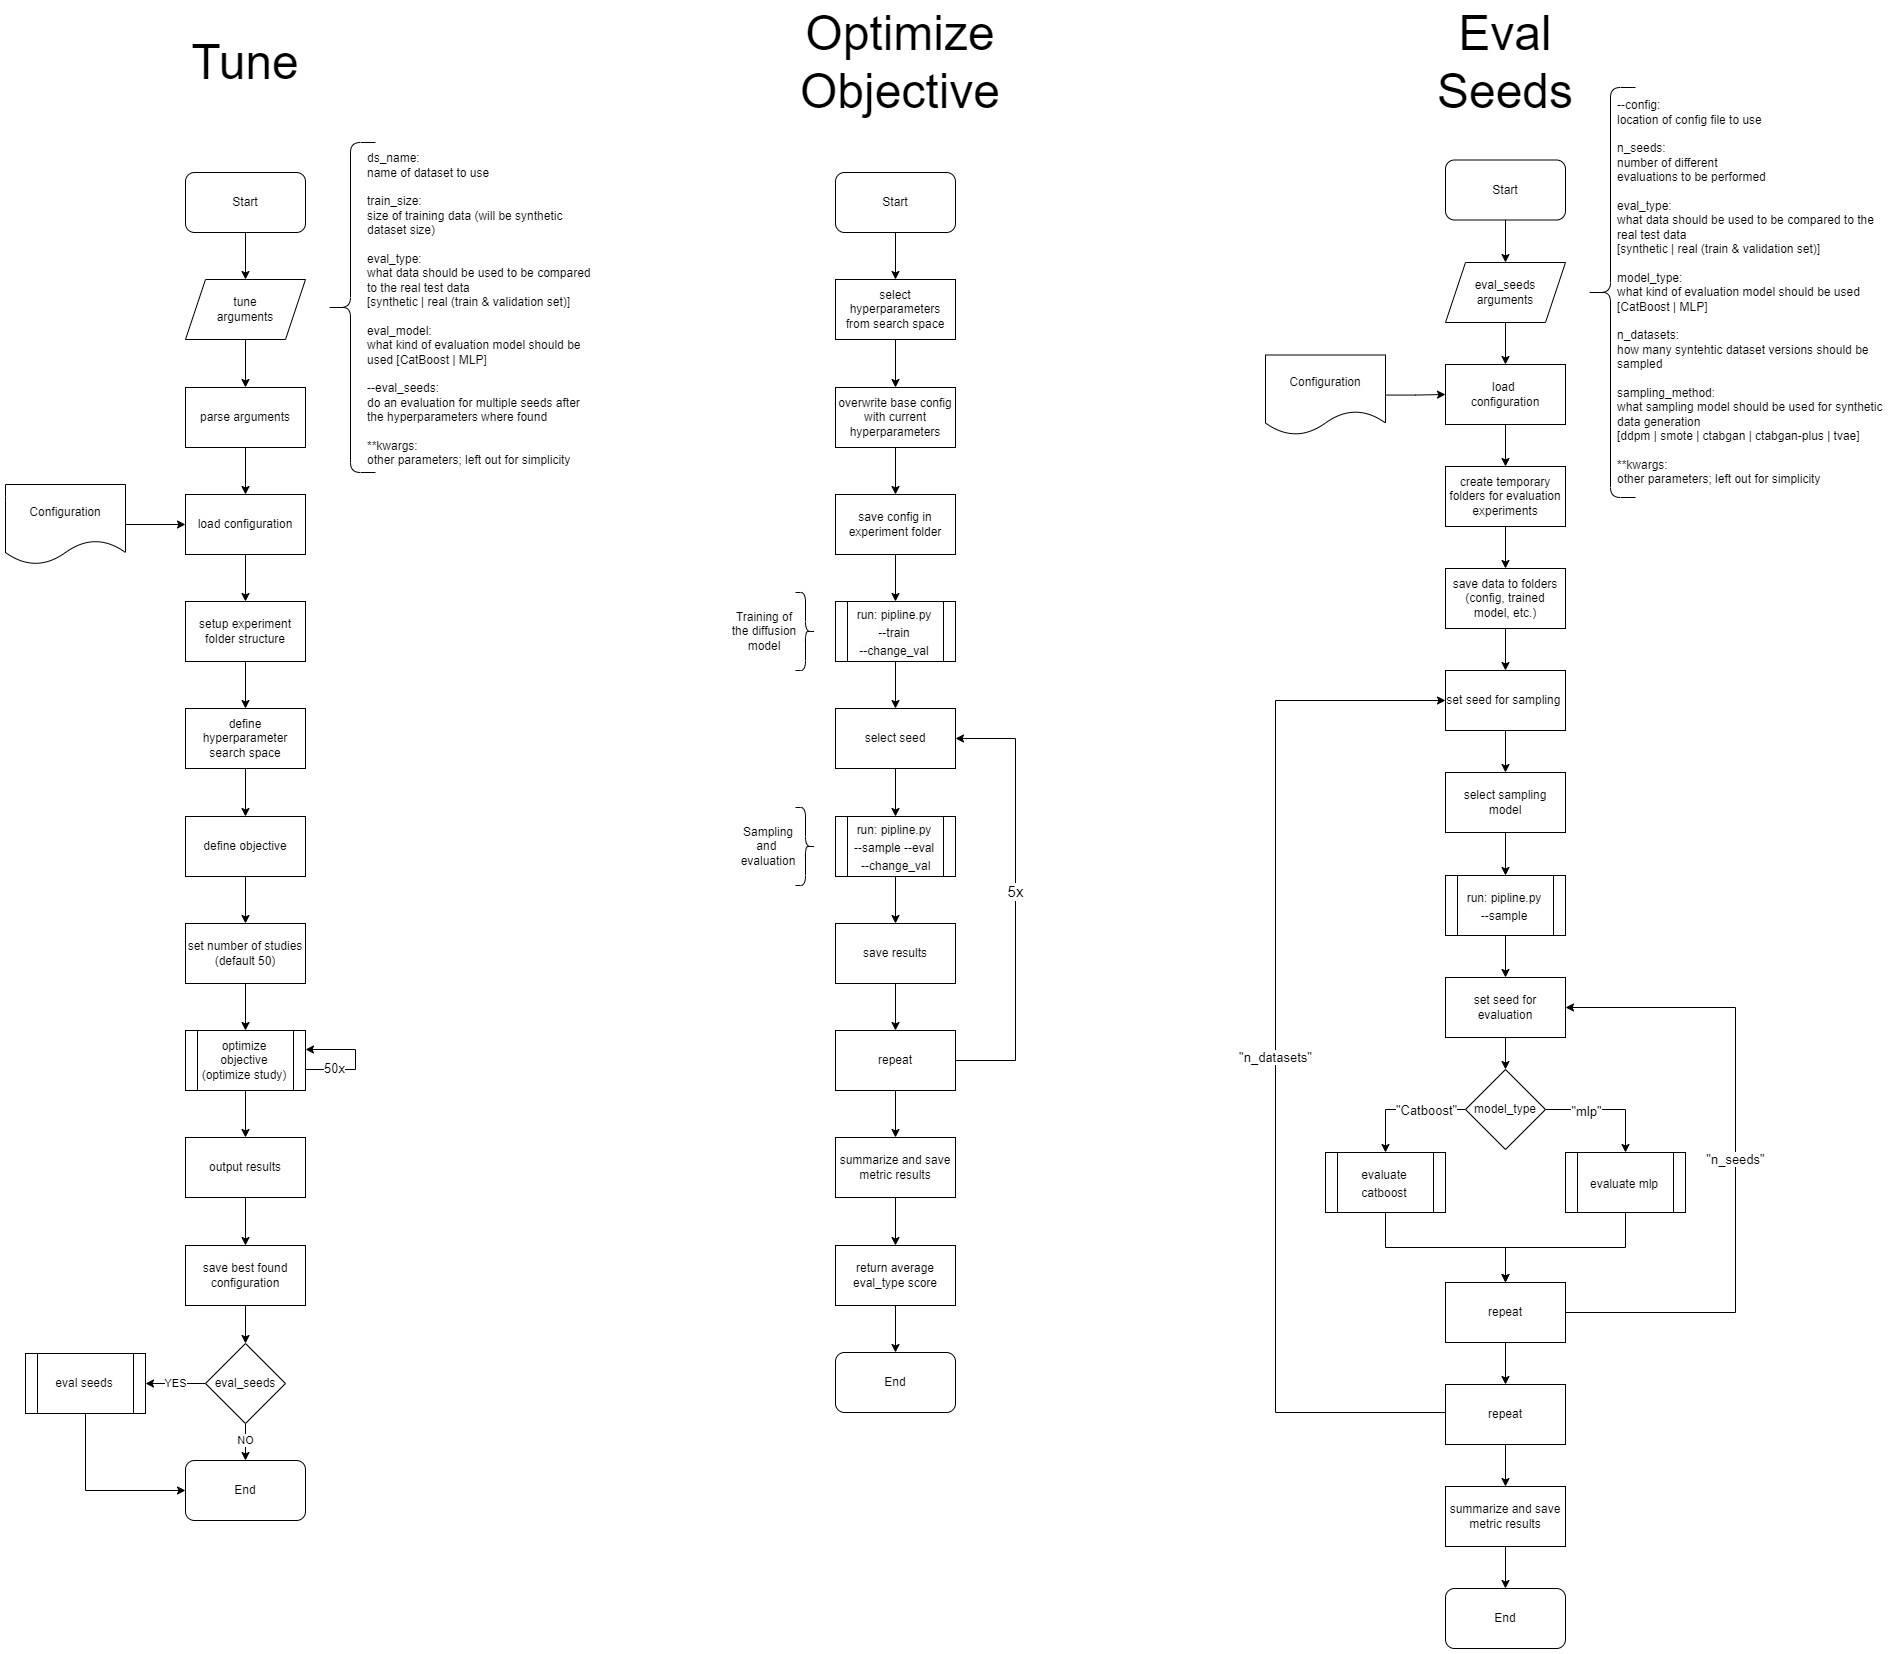
\includegraphics[height=\textheight,width=\linewidth,keepaspectratio]{images/tune_eval_seeds-ORIGINAL.png}
	\caption[Tuning Script]{simplified visualization of the tune\_*.py scripts and the eval\_seeds.py}
\end{figure}
\end{landscape}

\subsection[]{Changed Implementation}
Several changes have been made to the different scripts.
The following figures will display the most important changes, highlighted in green.
Please note that not all changes to the original implementation can be included, and minor modifications or bug fixes are not displayed.

\begin{figure}
	\centering
	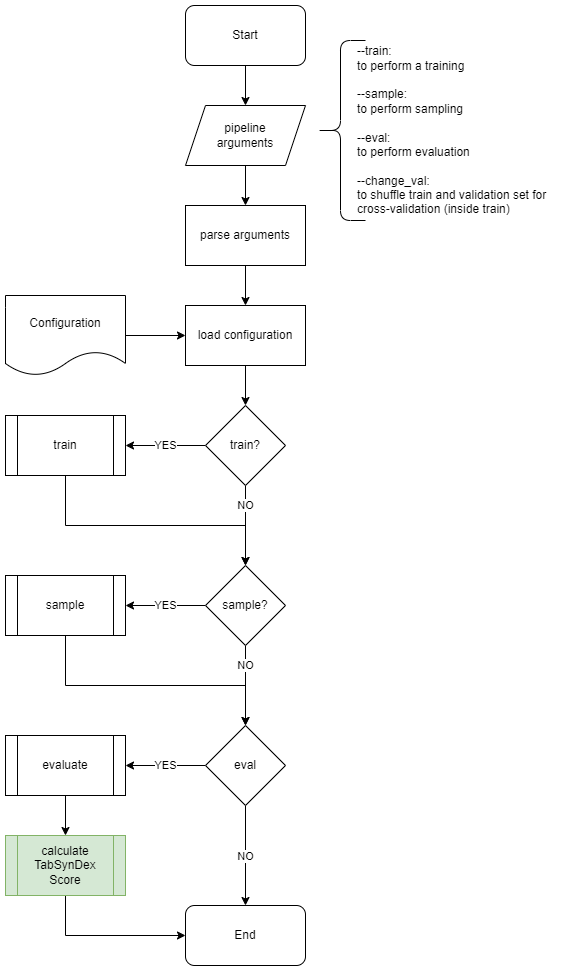
\includegraphics[width=\textwidth, height=\textheight, keepaspectratio]{images/pipeline-CHANGED.png}
	\caption[Pipeline Script Changes]{simplified visualization of the changed pipeline\_\*.py script}
	\label{fig:a_pipeline_changed}.
\end{figure}
The basic pipeline script hardly changed.
However, the individual components did change and are displayed in \autoref{fig:a_train_sample_eval}.
The previous evaluation part in \autoref{fig:a_original_train_sample_eval} is unchanged.
Instead,  \autoref{fig:a_train_sample_eval} displays only the new similarity evaluation script, which is
executed after the previous evaluation script (compare \autoref{fig:a_pipeline_changed}).
\begin{figure}
	\centering
	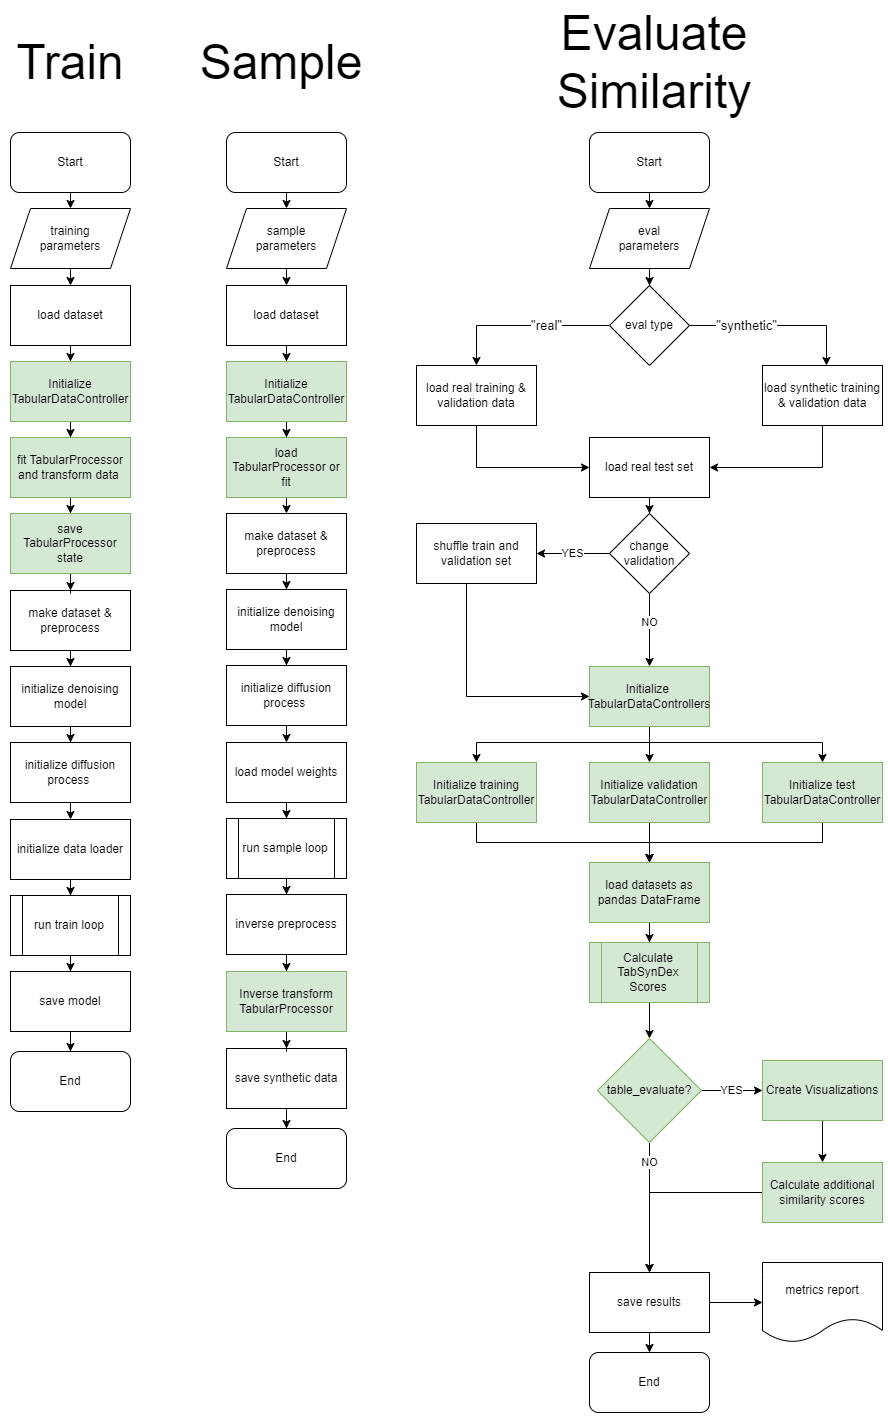
\includegraphics[width=\textwidth]{images/train-sample-eval-Changed.png}
	\caption[Train, Sample, Evaluation Script Changes]{simplified visualization of the train.py, sample.py and eval\_[catboost|mlp|simple].py scripts}
	\label{fig:a_train_sample_eval}
\end{figure}
\begin{landscape}
	\begin{figure}
		\centering
		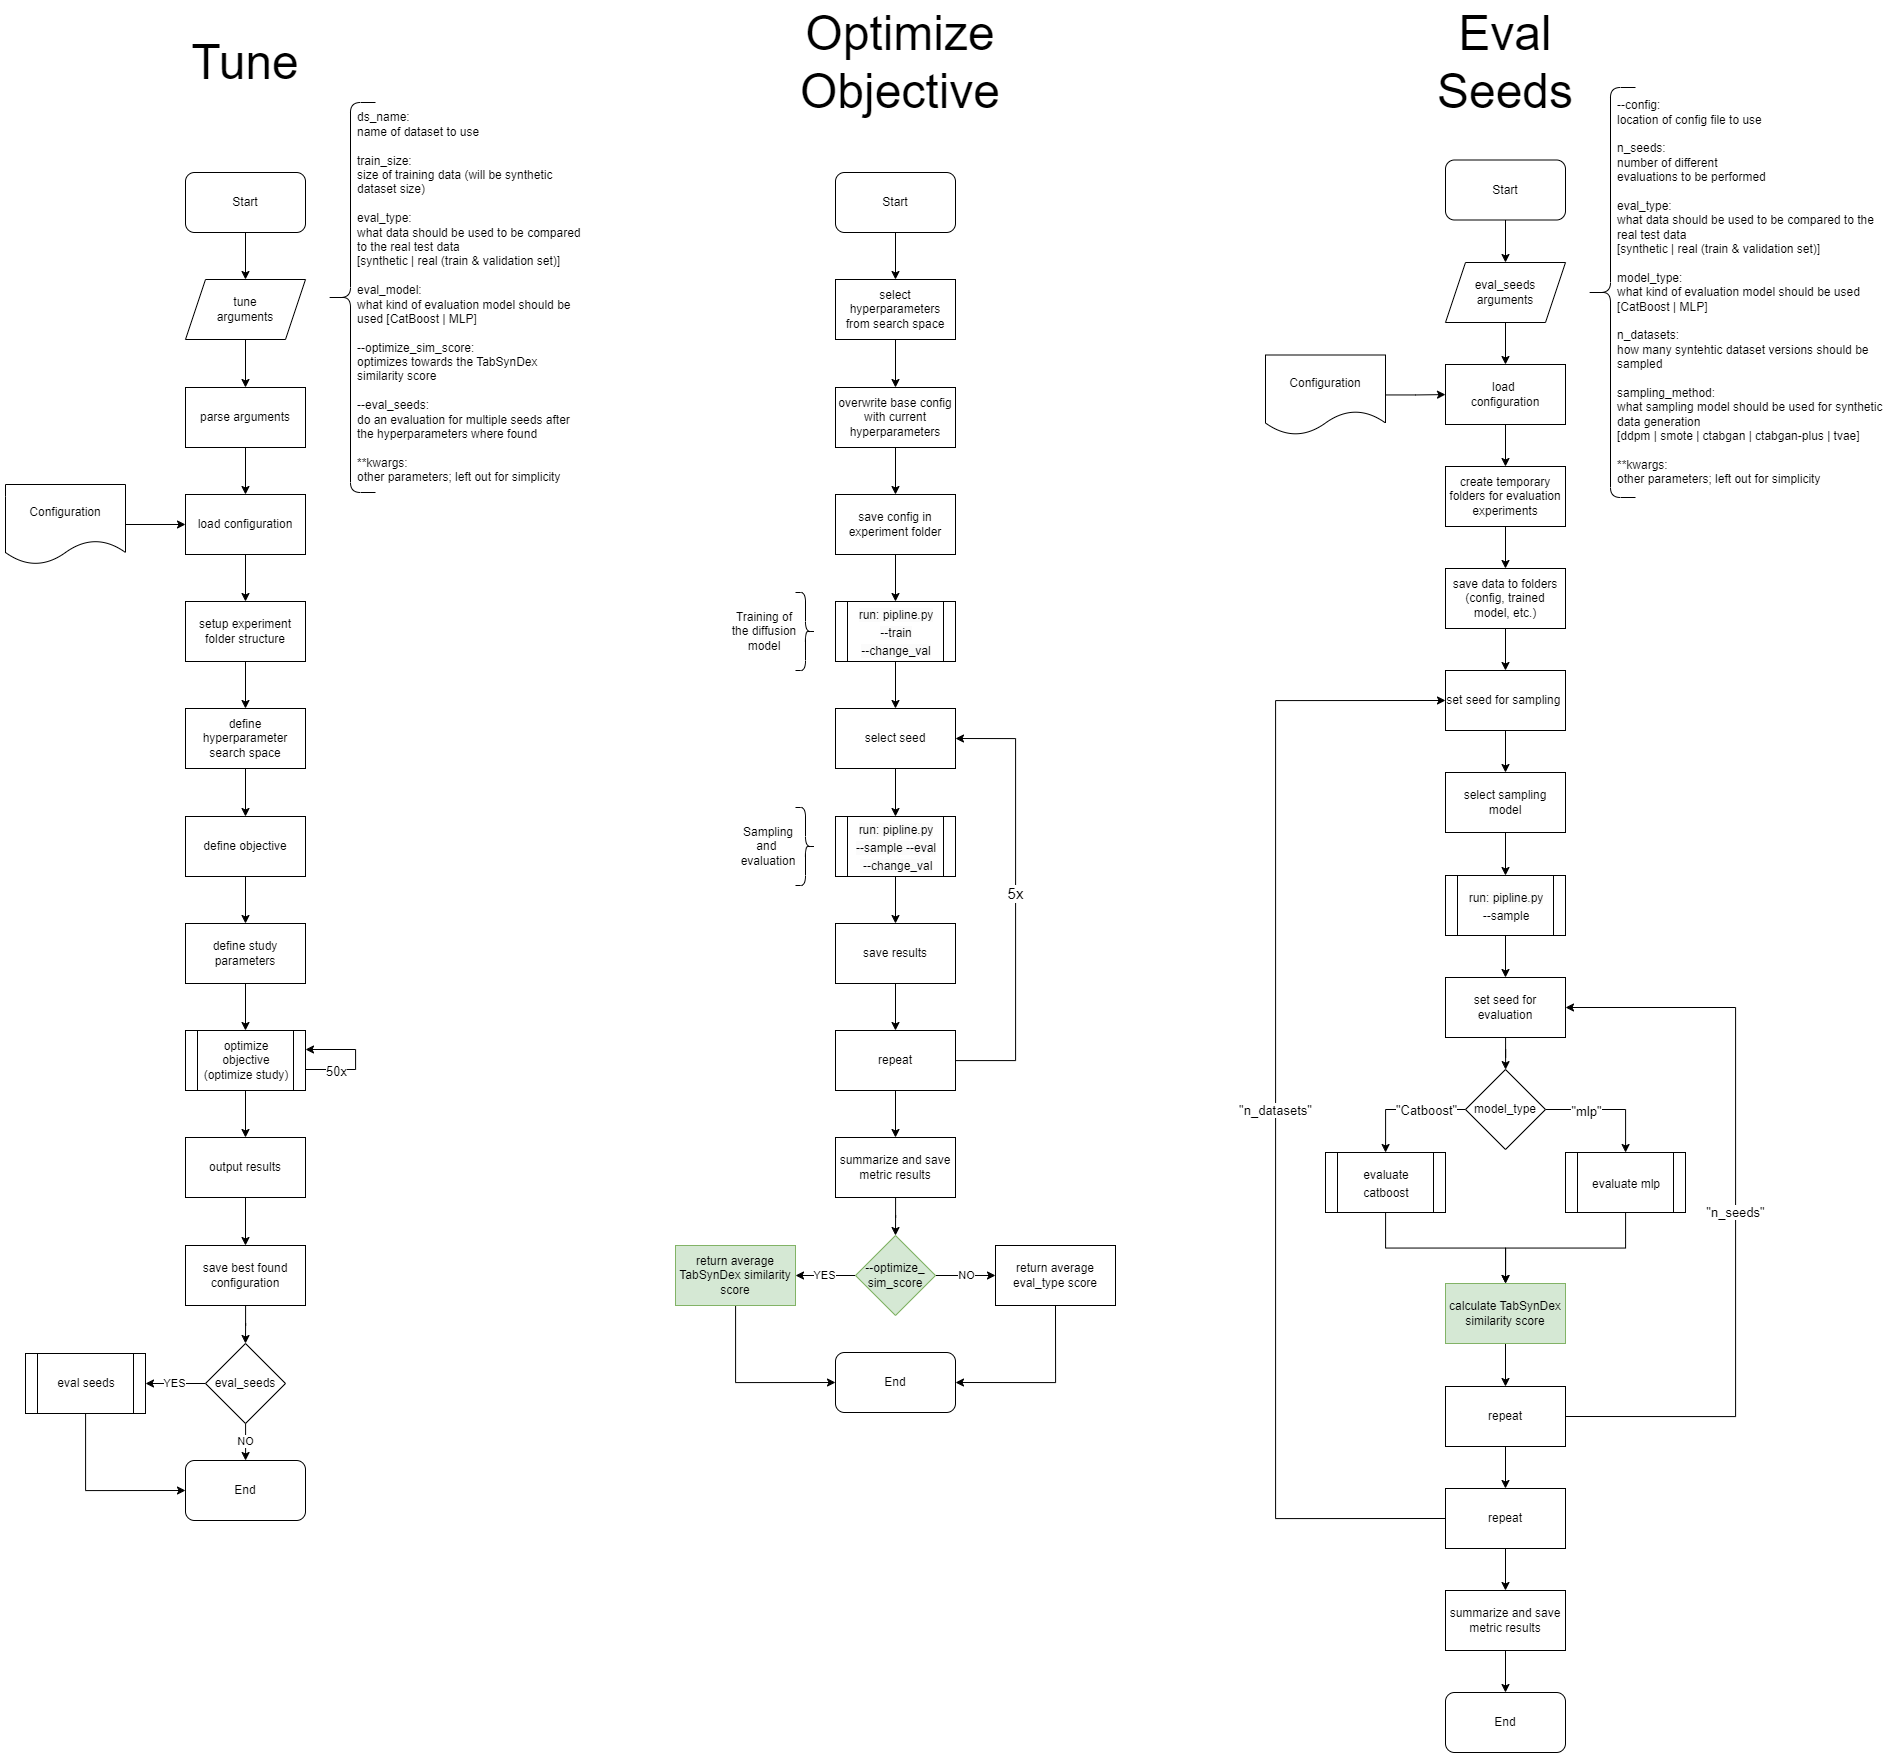
\includegraphics[height=\textheight,width=\linewidth,keepaspectratio]{images/tune_eval_seeds-CHANGED.png}
		\caption[Tuning Script Changes]{simplified visualization of the changed tune\_*.py scripts and the changed eval\_seeds.py}
	\end{figure}
\end{landscape}





\section{Visual Results}
\label{A:Visual_results}
\subsection[]{Correlation Difference Matrix}
\label{A:corr_matrix}

\begin{figure}[h]
	\centering
	\begin{subfigure}{0.3\textwidth}
		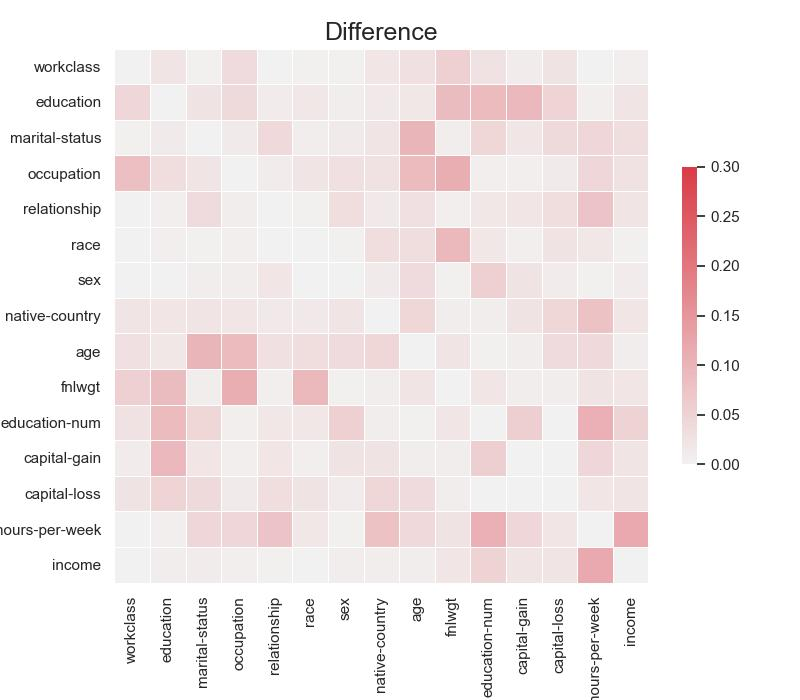
\includegraphics[width=\textwidth]{images/correlation_difference/ctabgan_simTune.jpg}
		\caption{CTABGAN$^s$}
	\end{subfigure}
	\begin{subfigure}{0.3\textwidth}
		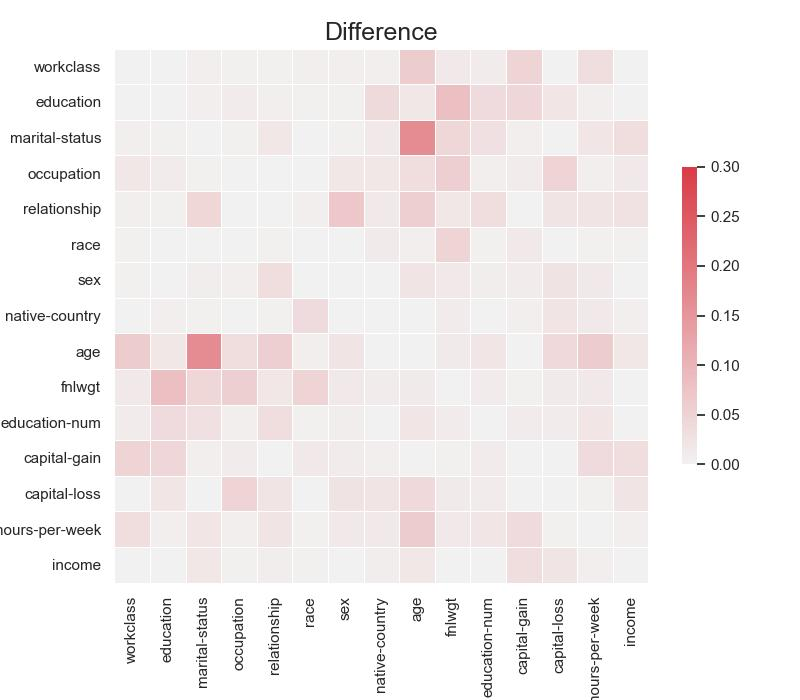
\includegraphics[width=\textwidth]{images/correlation_difference/ctabgan+_simTune.jpg}
		\caption{CTABGAN+$^s$}
	\end{subfigure}
    \begin{subfigure}{0.3\textwidth}
        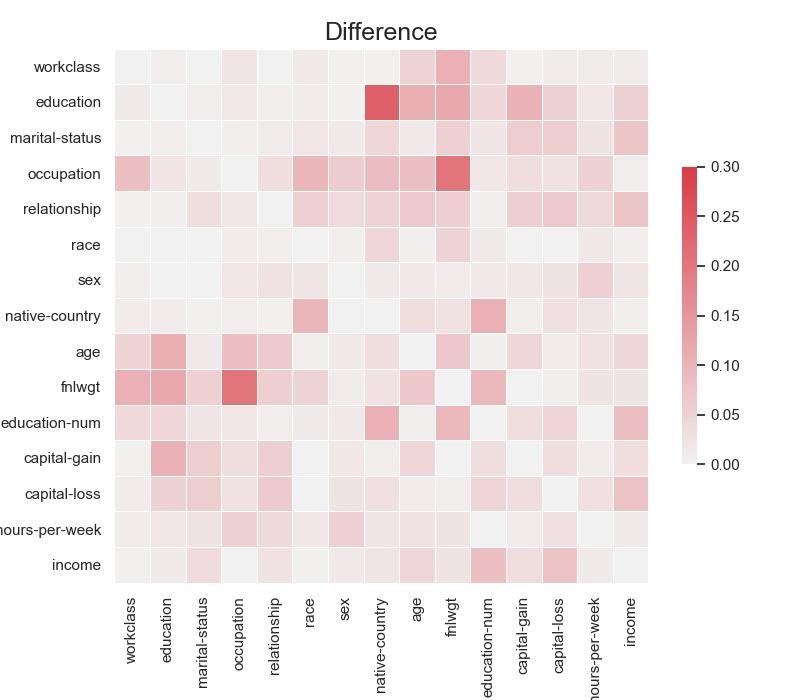
\includegraphics[width=\textwidth]{images/correlation_difference/tvae_simTune.jpg}
        \caption{TVAE$^s$}
    \end{subfigure}
	\begin{subfigure}{0.3\textwidth}
		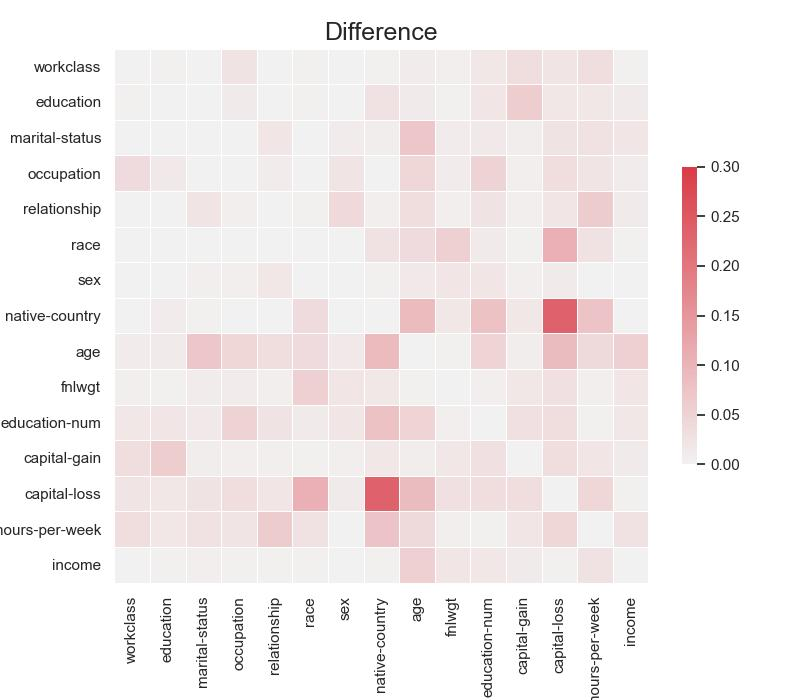
\includegraphics[width=\textwidth]{images/correlation_difference/tab-ddpm-bgm-simTune.jpg}
		\caption{TabDDPM-BGM$^{s}_q$}
	\end{subfigure}
    \begin{subfigure}{0.3\textwidth}
        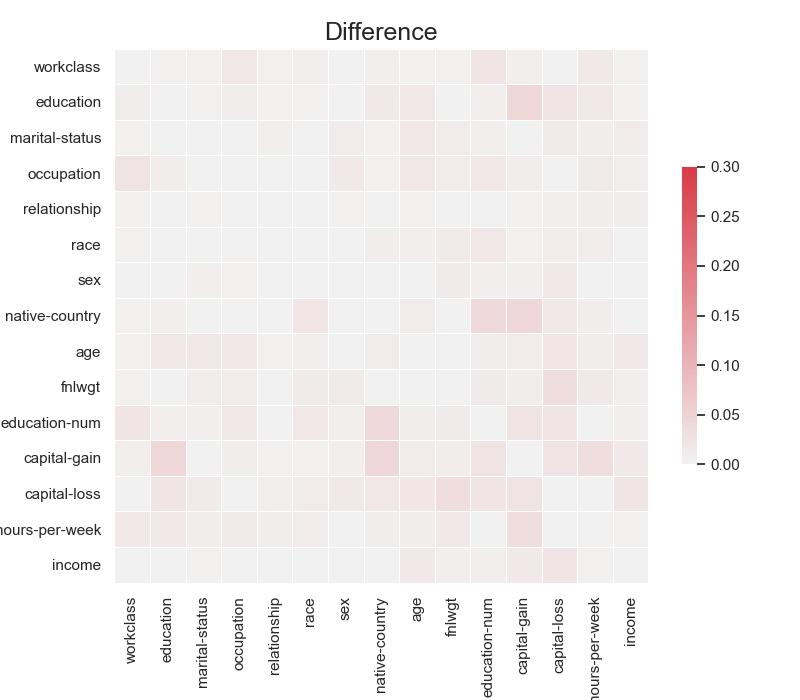
\includegraphics[width=\textwidth]{images/correlation_difference/tab-ddpm-bgm-simTune-minmax.jpg}
        \caption{TabDDPM-BGM$^{s}_m$}
    \end{subfigure}
	\begin{subfigure}{0.3\textwidth}
        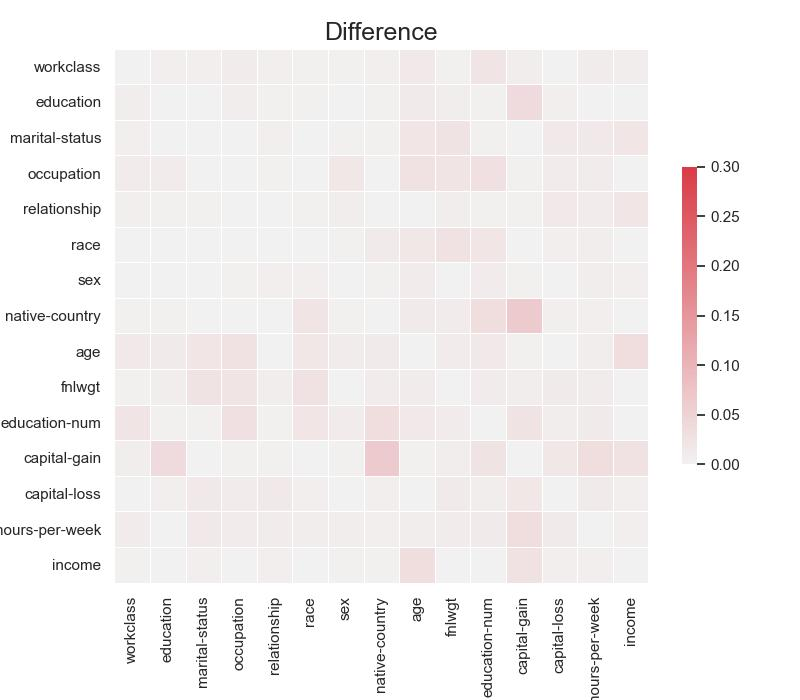
\includegraphics[width=\textwidth]{images/correlation_difference/tab-ddpm-bgm-simTune-none.jpg}
        \caption{TabDDPM-BGM$^{s}_n$}
    \end{subfigure}
	\begin{subfigure}{0.3\textwidth}
		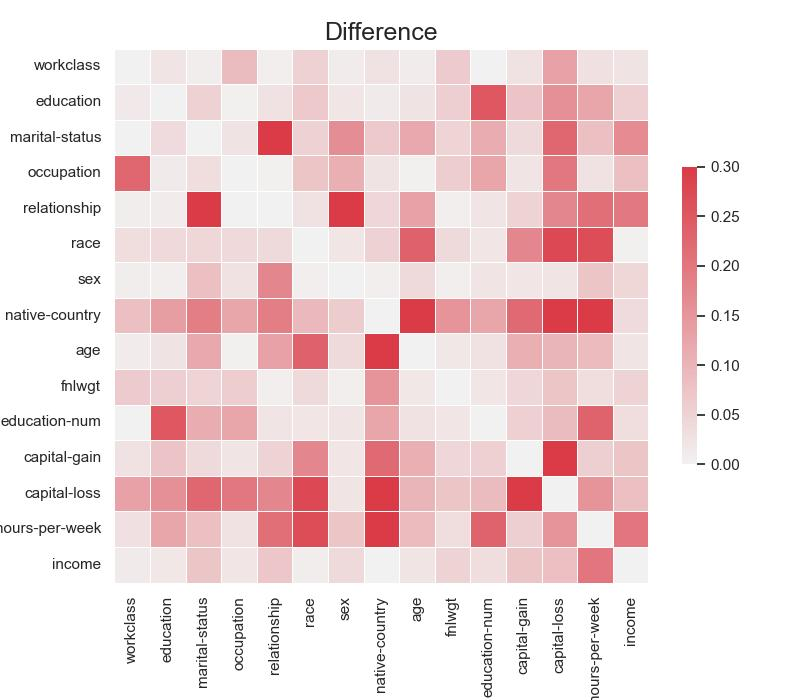
\includegraphics[width=\textwidth]{images/correlation_difference/tab-ddpm-ft-simTune.jpg}
		\caption{TabDDPM-FT$^{s}_q$}
    \end{subfigure}
    \caption{Correlation difference matrix for different model versions}
	\label{fig_a:corr_diff}
\end{figure}

\newpage
\subsection[]{Principle Component Analysis}
\label{A:pca}

\begin{figure}[h]
	\centering
	\begin{subfigure}{0.3\textwidth}
		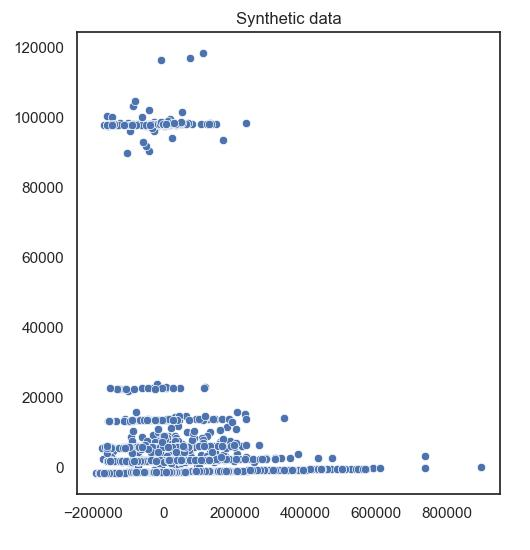
\includegraphics[width=\textwidth]{images/pca/ctabgan_simTune.jpg}
		\caption{CTABGAN$^s$}
	\end{subfigure}
	\begin{subfigure}{0.3\textwidth}
		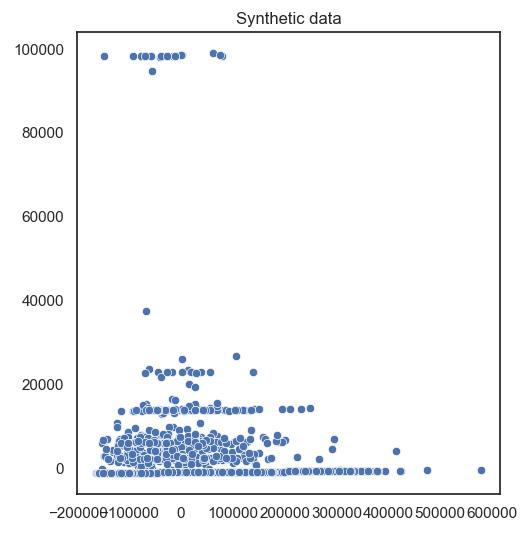
\includegraphics[width=\textwidth]{images/pca/ctabgan+_simTune.jpg}
		\caption{CTABGAN+$^s$}
	\end{subfigure}
    \begin{subfigure}{0.3\textwidth}
        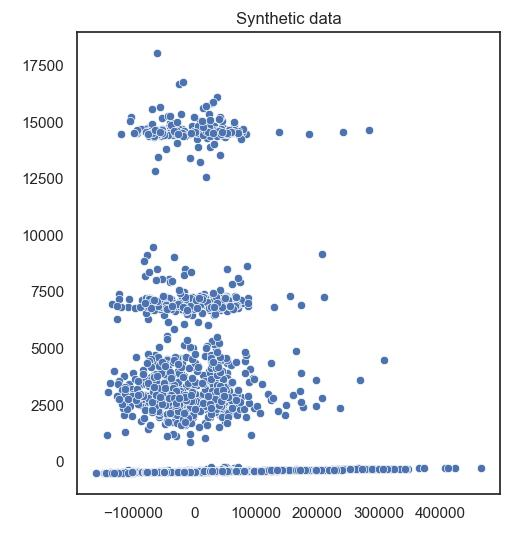
\includegraphics[width=\textwidth]{images/pca/tvae_simTune.jpg}
        \caption{TVAE$^s$}
    \end{subfigure}
	\begin{subfigure}{0.3\textwidth}
		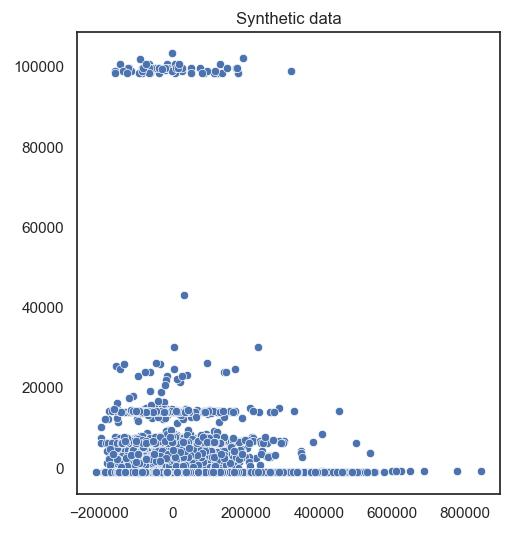
\includegraphics[width=\textwidth]{images/pca/tab-ddpm-bgm-simTune.jpg}
		\caption{TabDDPM-BGM$^{s}_q$}
	\end{subfigure}
	\begin{subfigure}{0.3\textwidth}
		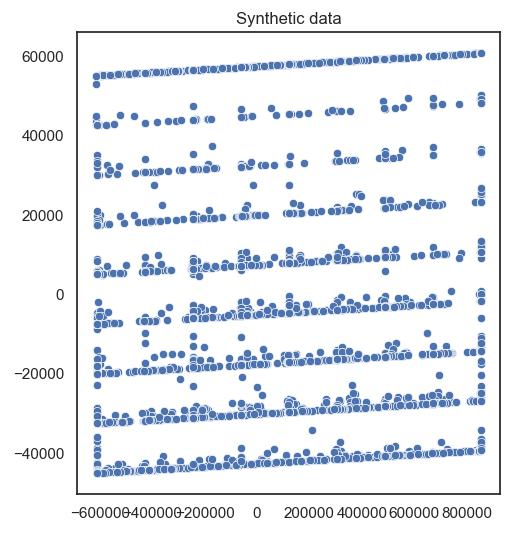
\includegraphics[width=\textwidth]{images/pca/tab-ddpm-ft-simTune.jpg}
		\caption{TabDDPM-FT$^{s}_q$}
    \end{subfigure}
	\begin{subfigure}{0.3\textwidth}
		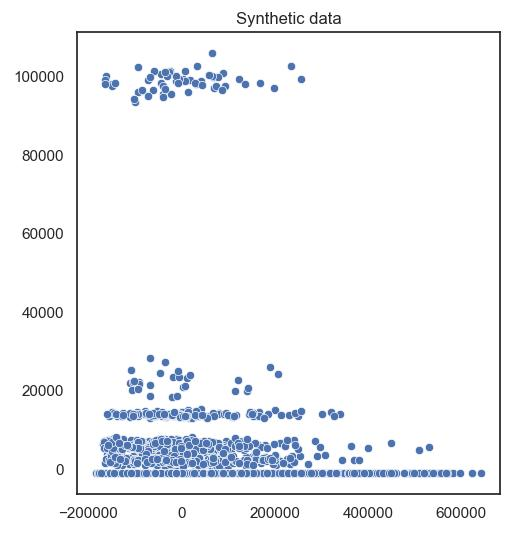
\includegraphics[width=\textwidth]{images/pca/tab-ddpm-bgm-simTune-minmax.jpg}
		\caption{TabDDPM-BGM$^{s}_m$}
		\label{fig_a:pca_TabDDPMBM}
    \end{subfigure}
	\begin{subfigure}{0.3\textwidth}
		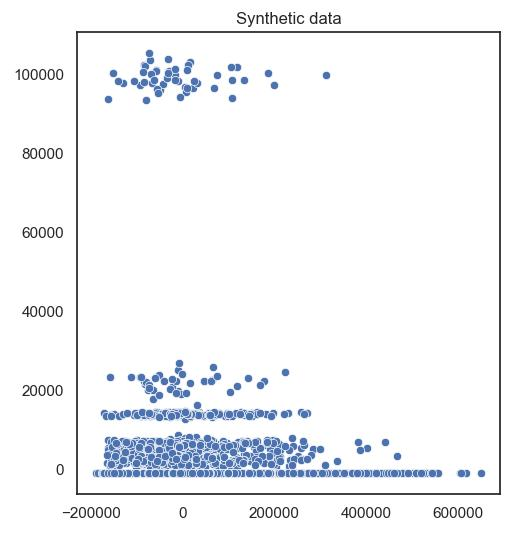
\includegraphics[width=\textwidth]{images/pca/tab-ddpm-bgm-simTune-none.jpg}
		\caption{TabDDPM-BGM$^{s}_n$}
    \end{subfigure}
    \caption[PCA plots Experiment Models]{Principle Component Analysis for different model versions}
    \label{fig_a:pca_diff}
\end{figure}
\newpage

\subsection[]{Distribution Plots}
\label{A:distributions}
\begin{figure}[h]
	\centering
	\begin{subfigure}{0.6\linewidth}
		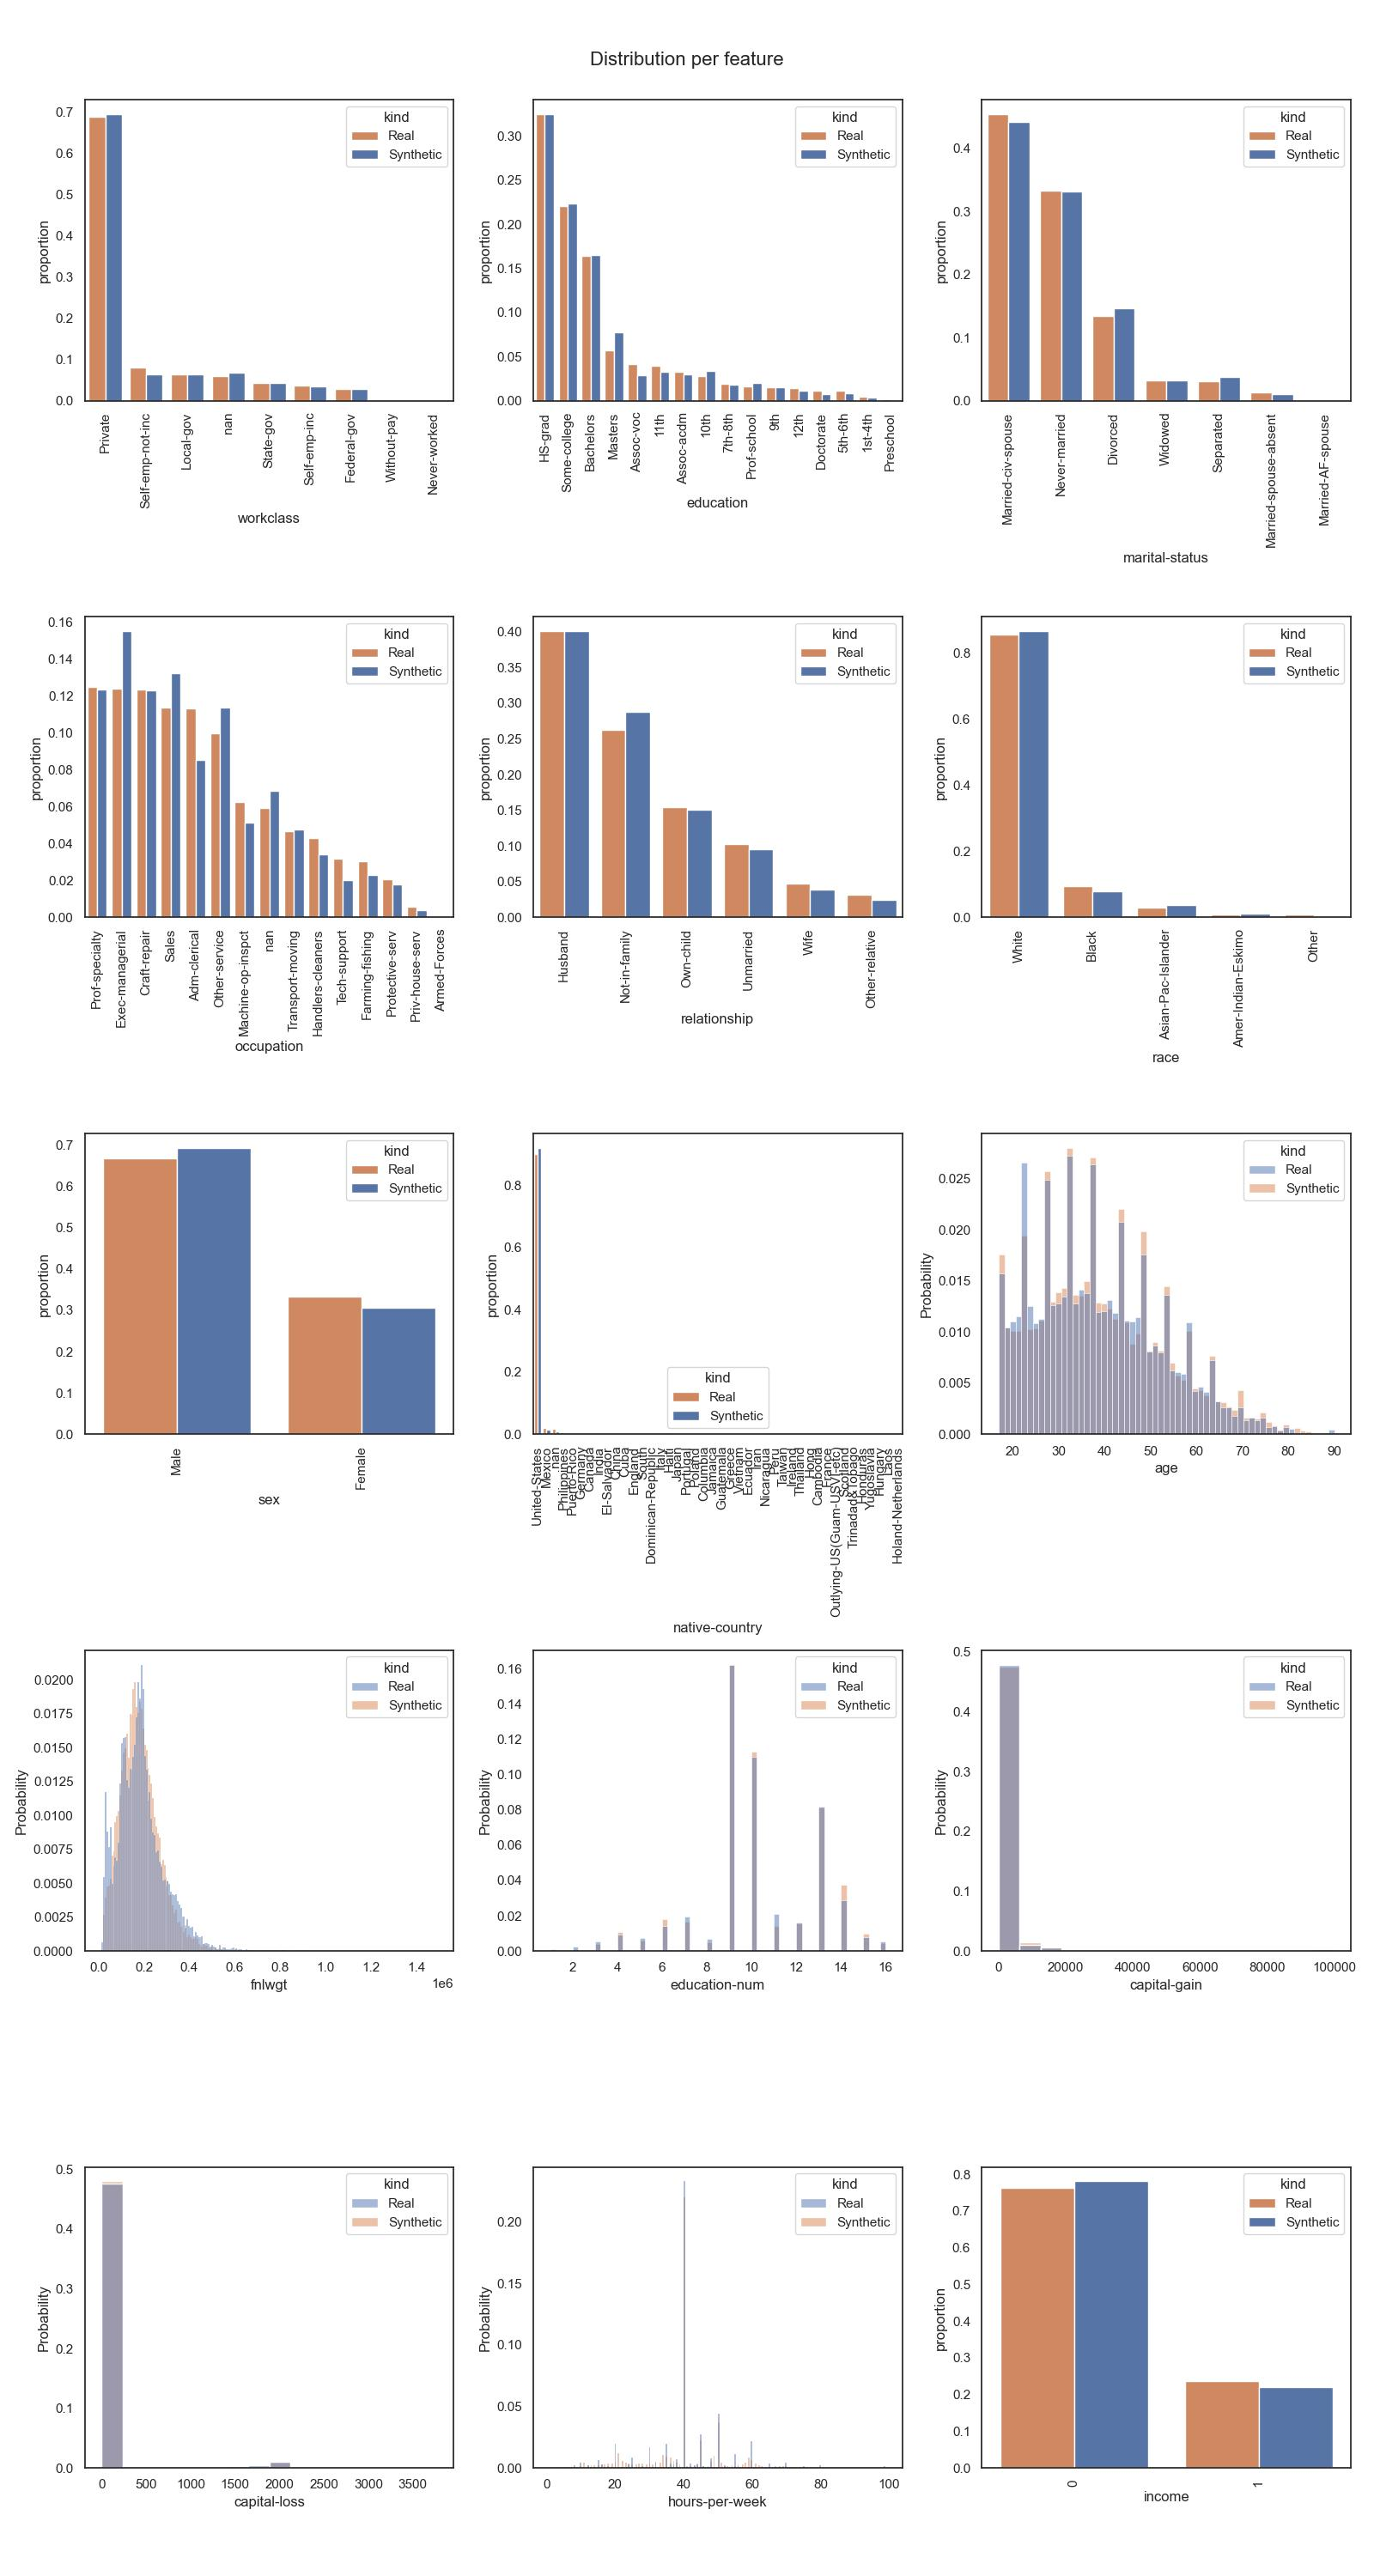
\includegraphics[height=\textheight,width=\linewidth,keepaspectratio]{images/distributions_full/ctabgan+.jpg}
		\caption{CTABGAN+$^{ml}$}
	\end{subfigure}
\end{figure}


\begin{landscape}
	\begin{figure}[h]
		\centering
		\hfill
		\begin{subfigure}{0.3\linewidth}
			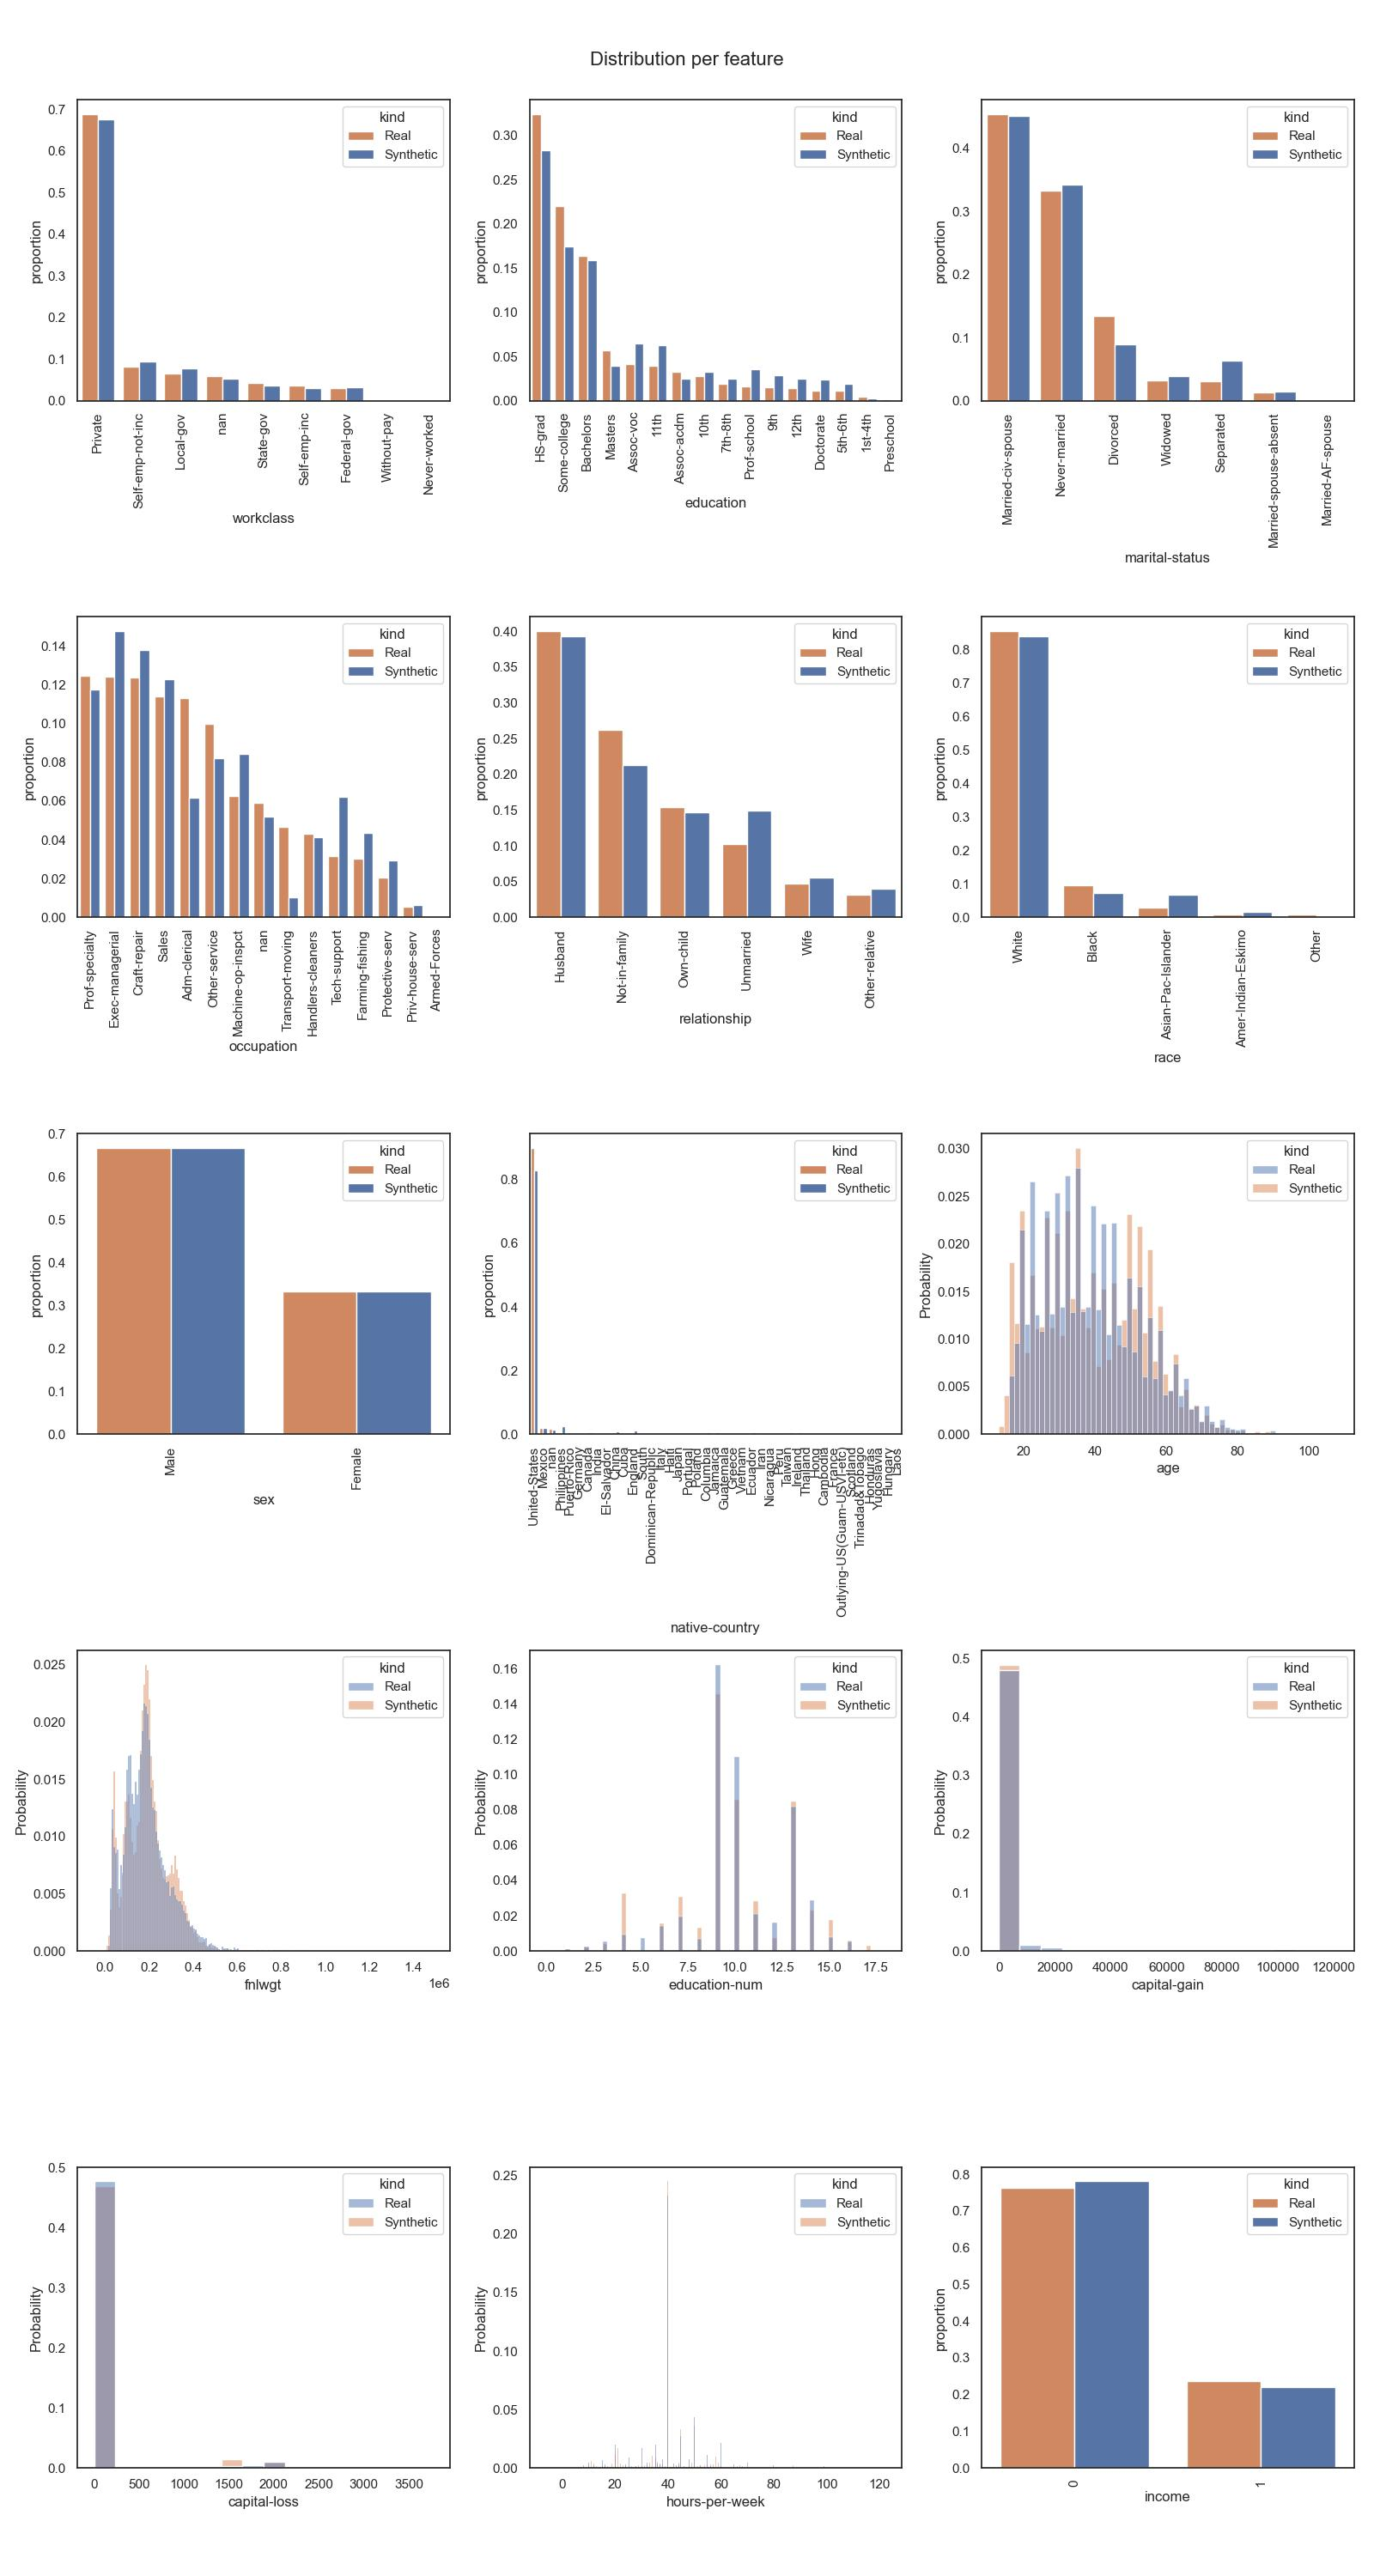
\includegraphics[height=\textheight,width=\linewidth,keepaspectratio]{images/distributions_full/ctabgan.jpg}
			\caption{CTABGAN$^{ml}$}
		\end{subfigure}
		\hfill
		\begin{subfigure}{0.3\linewidth}
			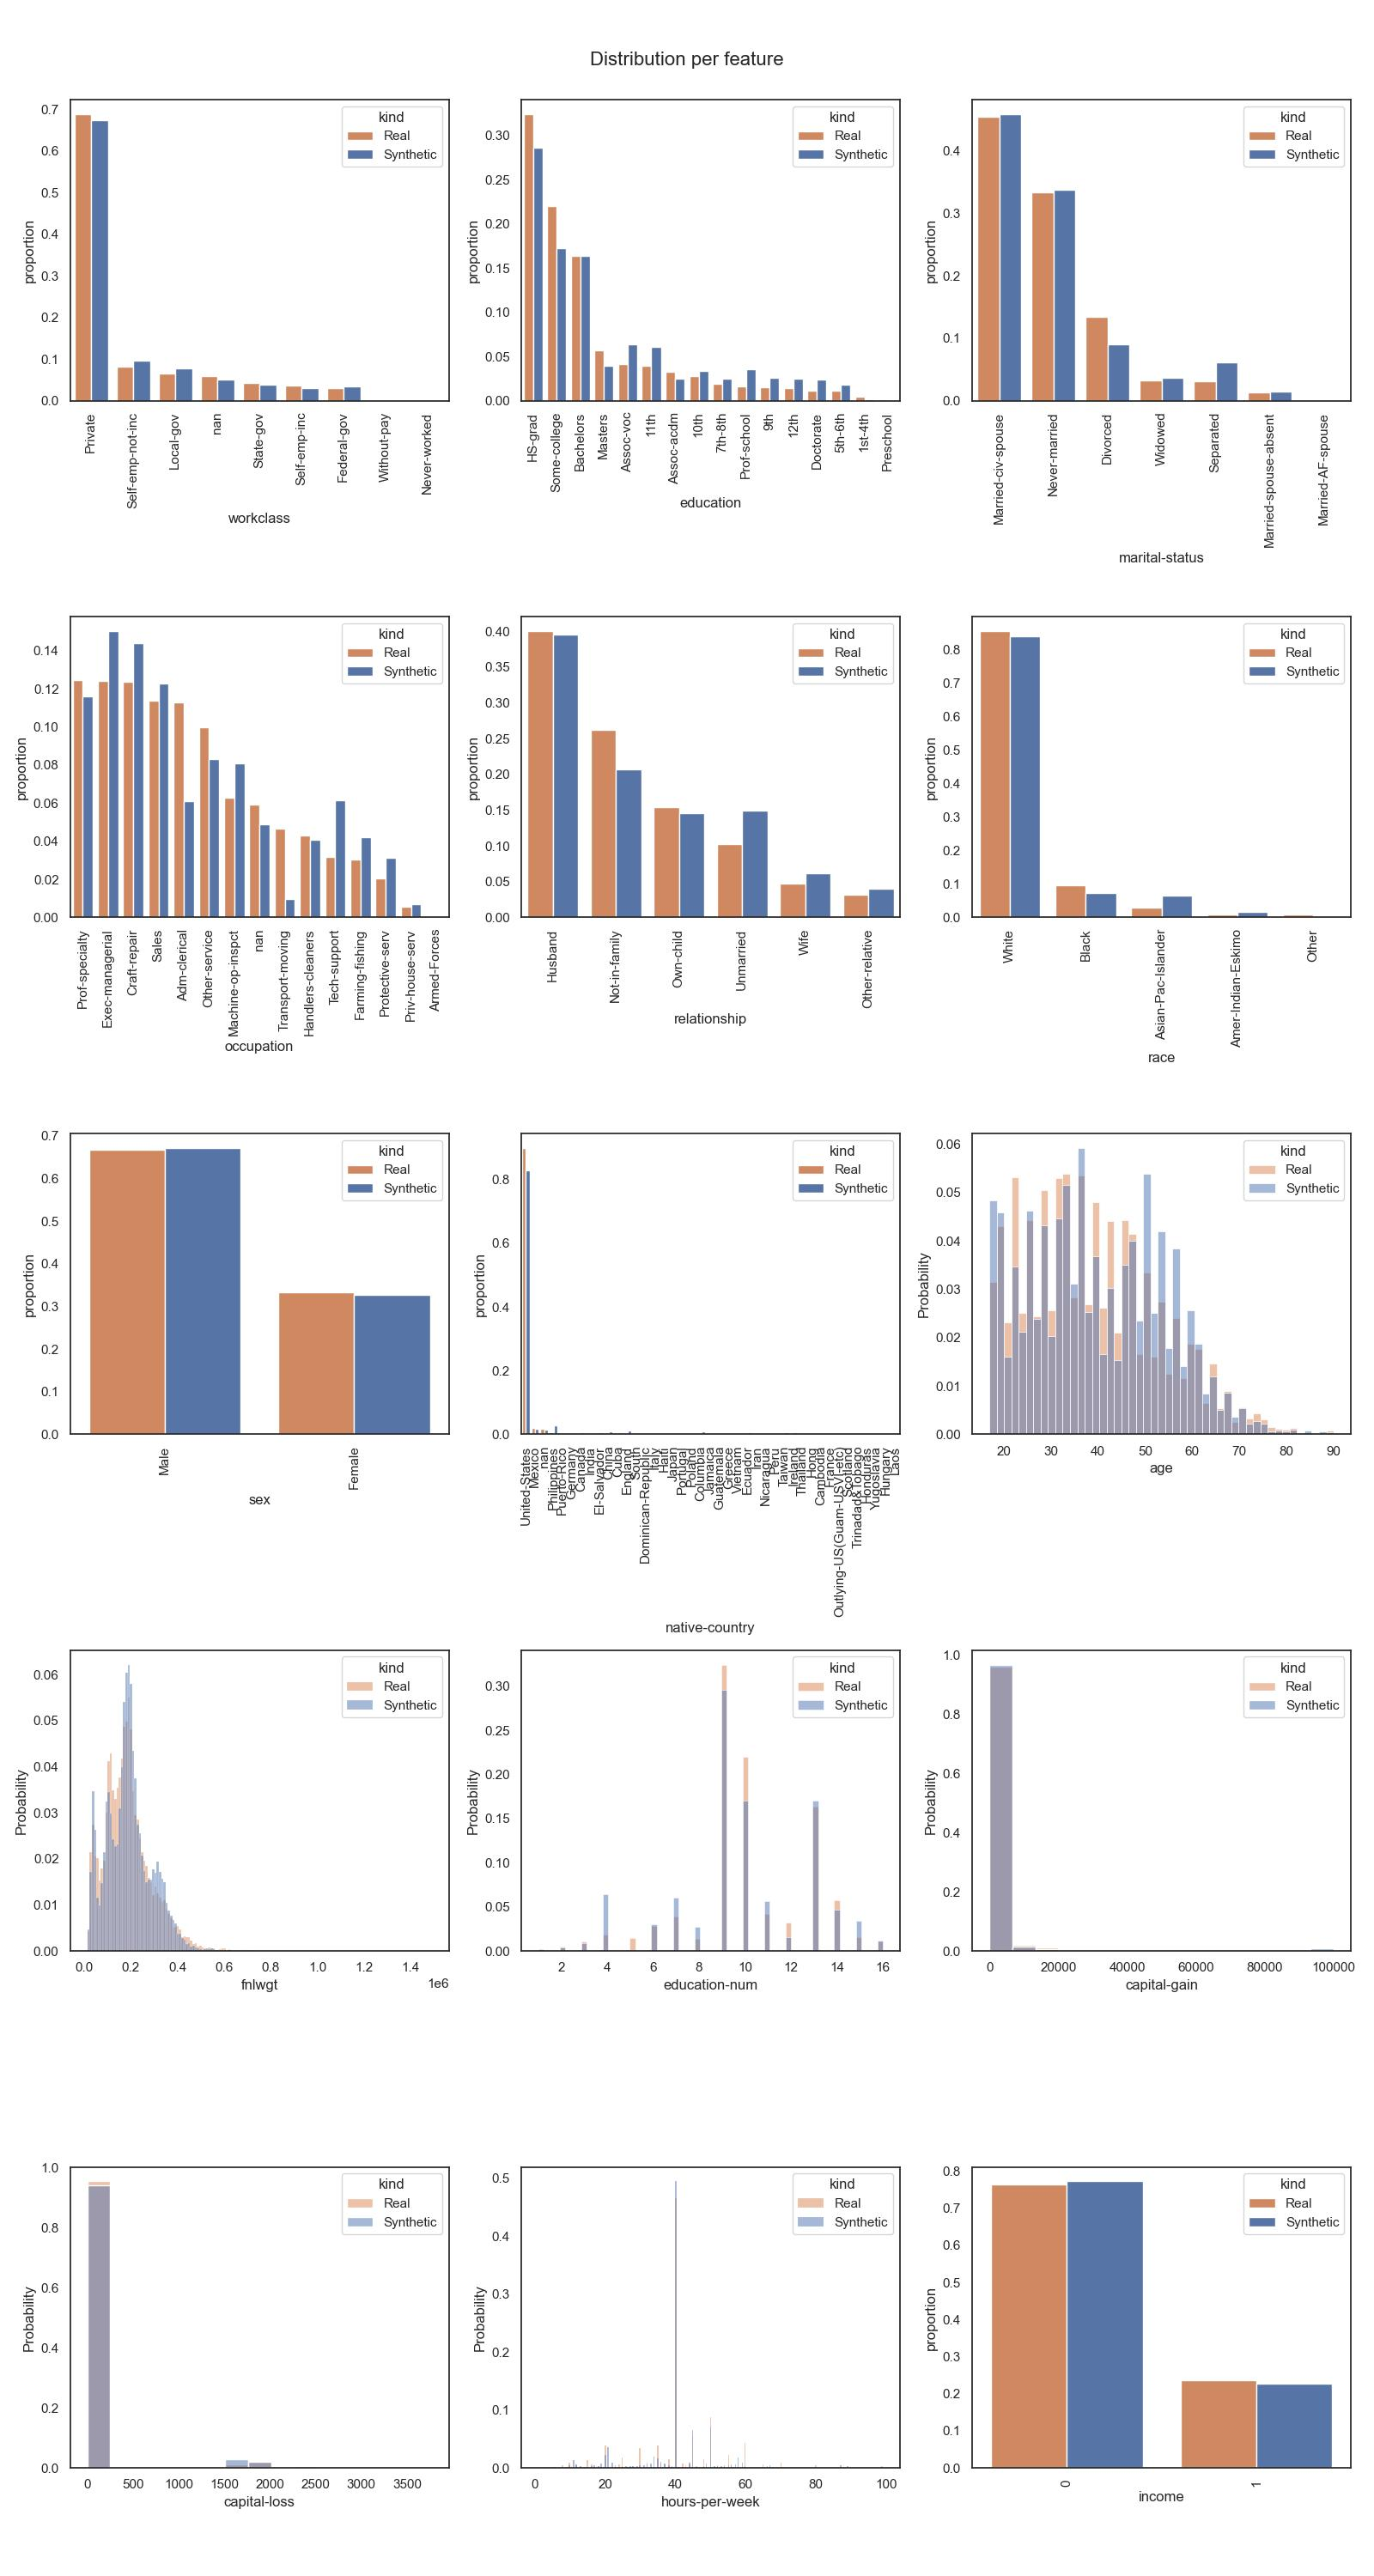
\includegraphics[height=\textheight,width=\linewidth,keepaspectratio]{images/distributions_full/ctabgan_simTune.jpg}
			\caption{CTABGAN$^s$}
		\end{subfigure}	
		\hfill
		\begin{subfigure}{0.3\linewidth}
			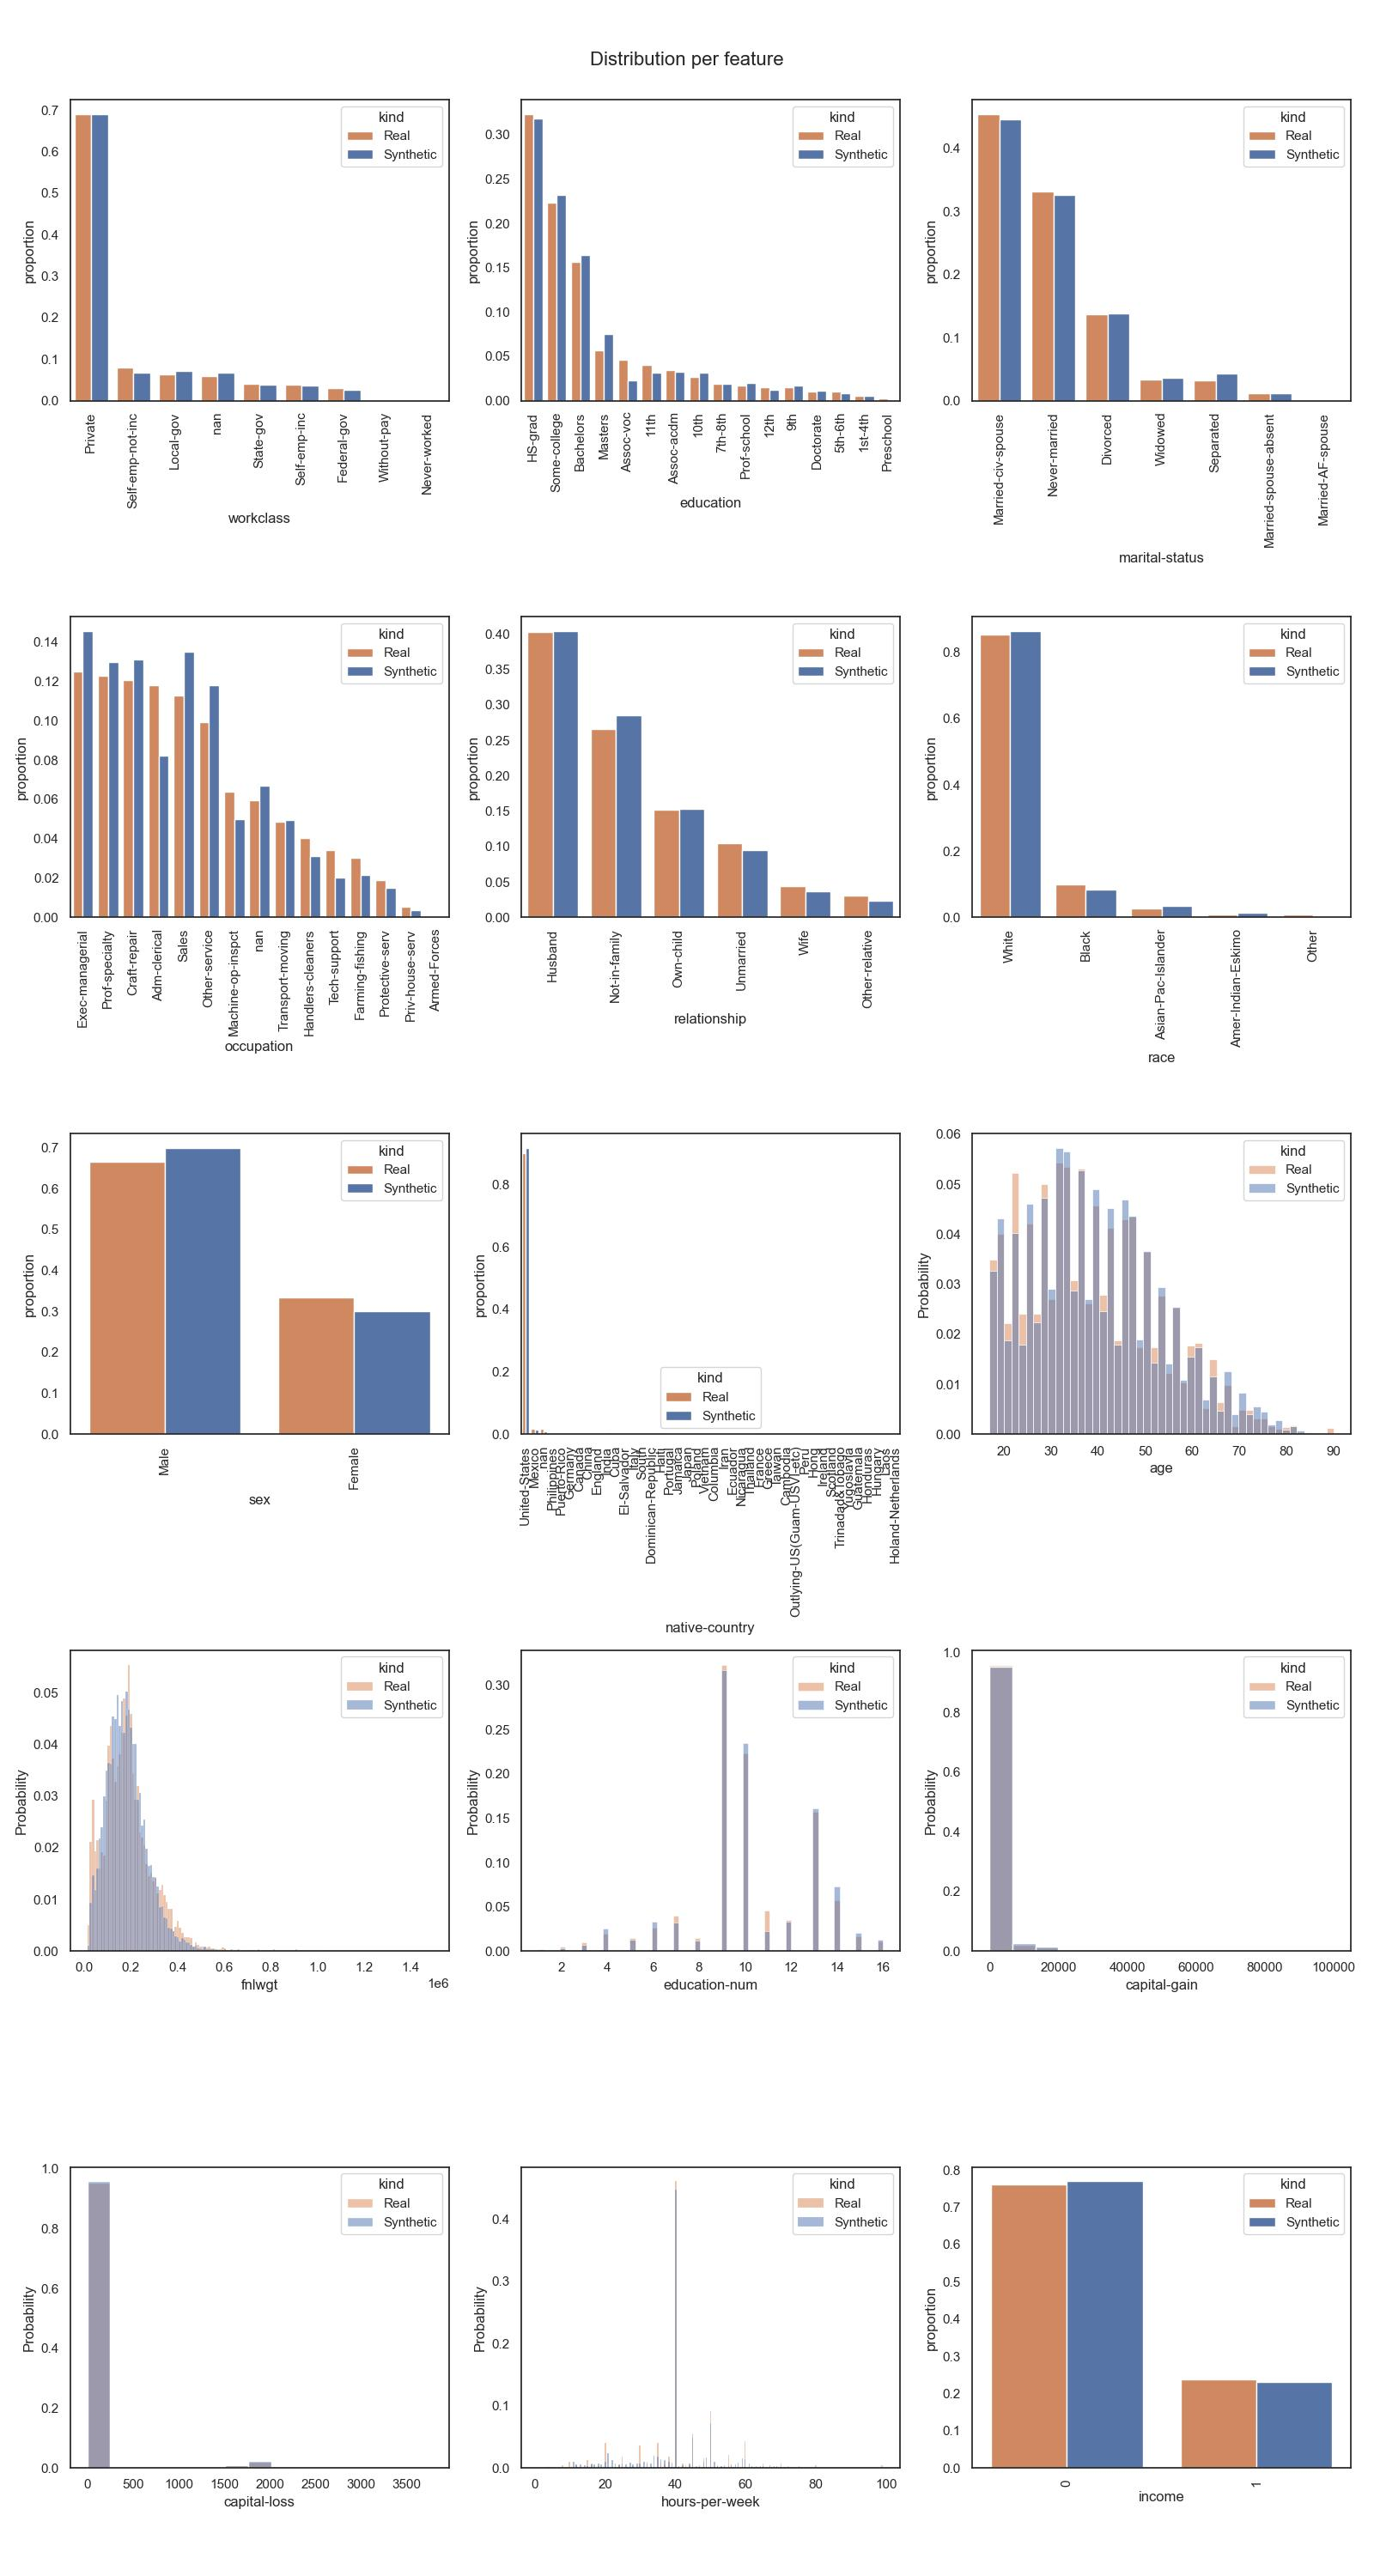
\includegraphics[height=\textheight,width=\linewidth,keepaspectratio]{images/distributions_full/ctabgan+_simTune.jpg}
			\caption{CTABGAN+$^s$}
		\end{subfigure}	
		\hfill
		\caption[Distribution plots CTABGAN Models]{Distribution plots for CTABGAN$^{ml}$, CTABGAN$^s$ and CTABGAN+$^s$}
		\label{fig_a:dist_1}
	\end{figure}
\end{landscape}
%----------
\newpage
\begin{landscape}
	\begin{figure}[h]
		\centering
		\hfill
		\begin{subfigure}{0.3\linewidth}
			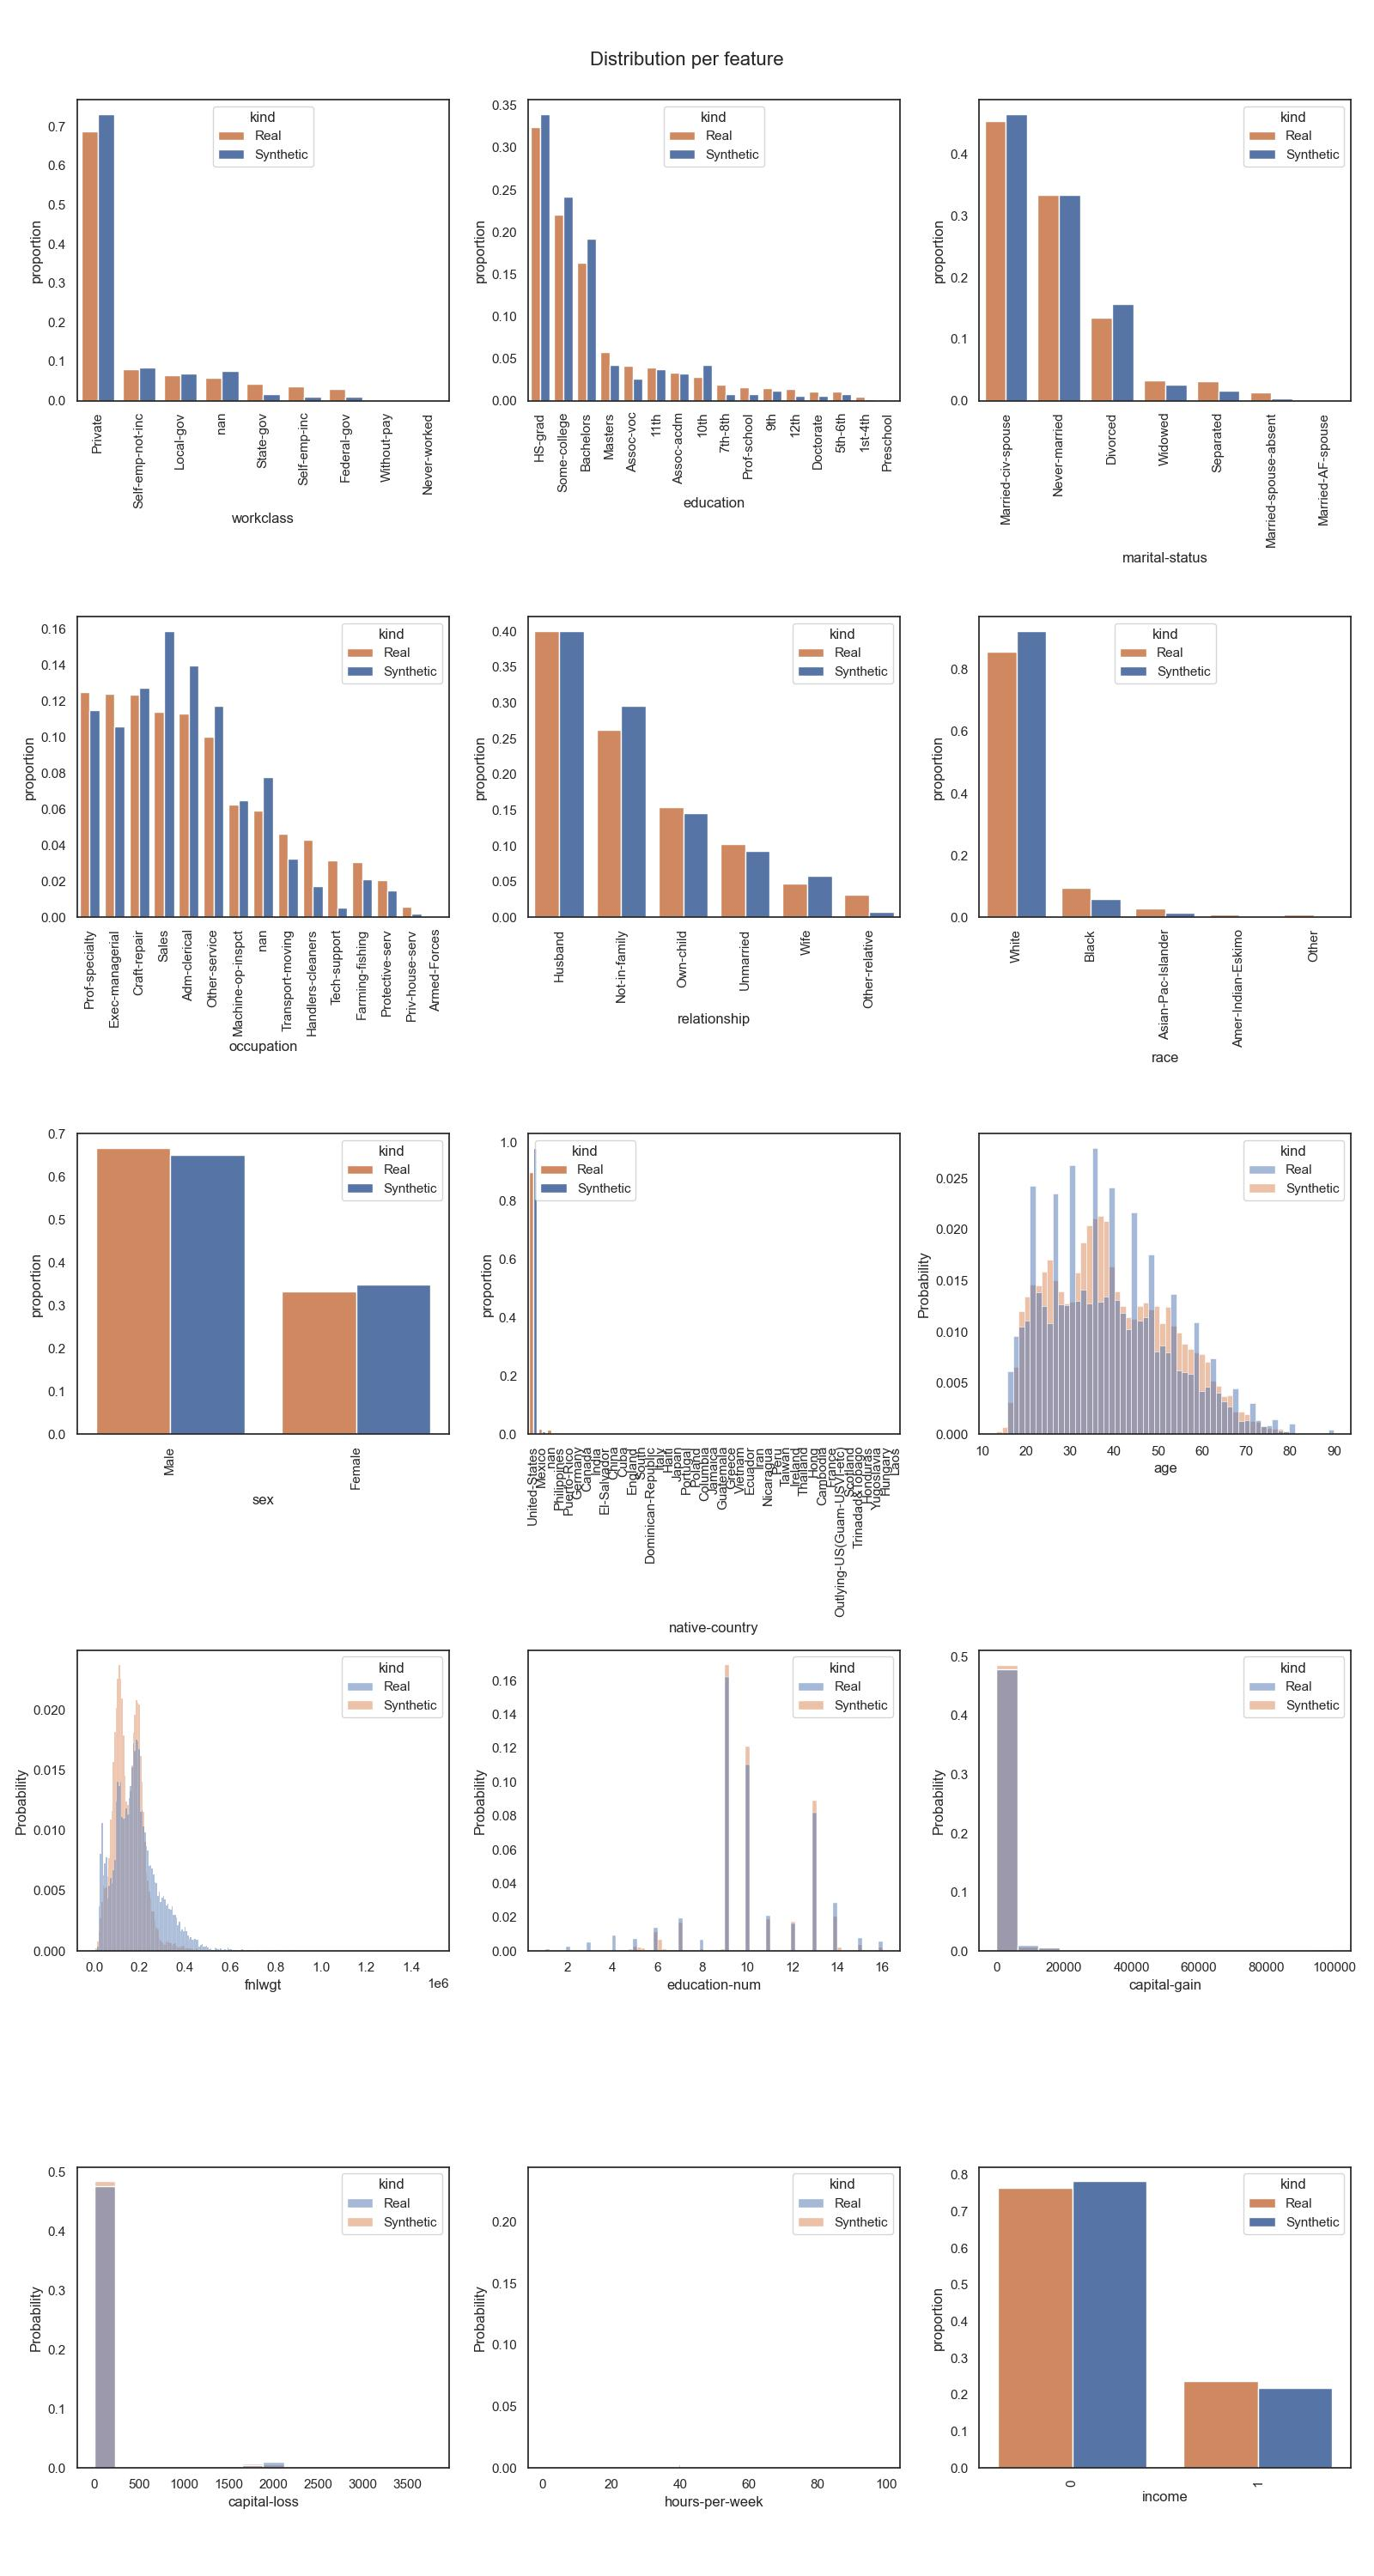
\includegraphics[height=\textheight,width=\linewidth,keepaspectratio]{images/distributions_full/tvae.jpg}
			\caption{TVAE$^{ml}$}
		\end{subfigure}		
		\hfill
		\begin{subfigure}{0.3\linewidth}
			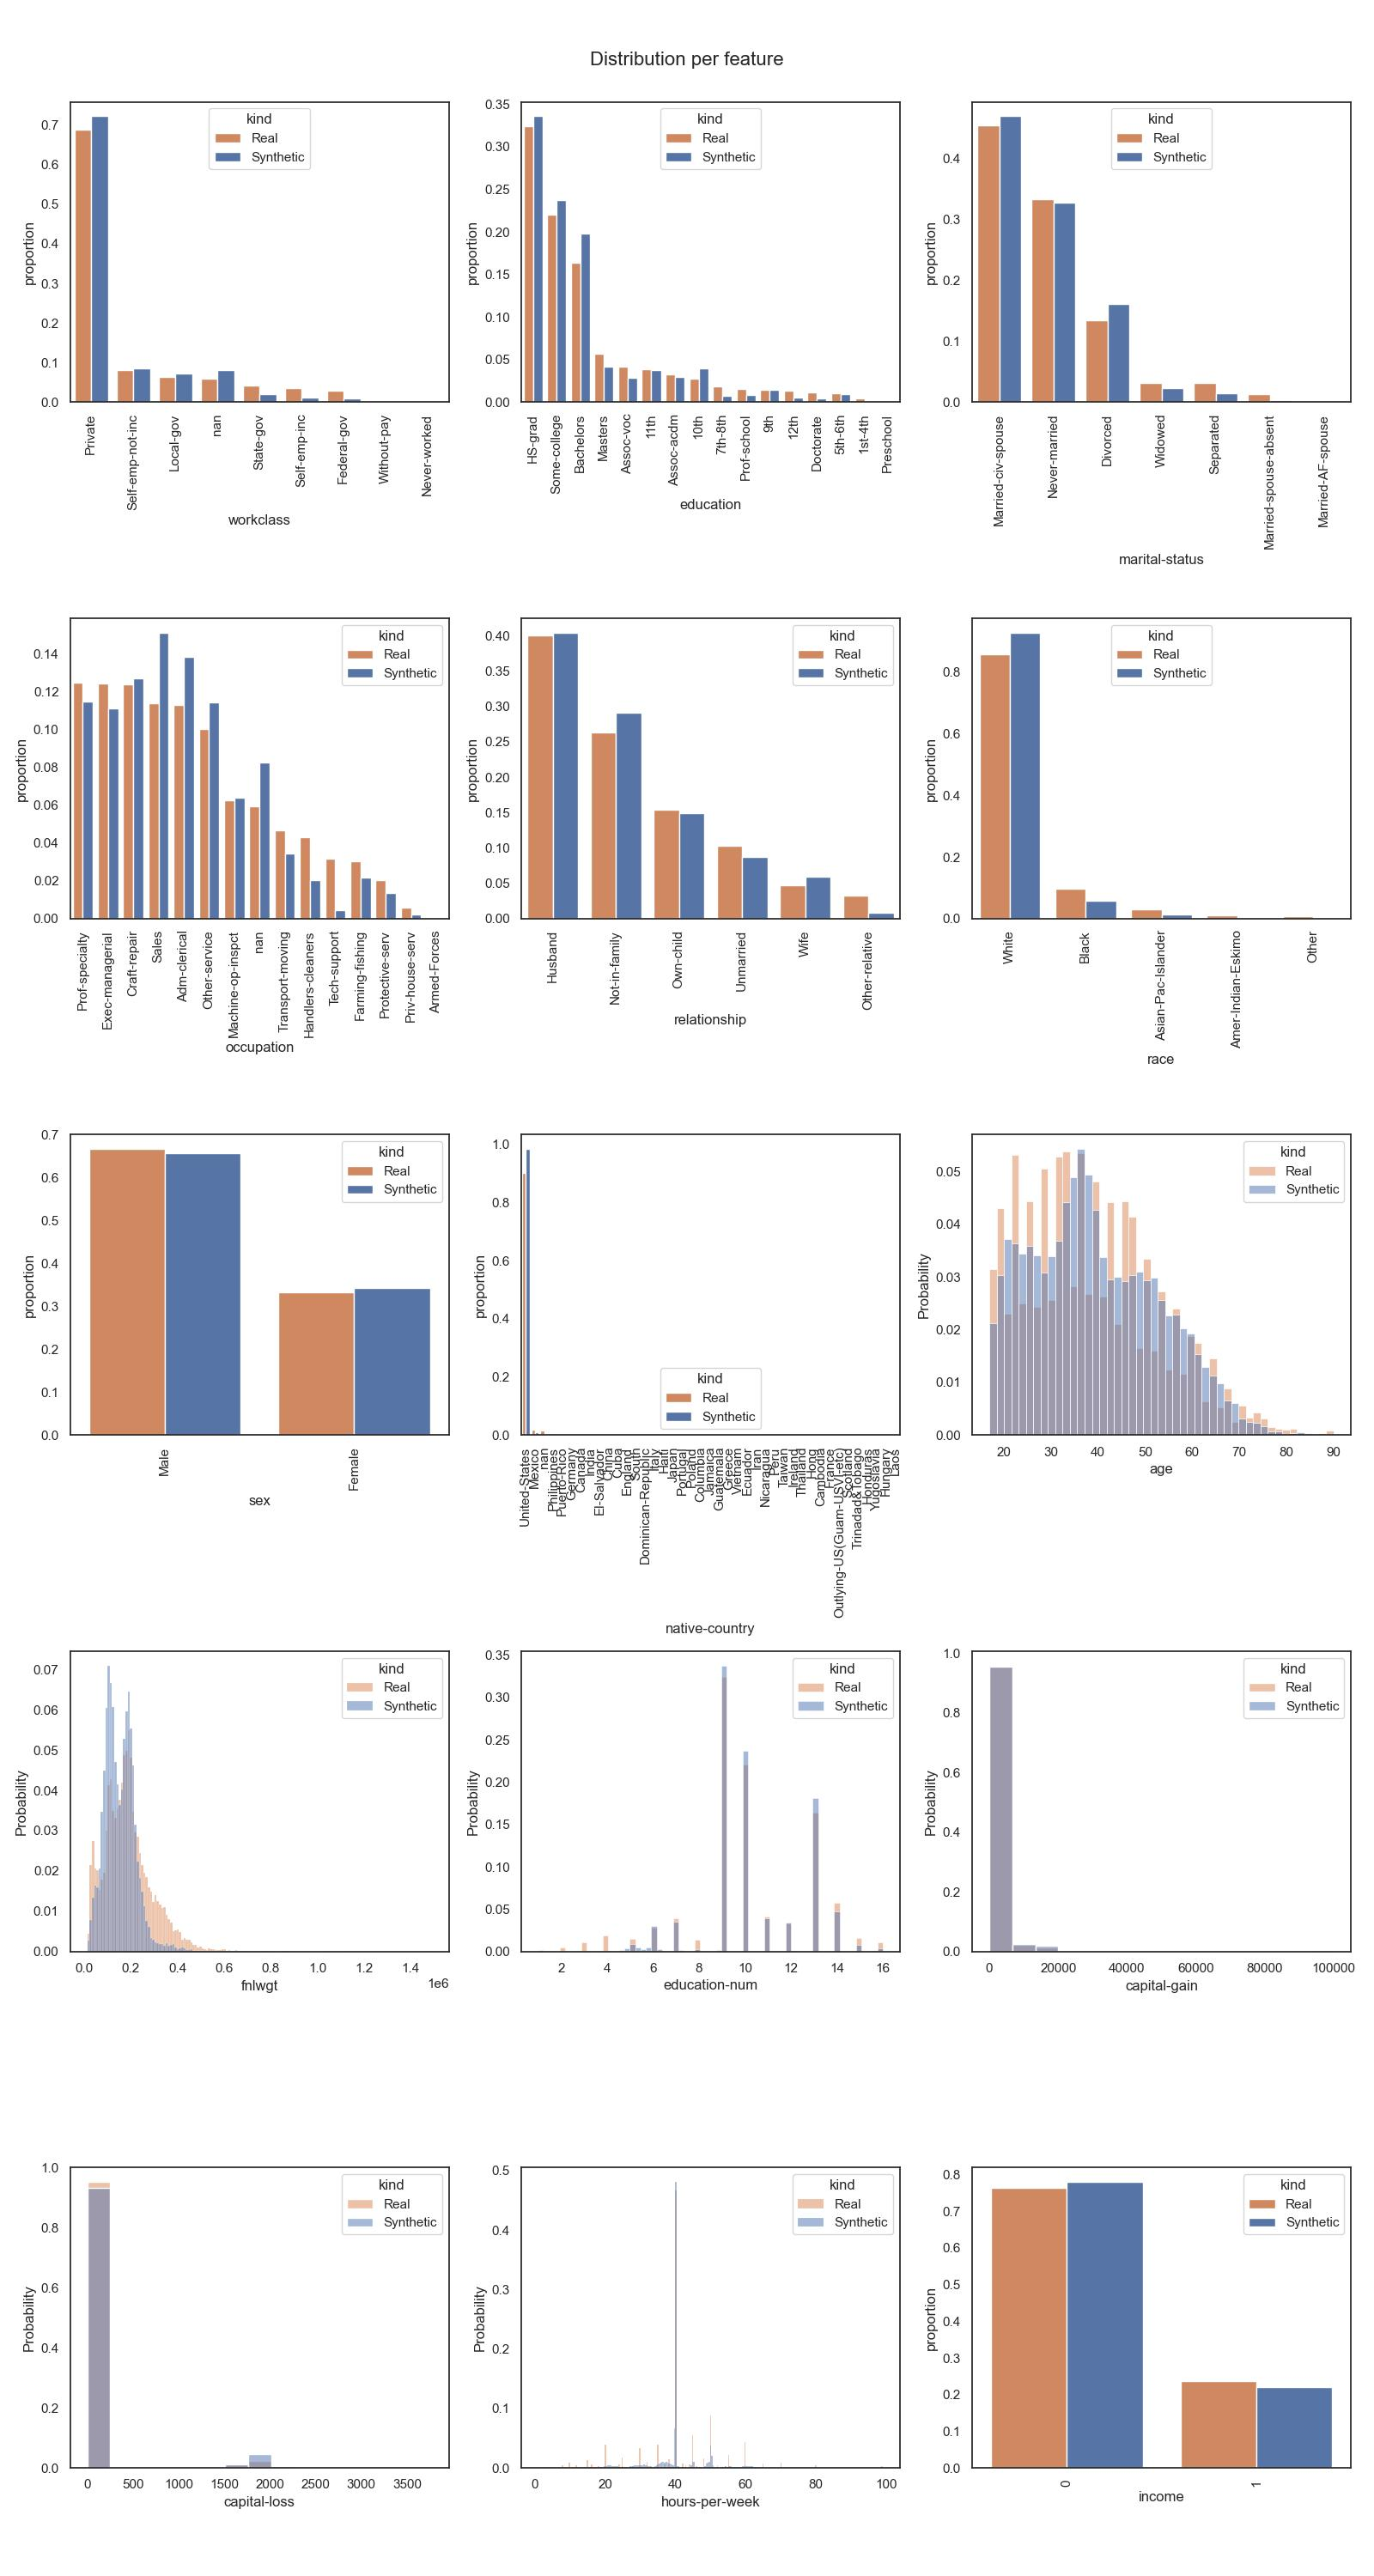
\includegraphics[height=\textheight,width=\linewidth,keepaspectratio]{images/distributions_full/tvae_simTune.jpg}
			\caption{TVAE$^s$}
		\end{subfigure}
		\hfill
		\begin{subfigure}{0.3\linewidth}
			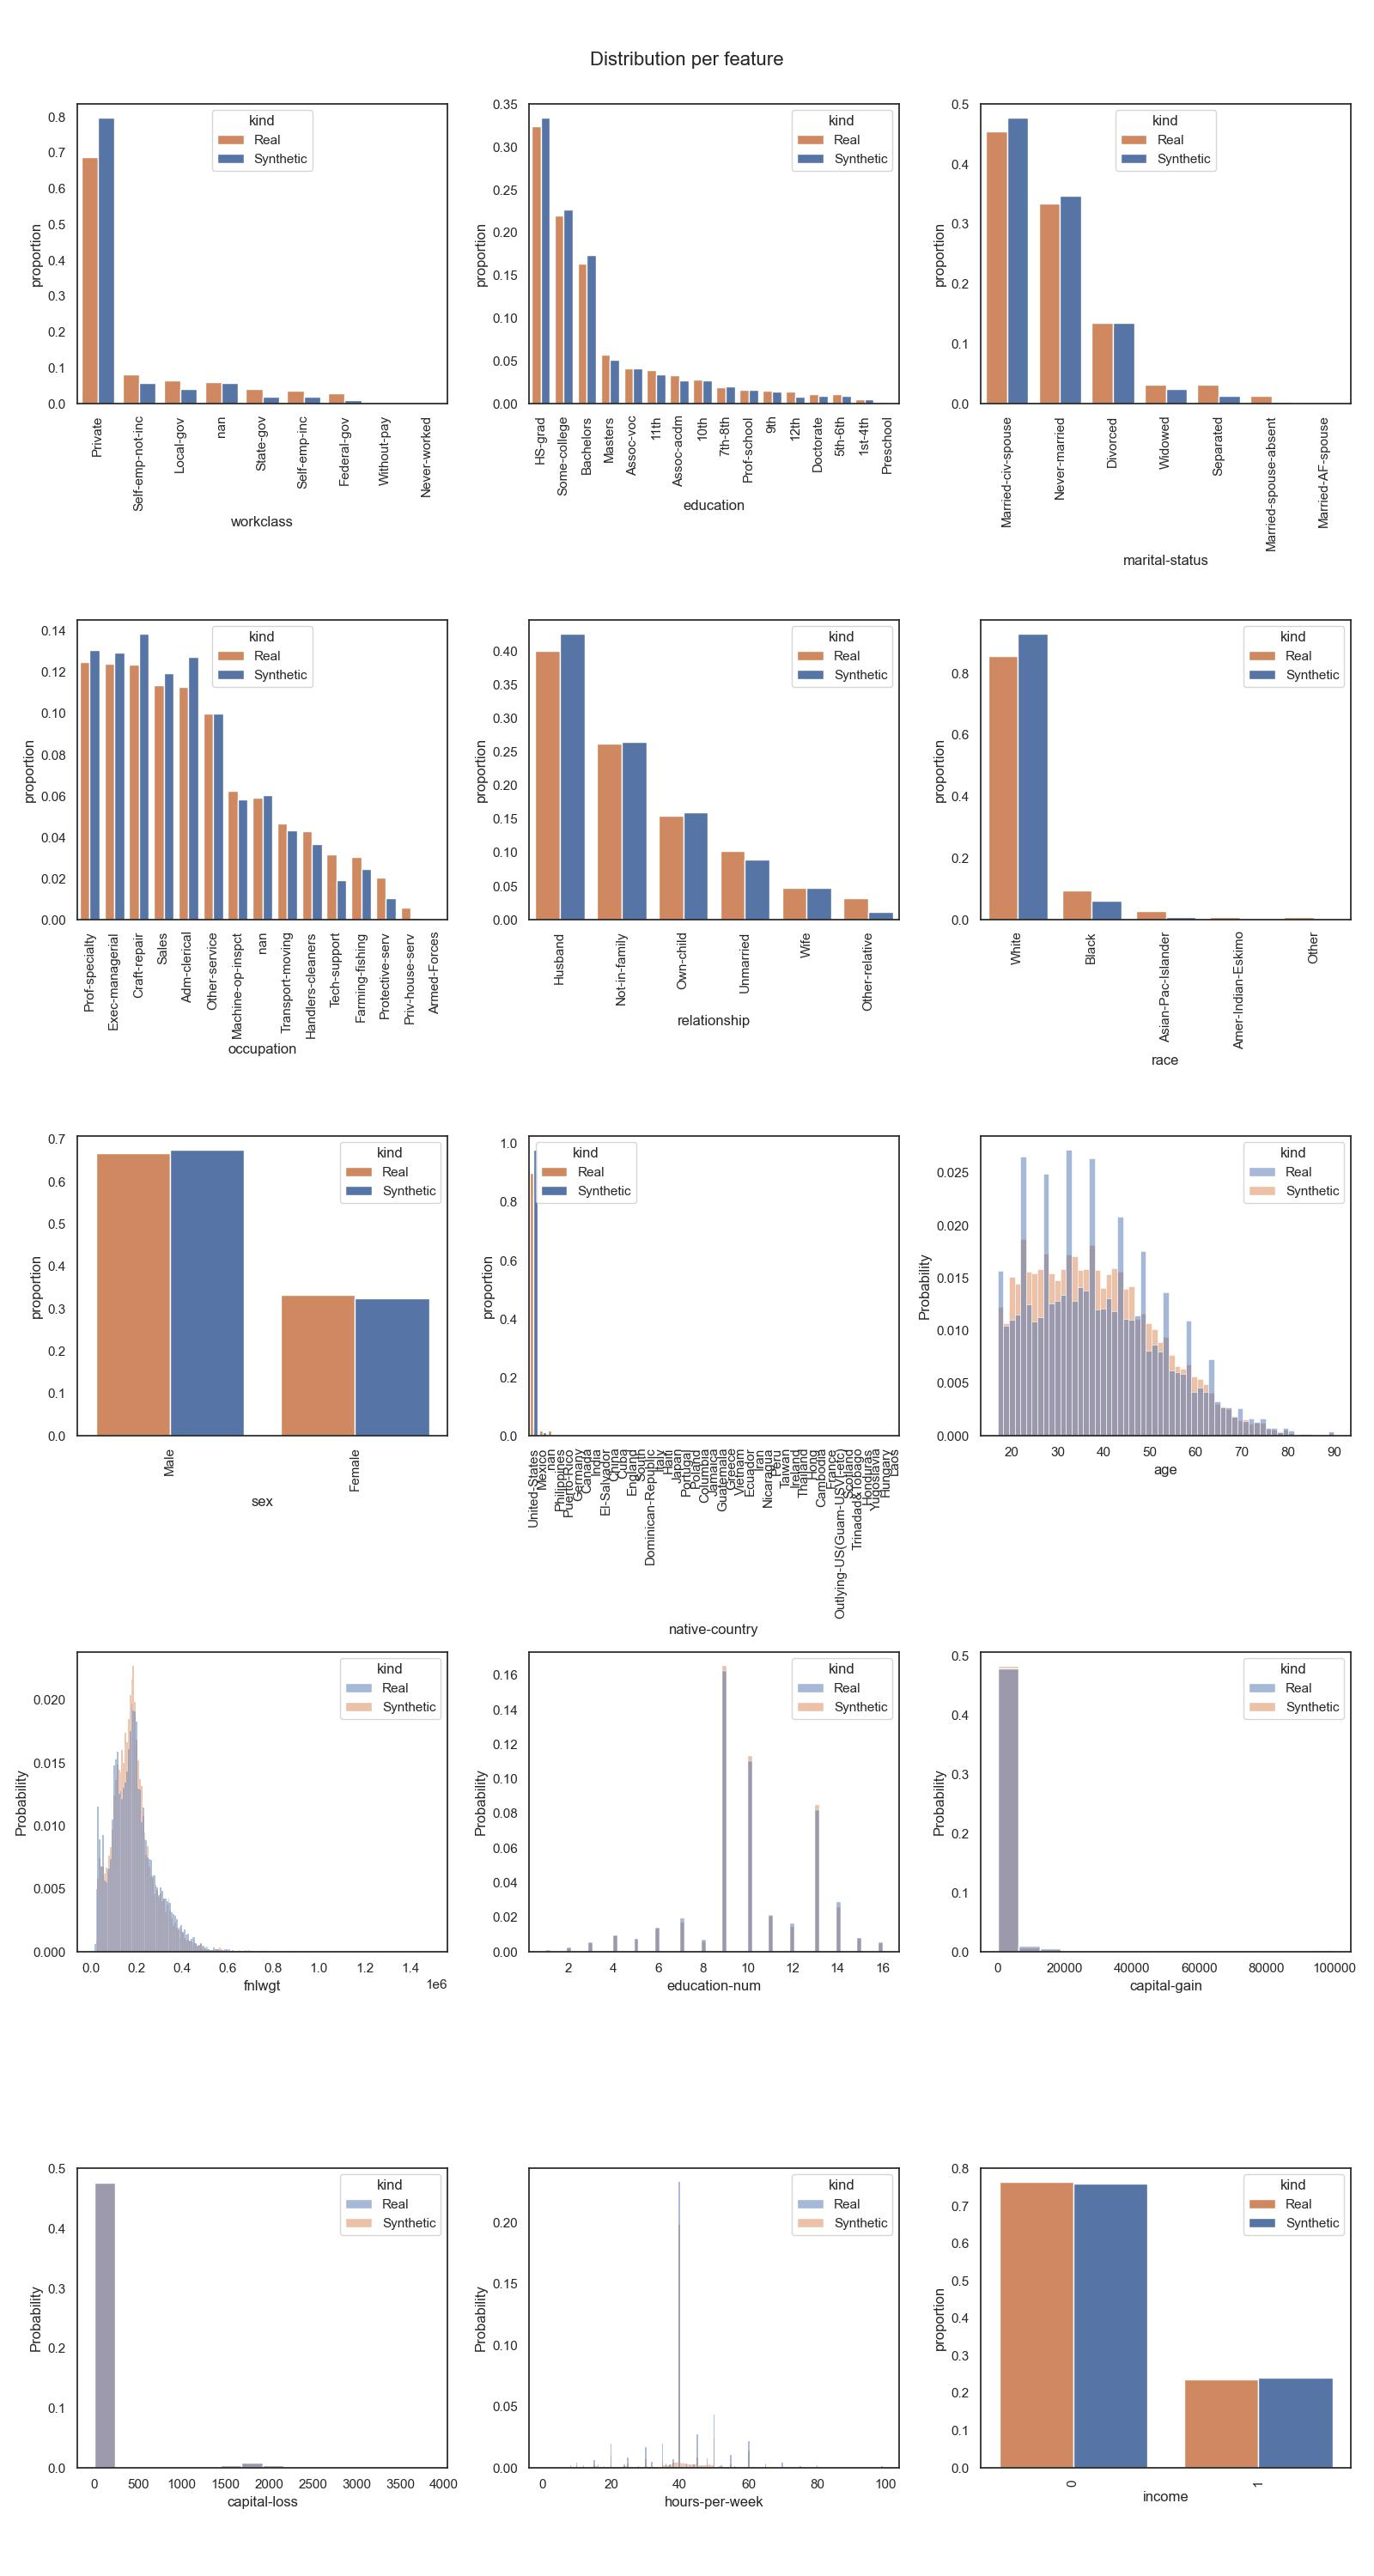
\includegraphics[height=\textheight,width=\linewidth,keepaspectratio]{images/distributions_full/smote.jpg}
			\caption{SMOTE}
		\end{subfigure}
		\caption[Distribution plots Baseline Models]{Distribution plots for TVAE$^{ml}$, TVAE$^s$ and SMOTE}
		\label{fig_a:dist_2}
	\end{figure}
\end{landscape}
%----------
\newpage
\begin{landscape}
	\begin{figure}[h]
		\centering
		\hfill
		\begin{subfigure}{0.3\linewidth}
			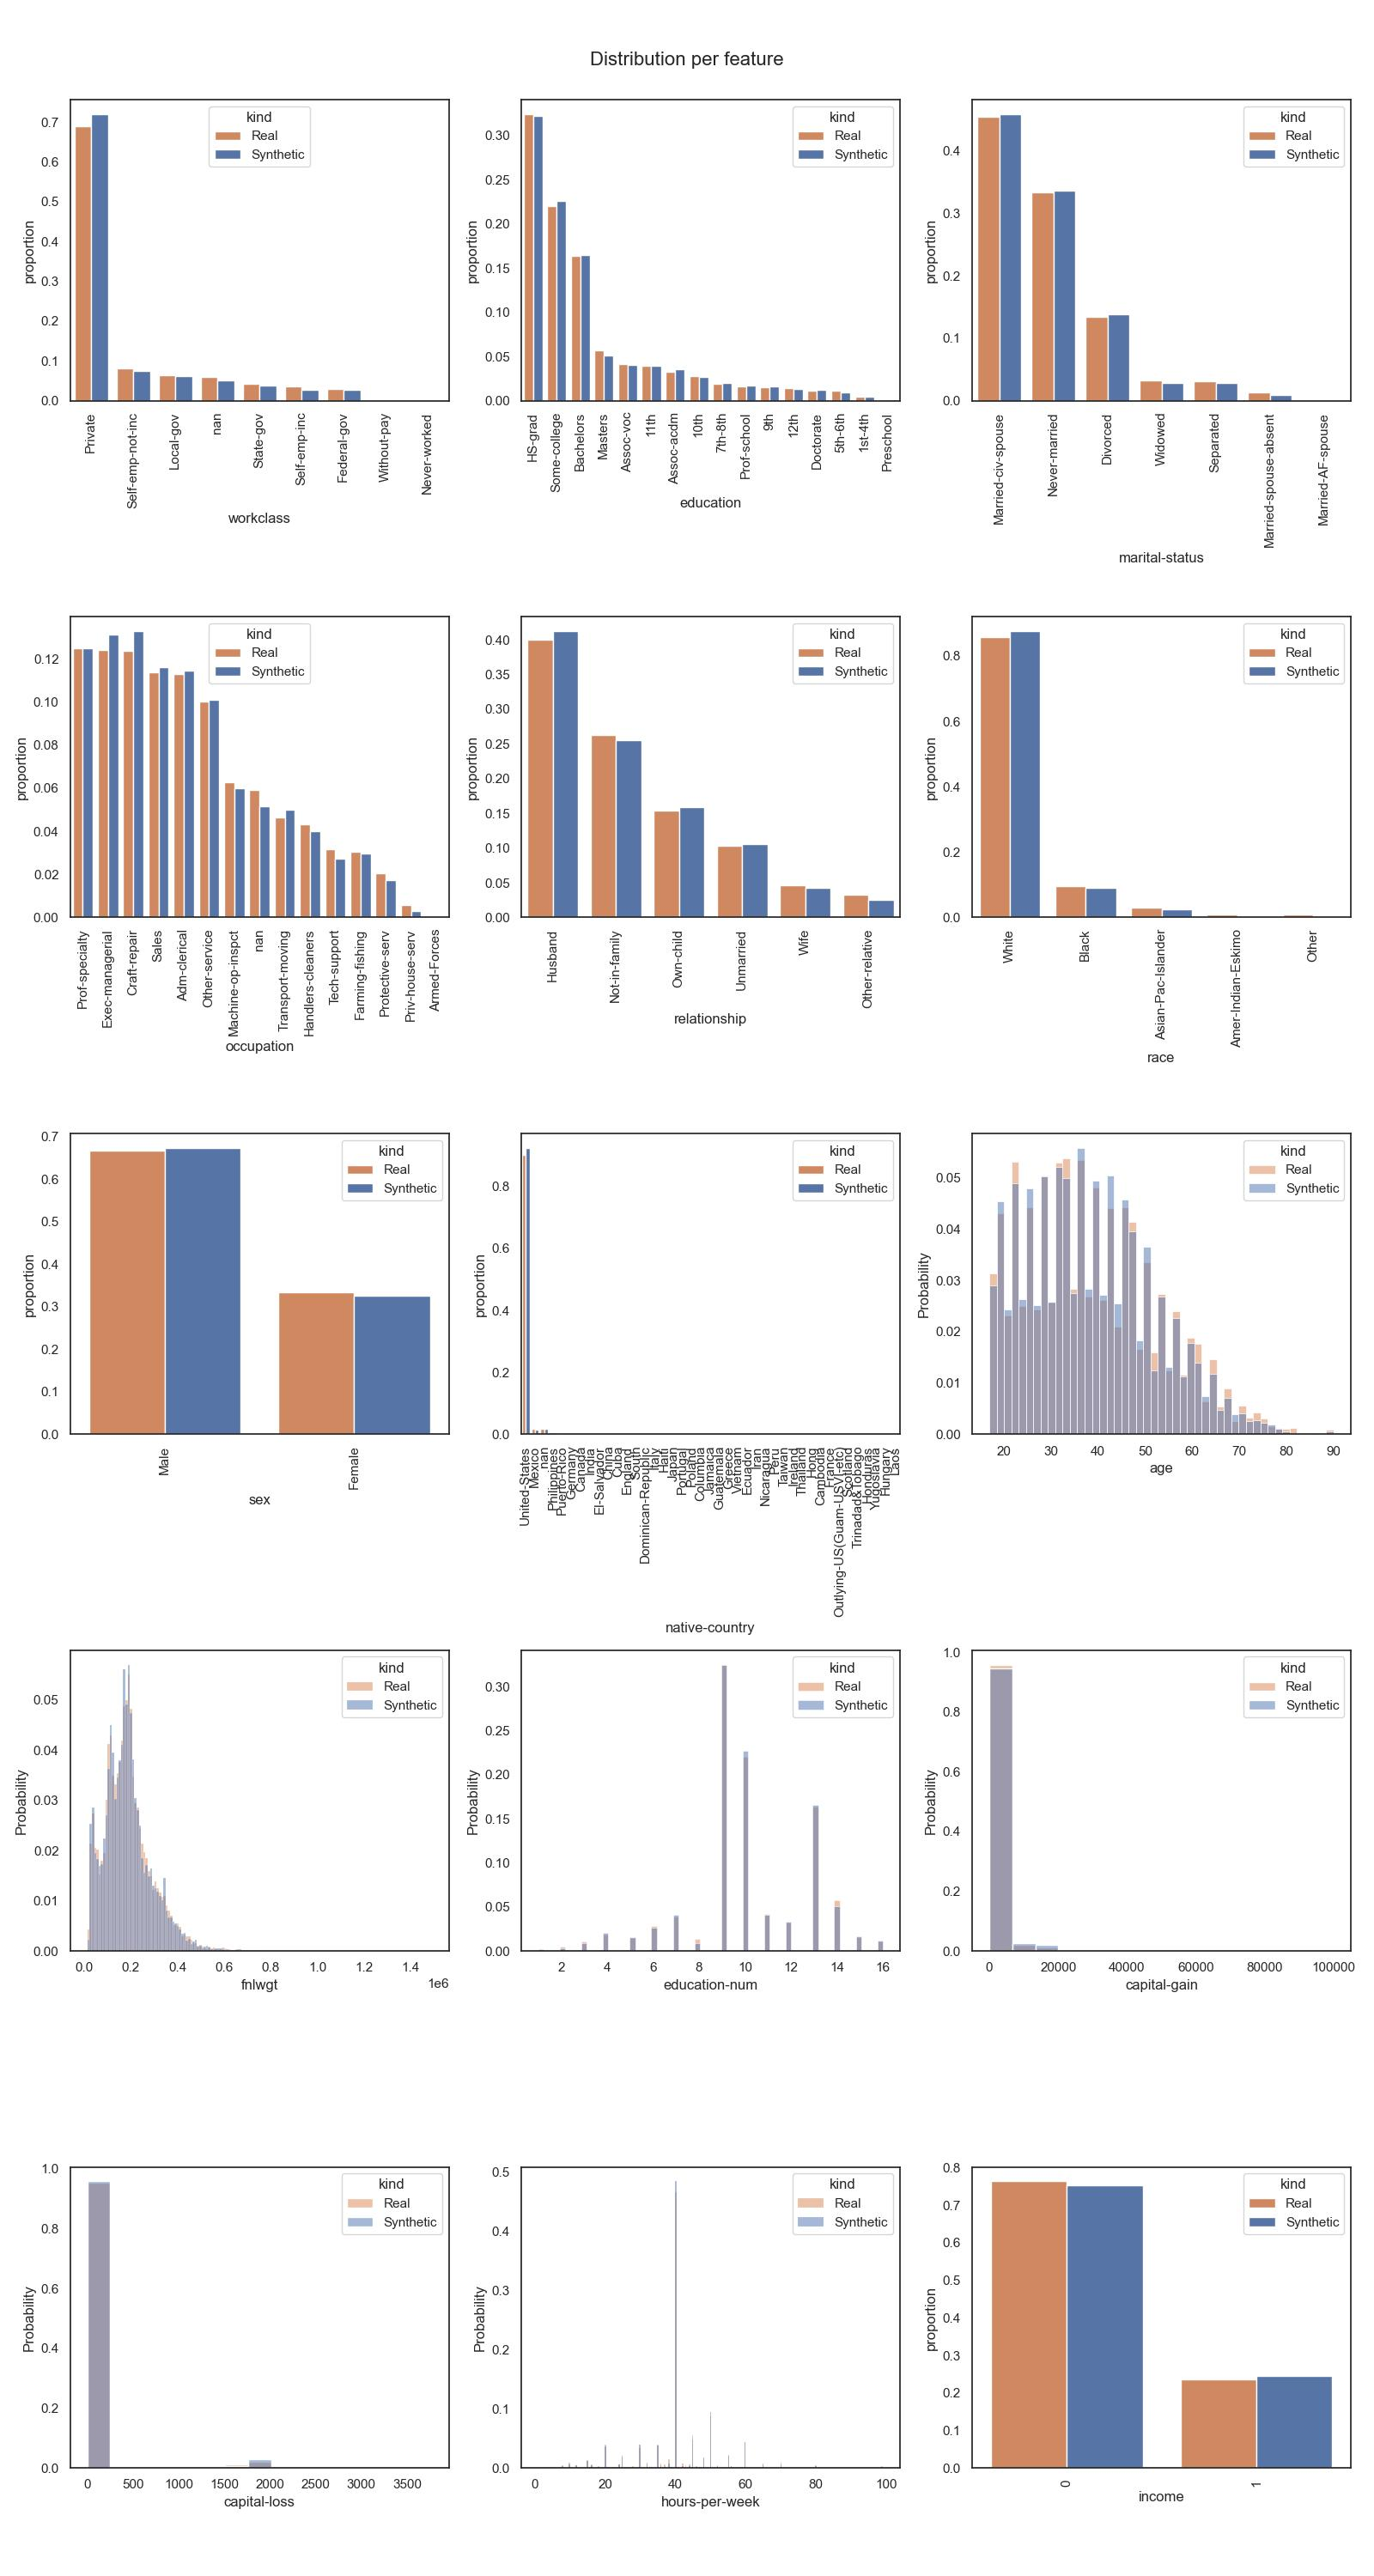
\includegraphics[height=\textheight,width=\linewidth,keepaspectratio]{images/distributions_full/tab-ddpm.jpg}
			\caption{TabDDPM$^{ml}_q$}
		\end{subfigure}
		\hfill
		\begin{subfigure}{0.3\linewidth}
			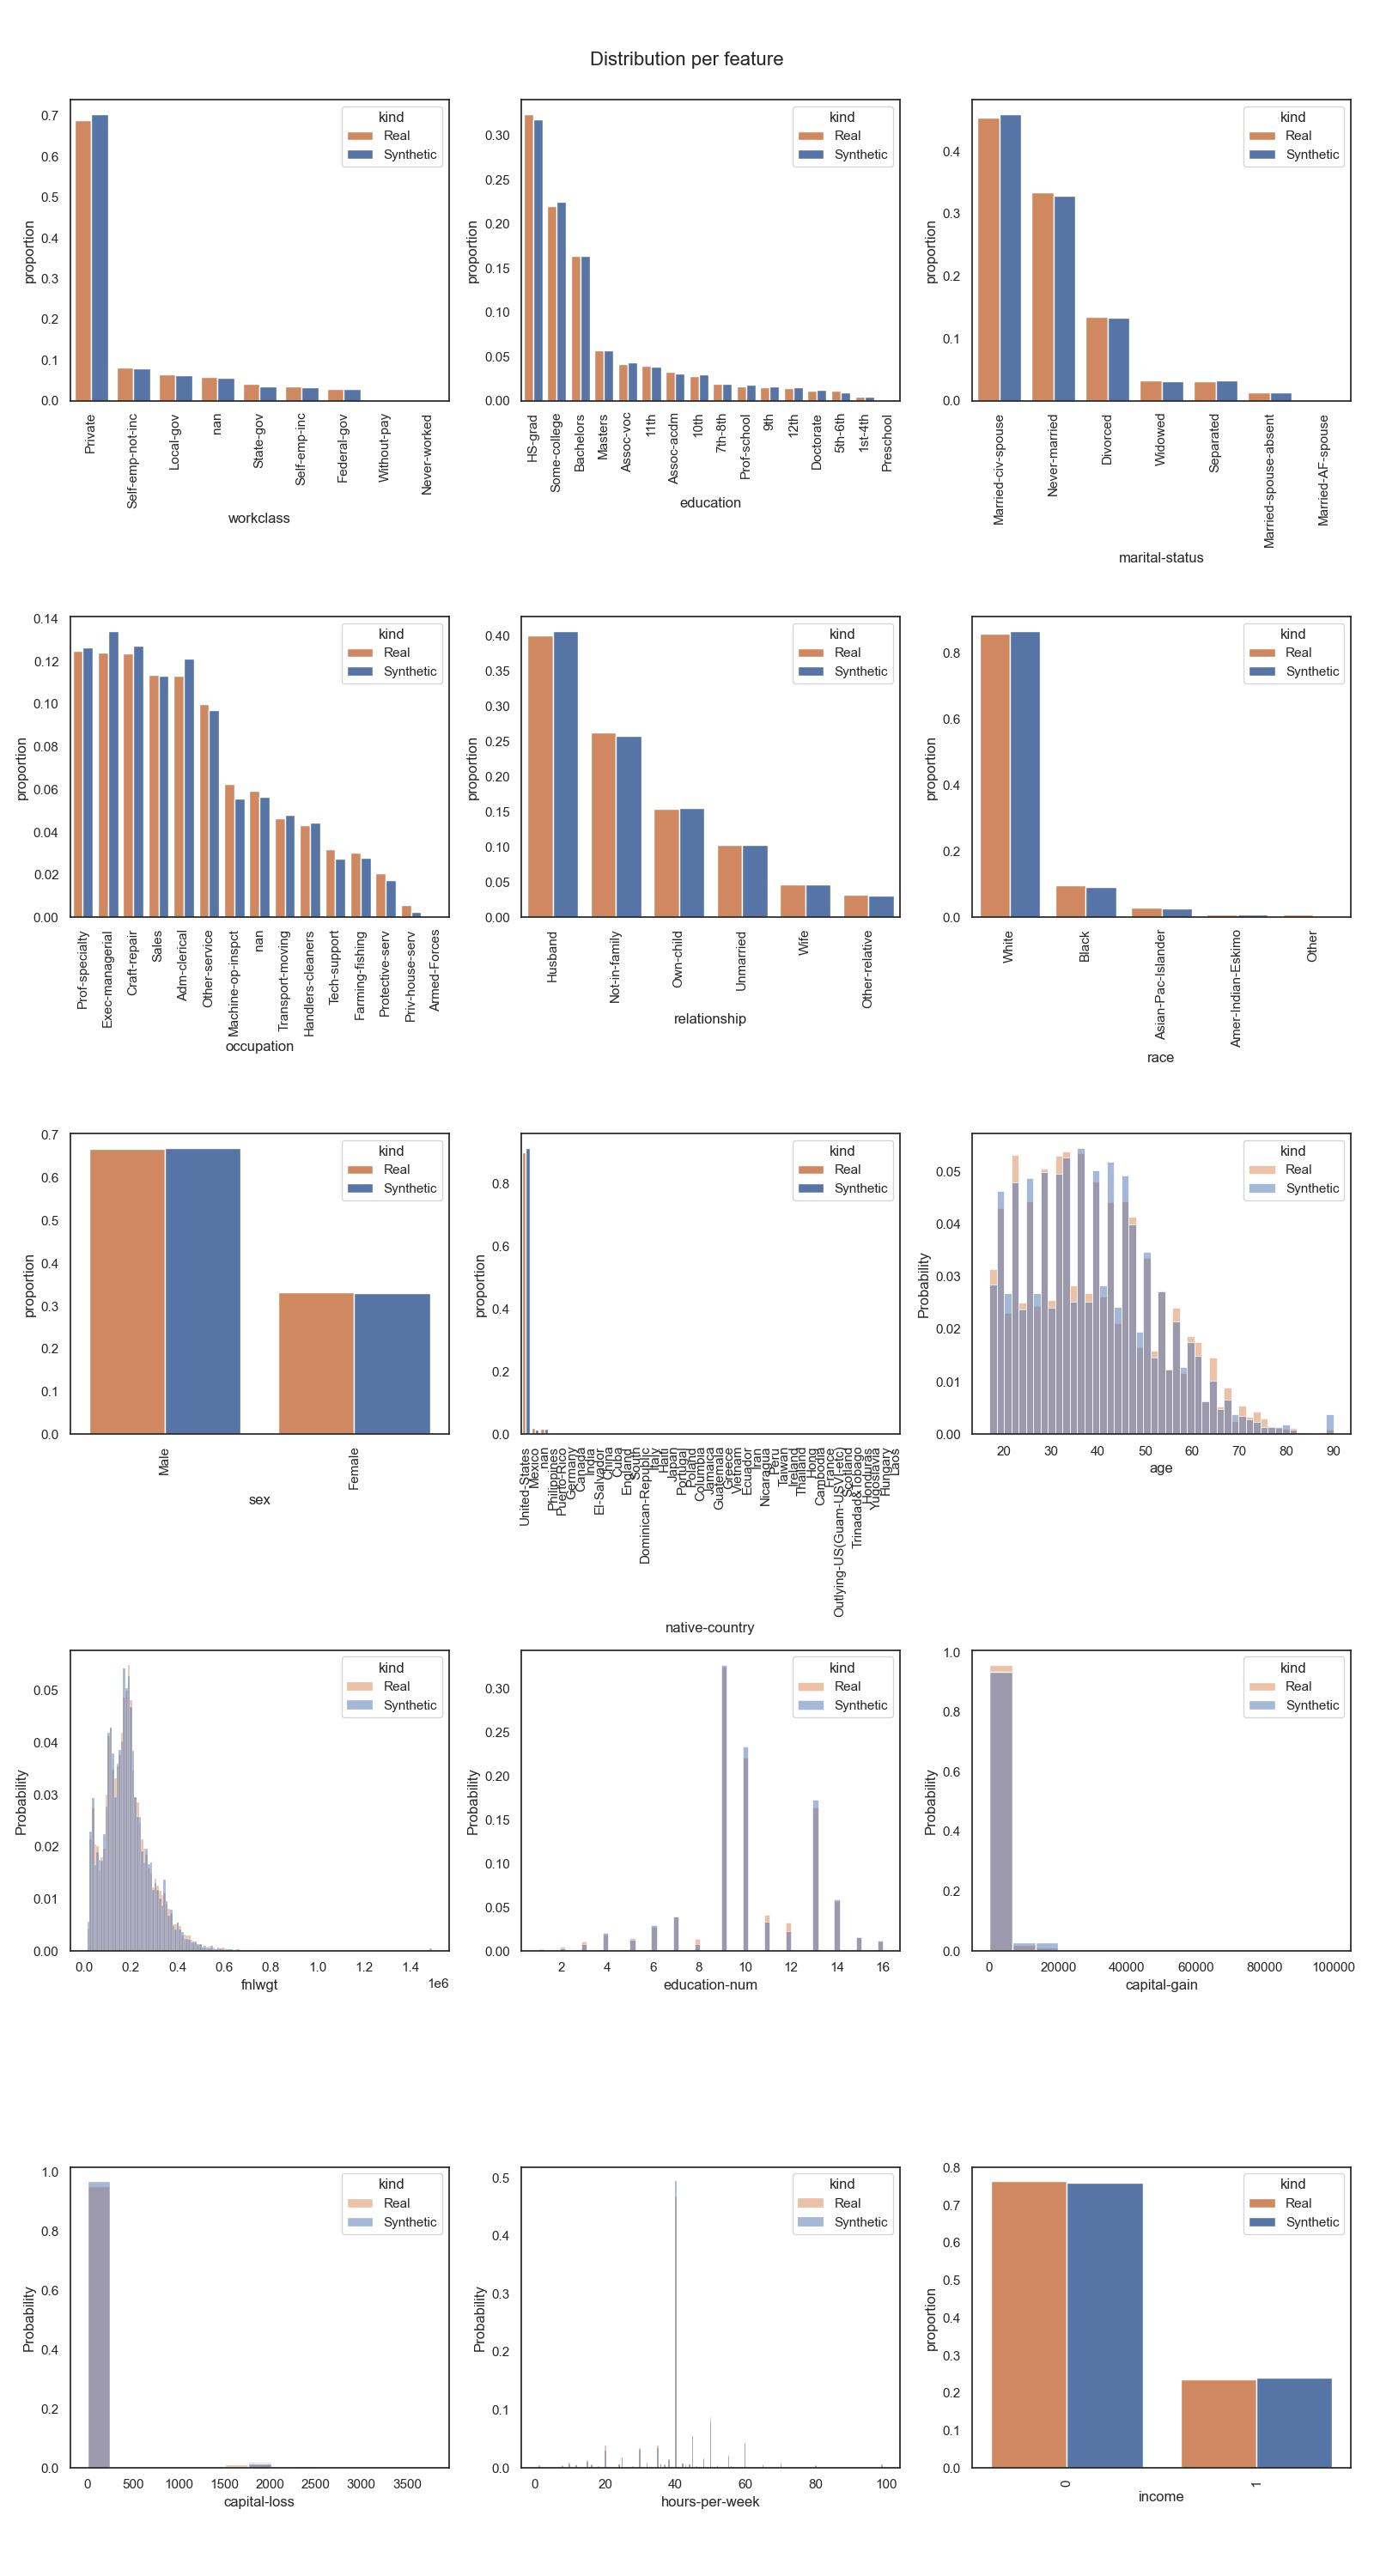
\includegraphics[height=\textheight,width=\linewidth,keepaspectratio]{images/distributions_full/tab-ddpm-simTune.jpg}
			\caption{TabDDPM$^{s}_q$}
		\end{subfigure}
		\hfill
		\begin{subfigure}{0.3\linewidth}
			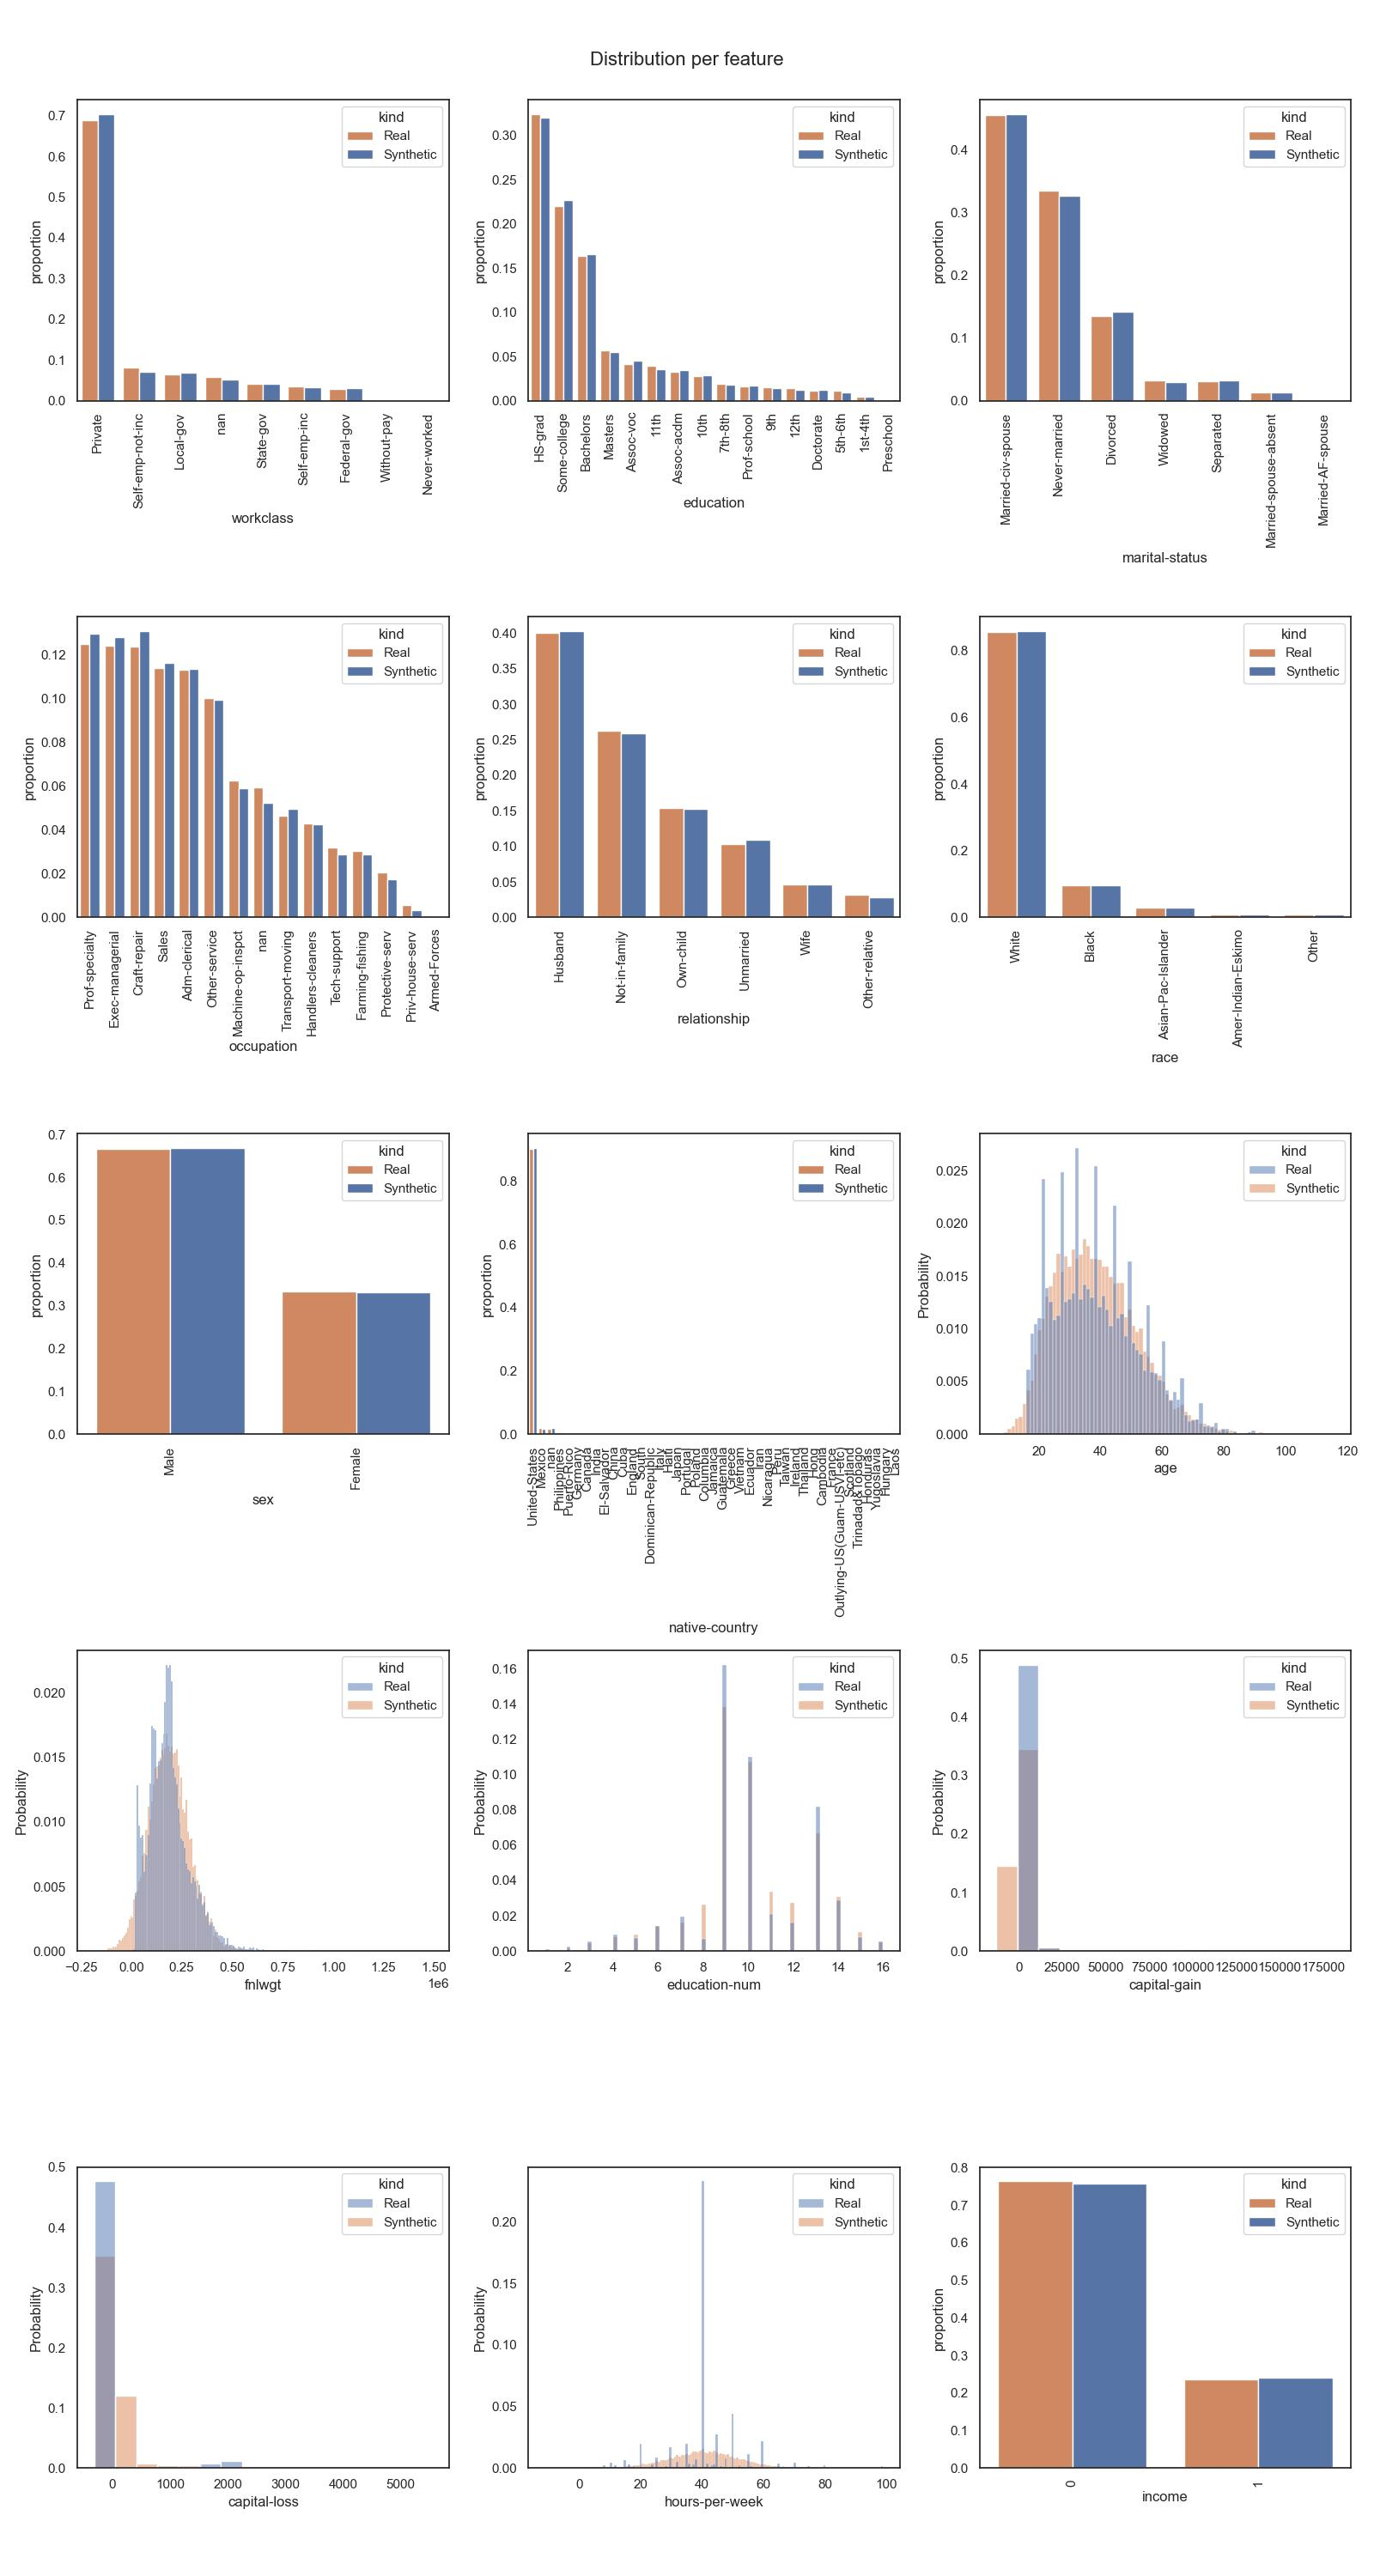
\includegraphics[height=\textheight,width=\linewidth,keepaspectratio]{images/distributions_full/tab-ddpm-simTune-minmax.jpg}
			\caption{TabDDPM$^{s}_m$}
			\label{fig_a:dist_3_c}
		\end{subfigure}
		\hfill
		\caption[Distribution plots TabDDPM Models]{Distribution plots for TabDDPM variations}
		\label{fig_a:dist_3}
	\end{figure}
\end{landscape}
%----------
\newpage
\begin{landscape}
	\begin{figure}[h]
		\centering
		\hfill
		\begin{subfigure}{0.3\linewidth}
			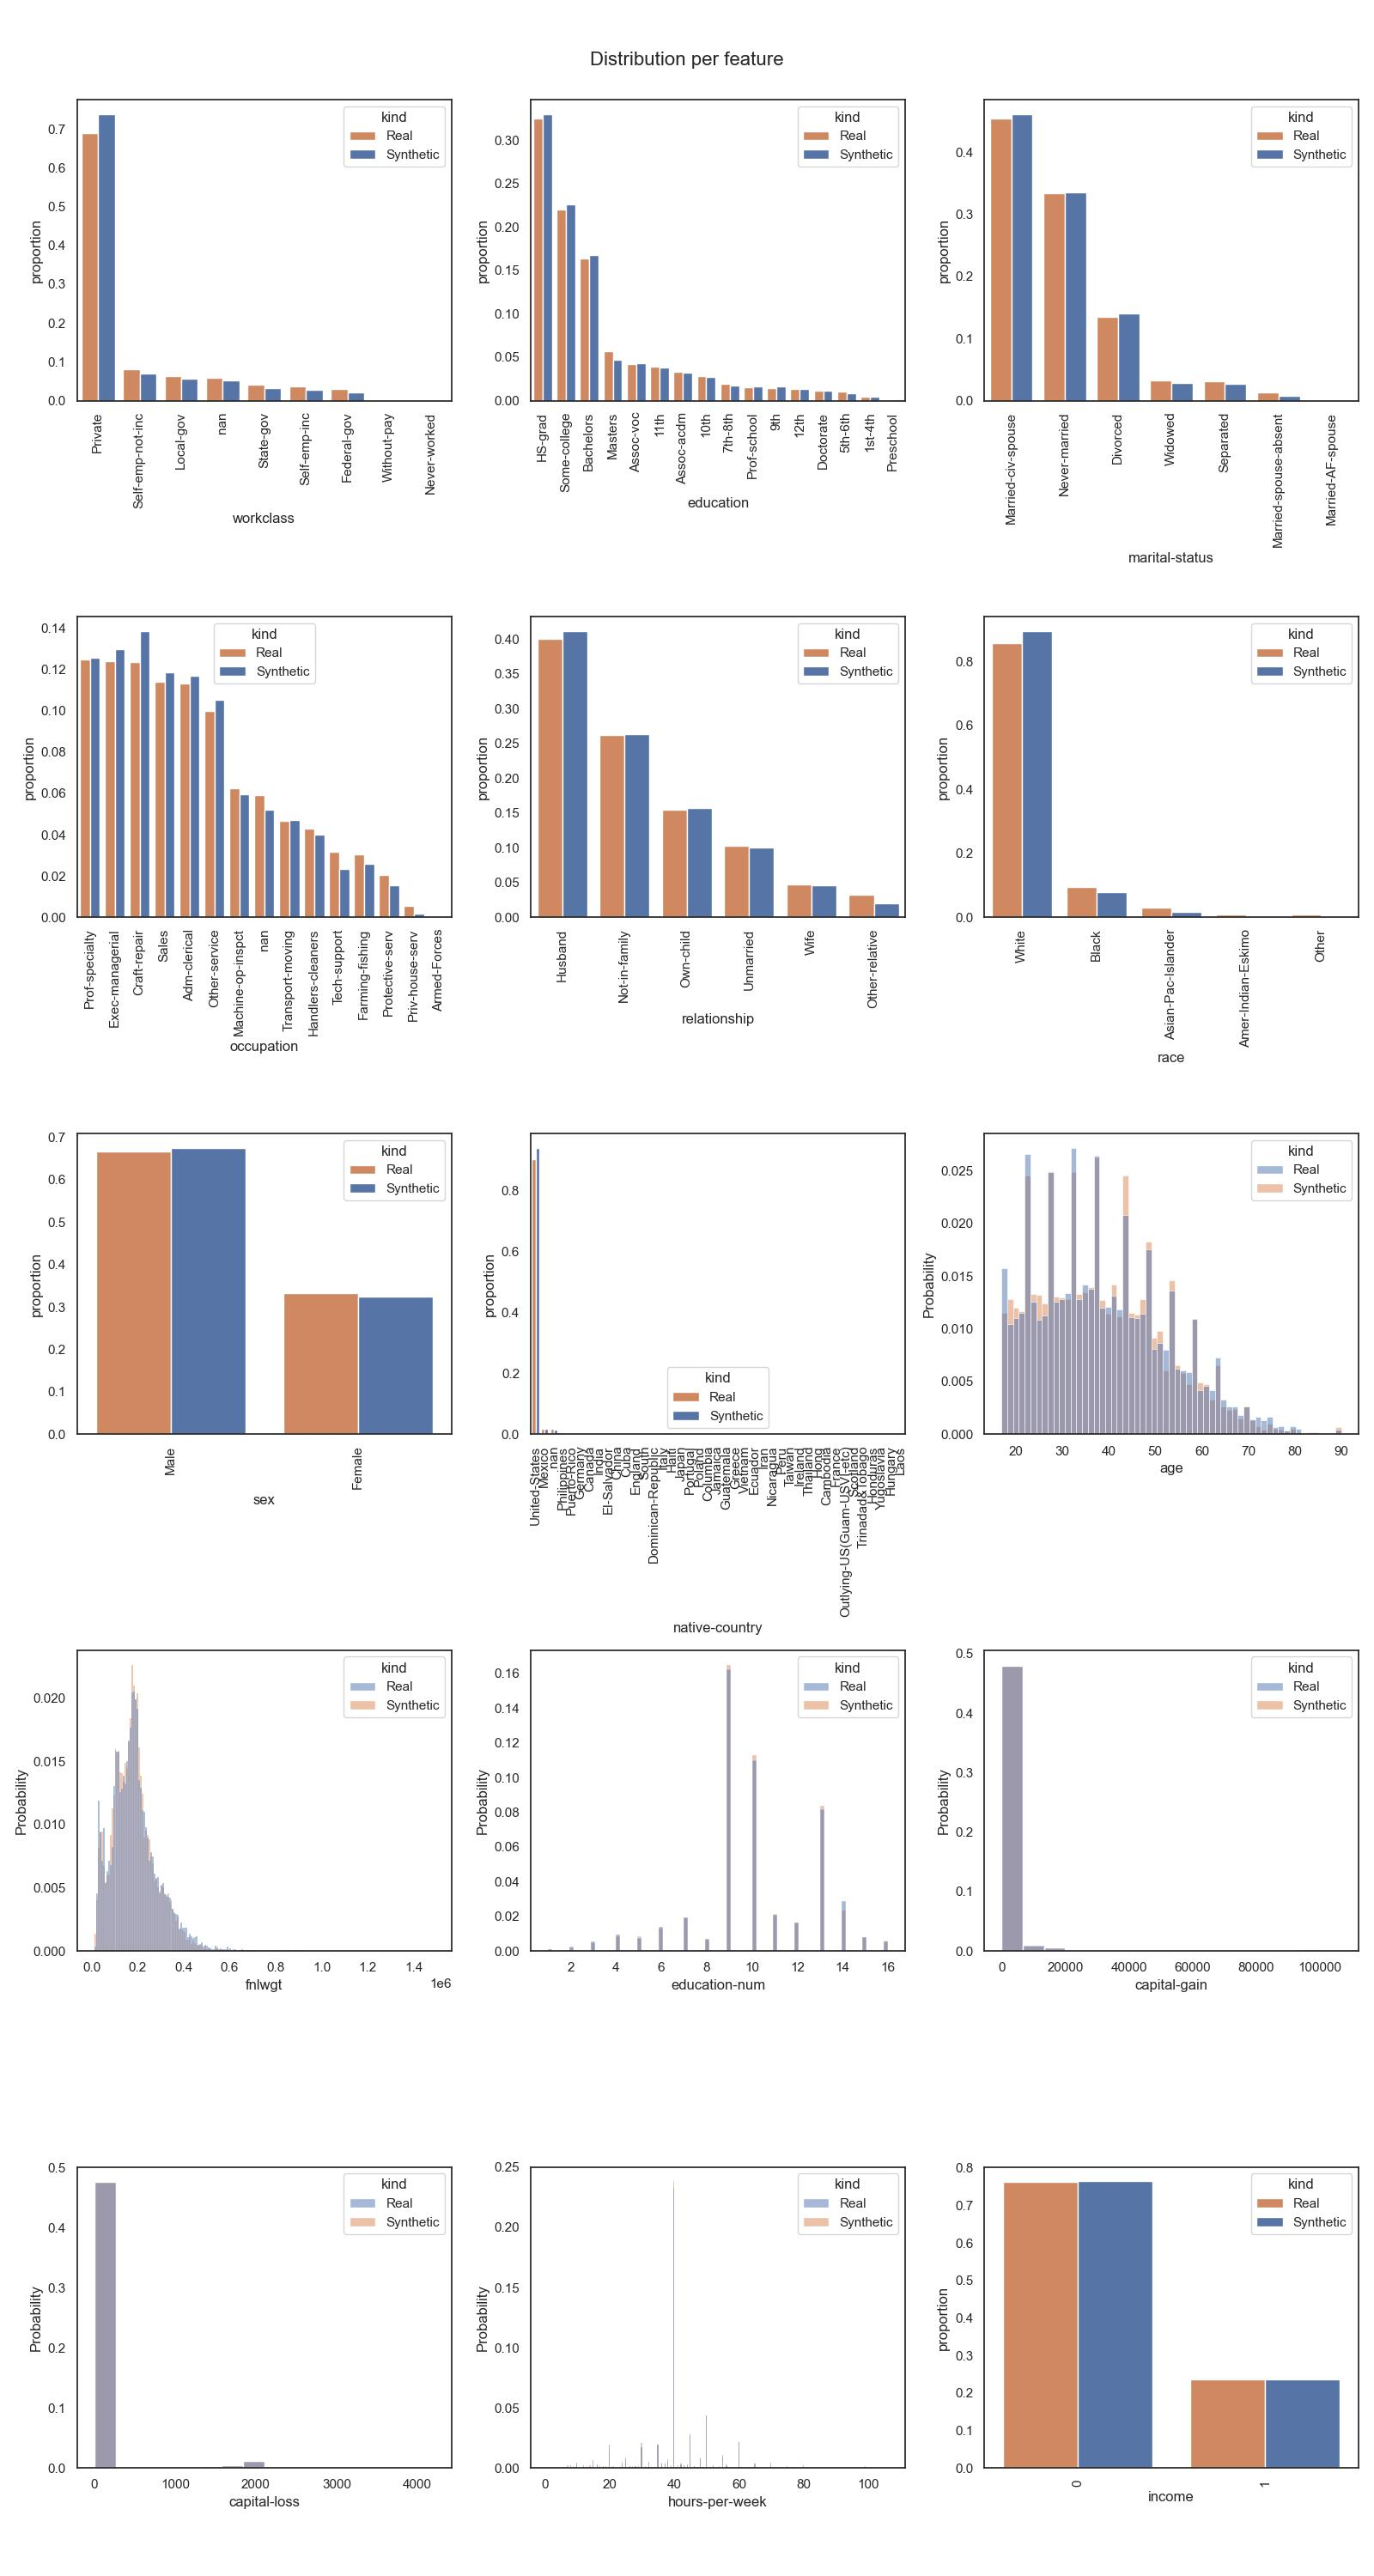
\includegraphics[height=\textheight,width=\linewidth,keepaspectratio]{images/distributions_full/tab-ddpm-bgm.jpg}
			\caption{TabDDPM-BGM$^{ml}_q$}
		\end{subfigure}
		\hfill
		\begin{subfigure}{0.3\linewidth}
			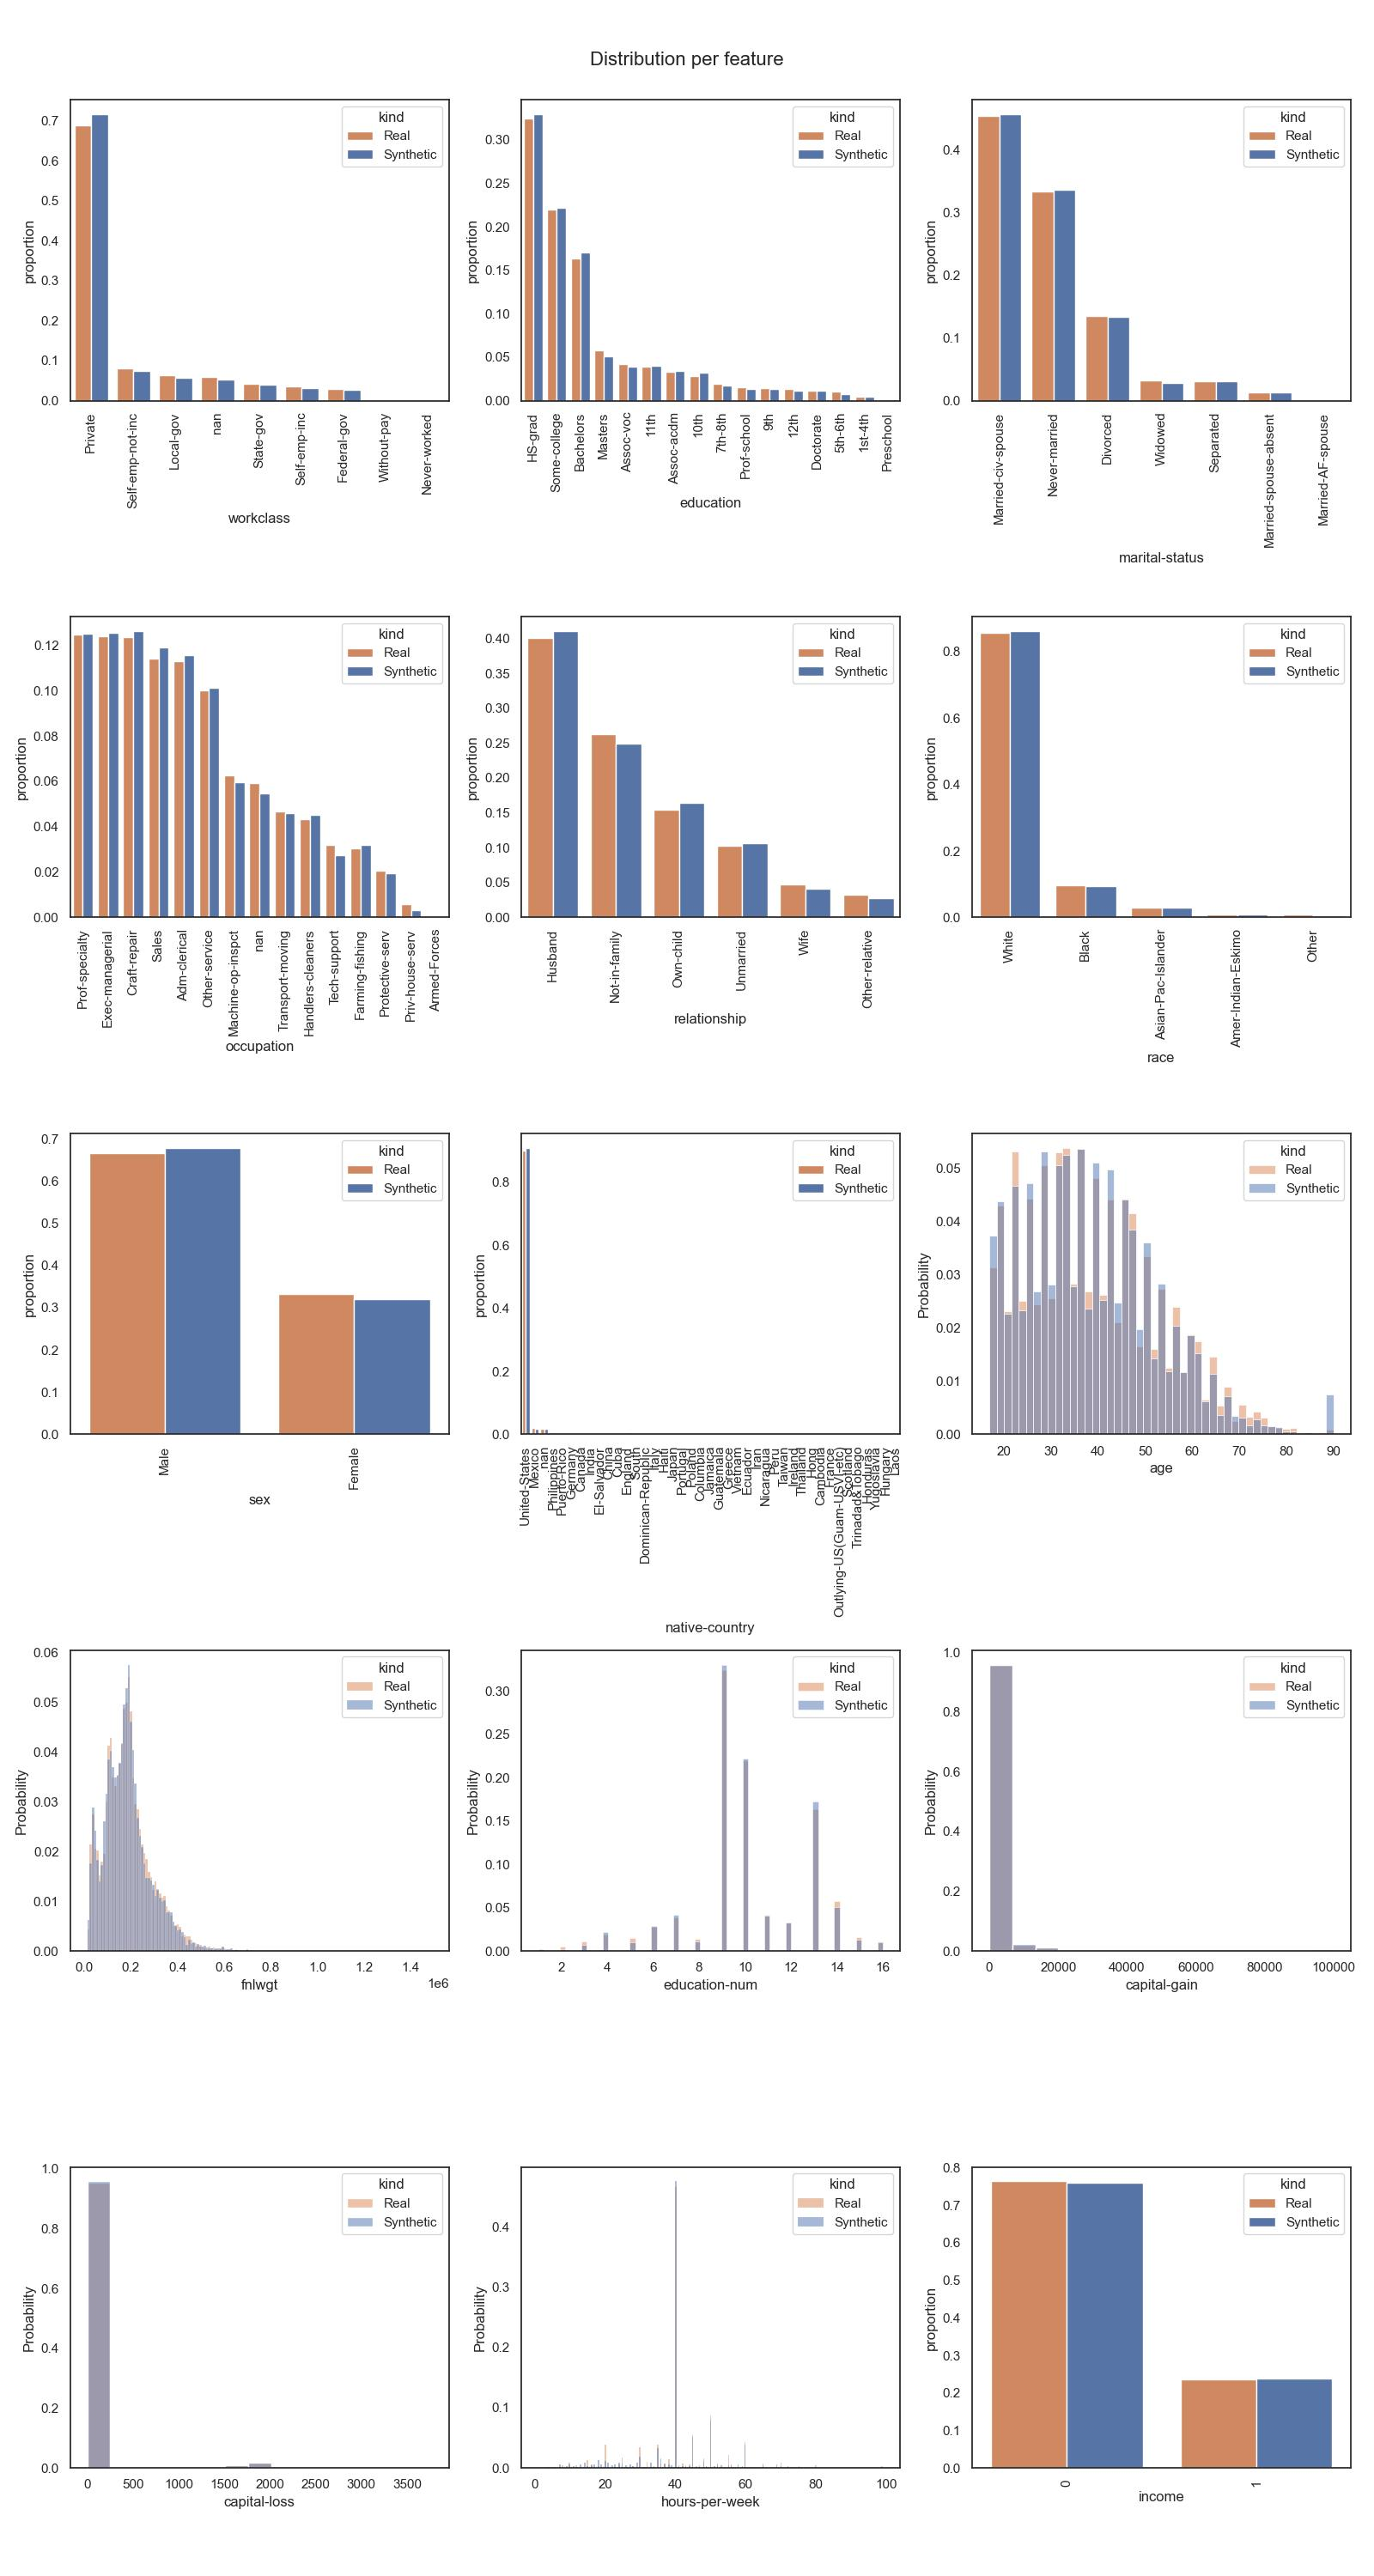
\includegraphics[height=\textheight,width=\linewidth,keepaspectratio]{images/distributions_full/tab-ddpm-bgm-simTune.jpg}
			\caption{TabDDPM-BGM$^{s}_q$}
		\end{subfigure}
		\hfill
		\begin{subfigure}{0.3\linewidth}
			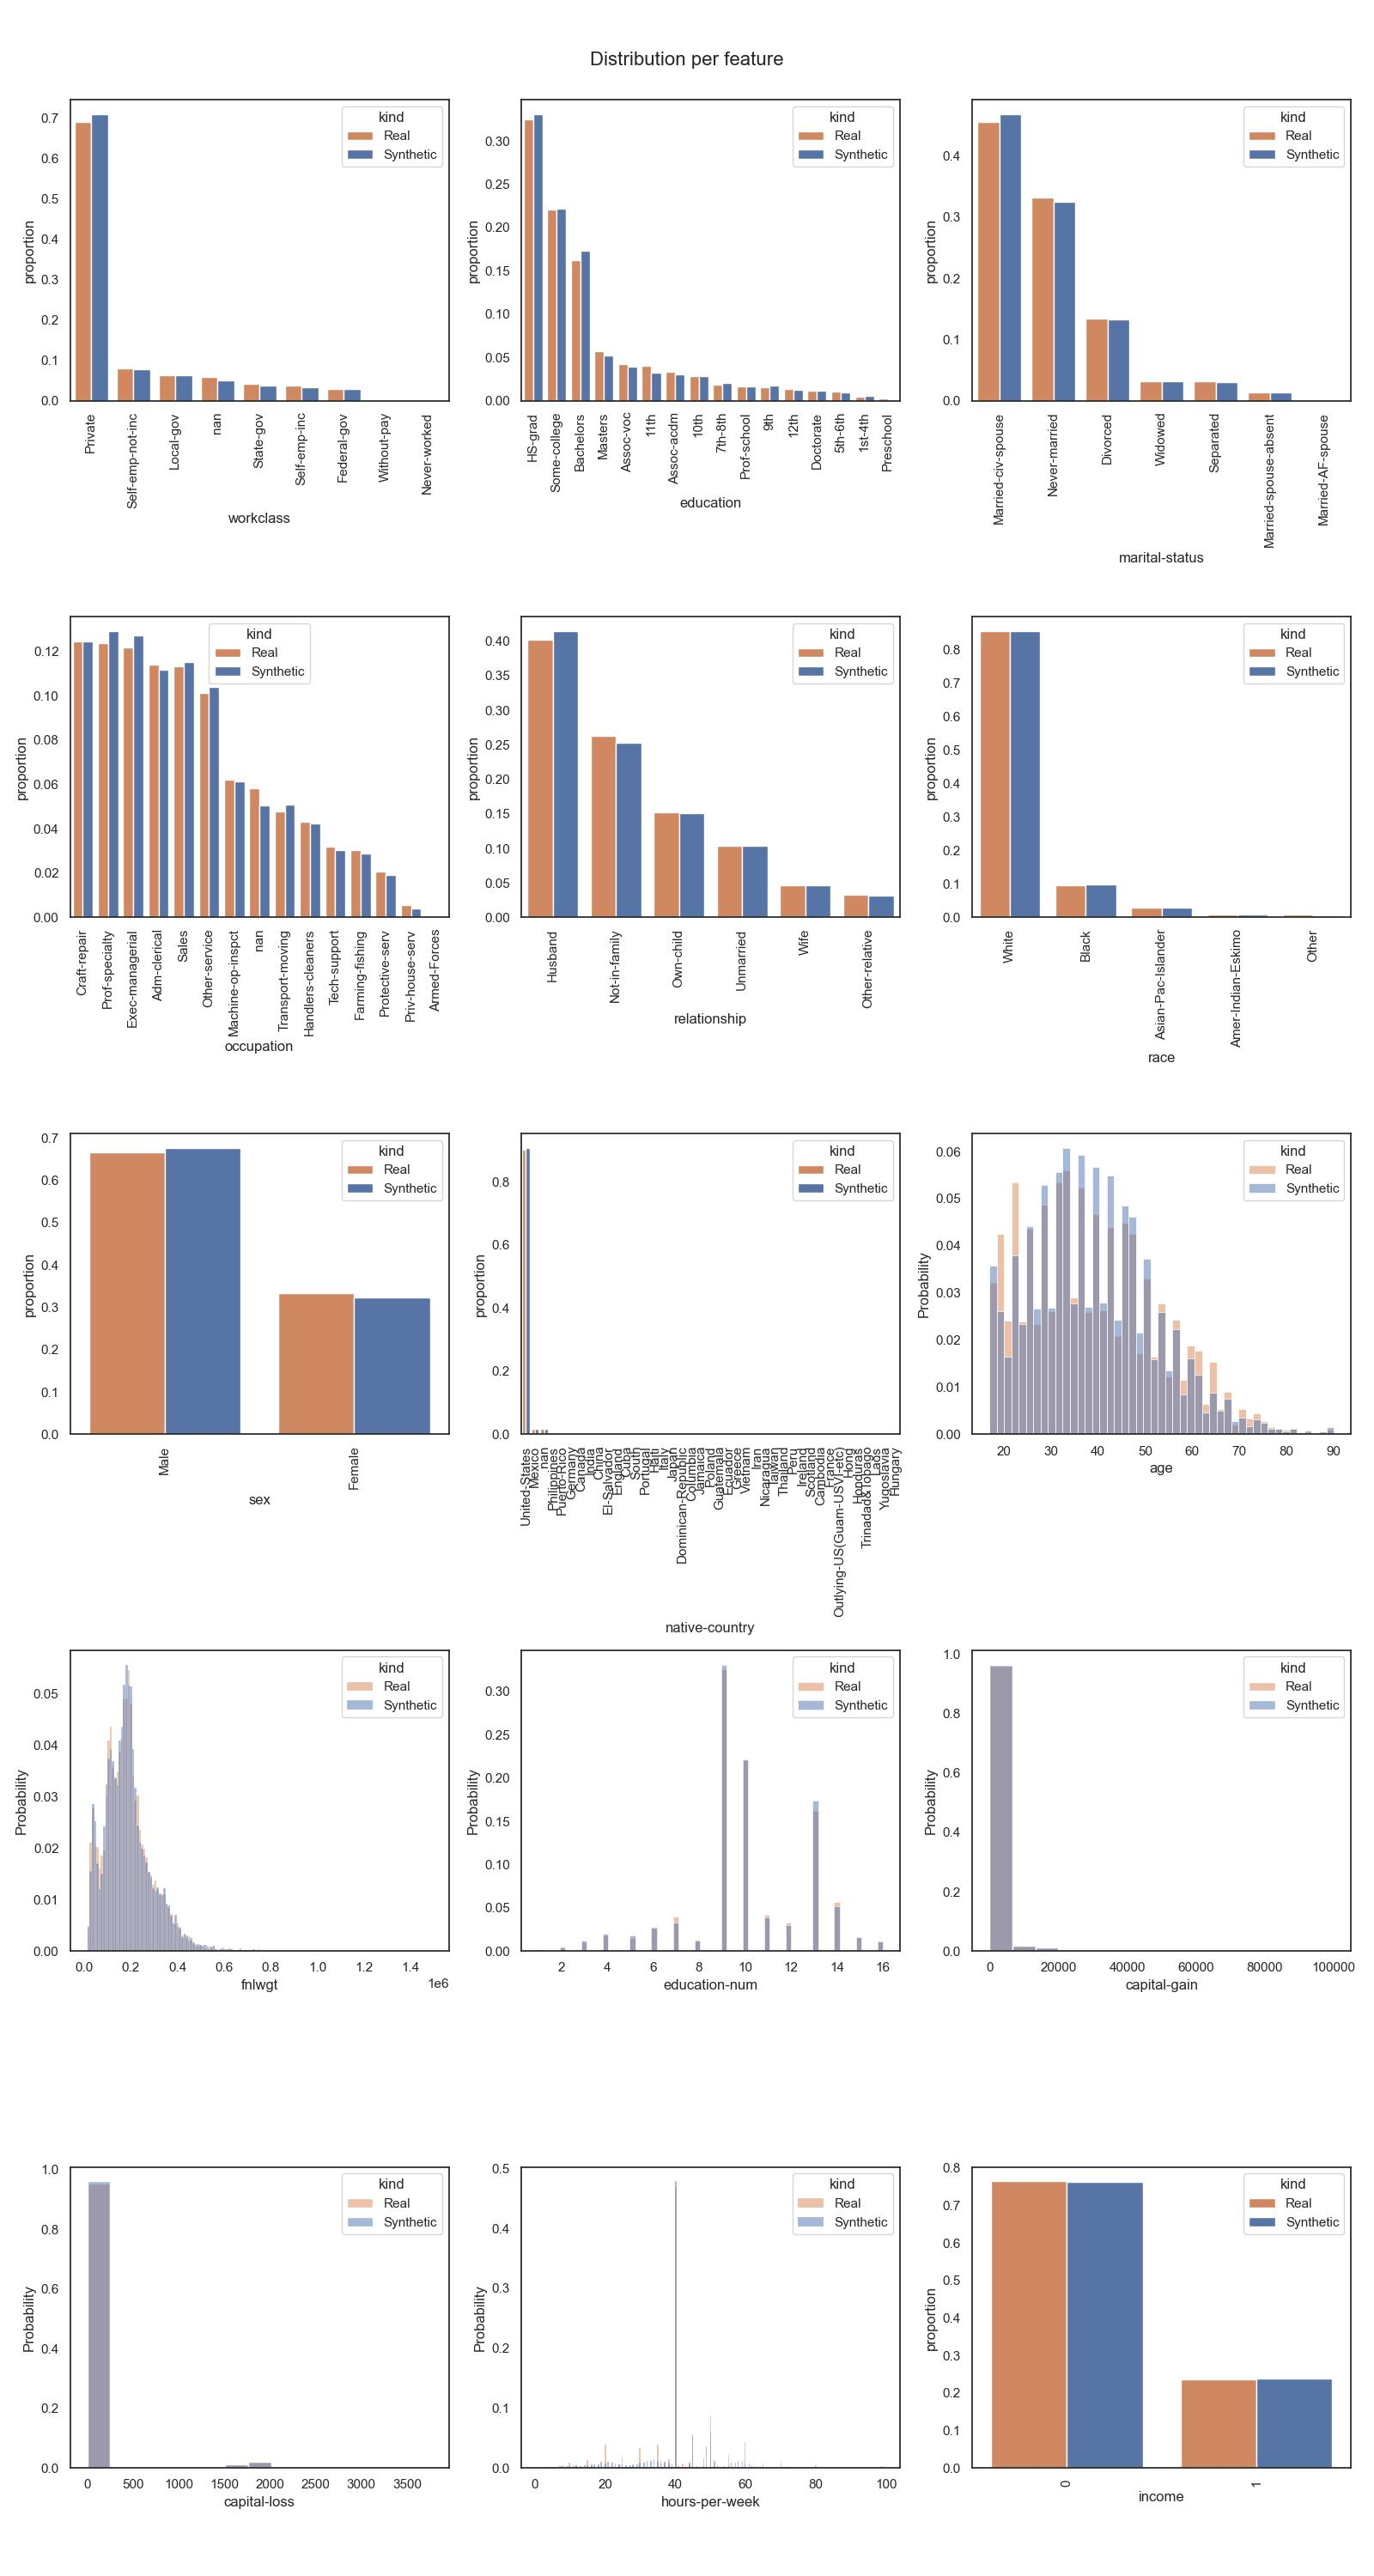
\includegraphics[height=\textheight,width=\linewidth,keepaspectratio]{images/distributions_full/tab-ddpm-bgm-simTune-minmax.jpg}
			\caption{TabDDPM-BGM$^{s}_m$}
		\end{subfigure}
		\caption[Distribution plots TabDDPM-BGM Models]{Distribution plots for TabDDPM-BGM variations}
		\label{fig_a:dist_4}
	\end{figure}
\end{landscape}
%----------
\newpage
\begin{landscape}
	\begin{figure}[h]
		\centering
		\hfill
		\begin{subfigure}{0.3\linewidth}
			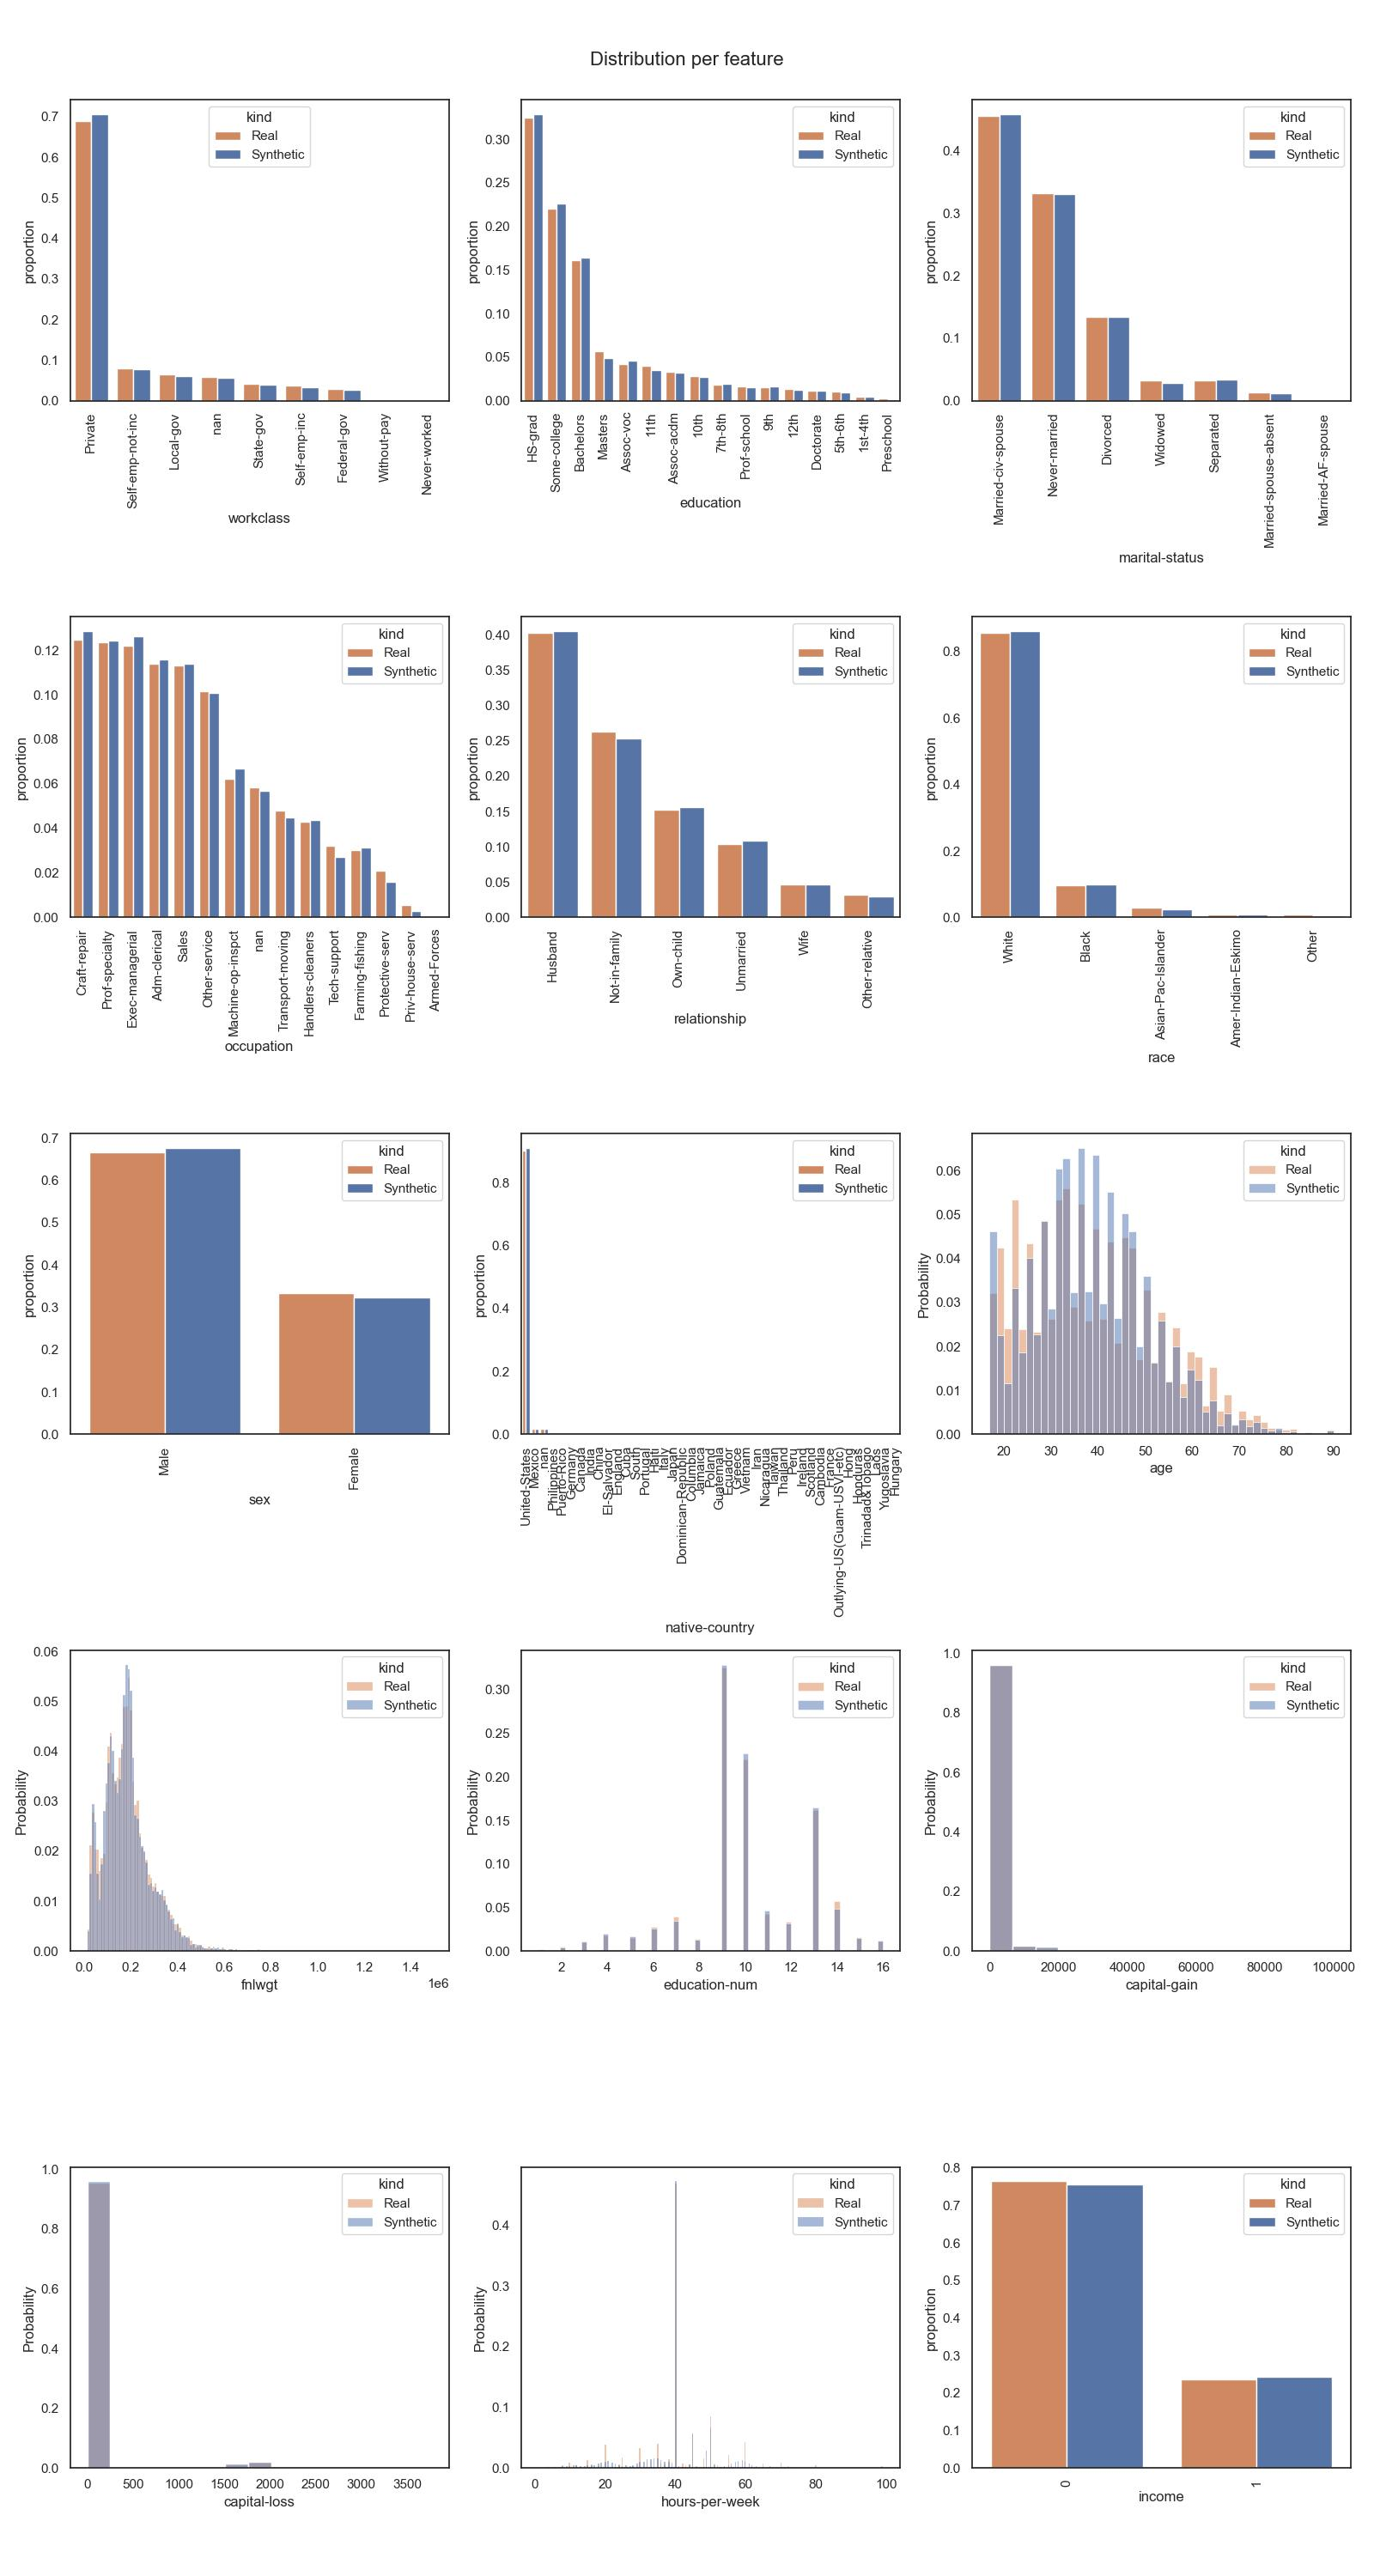
\includegraphics[height=\textheight,width=\linewidth,keepaspectratio]{images/distributions_full/tab-ddpm-bgm-simTune-none.jpg}
			\caption{TabDDPM-BGM$^{s}_n$}
		\end{subfigure}
		\hfill
		\begin{subfigure}{0.3\linewidth}
			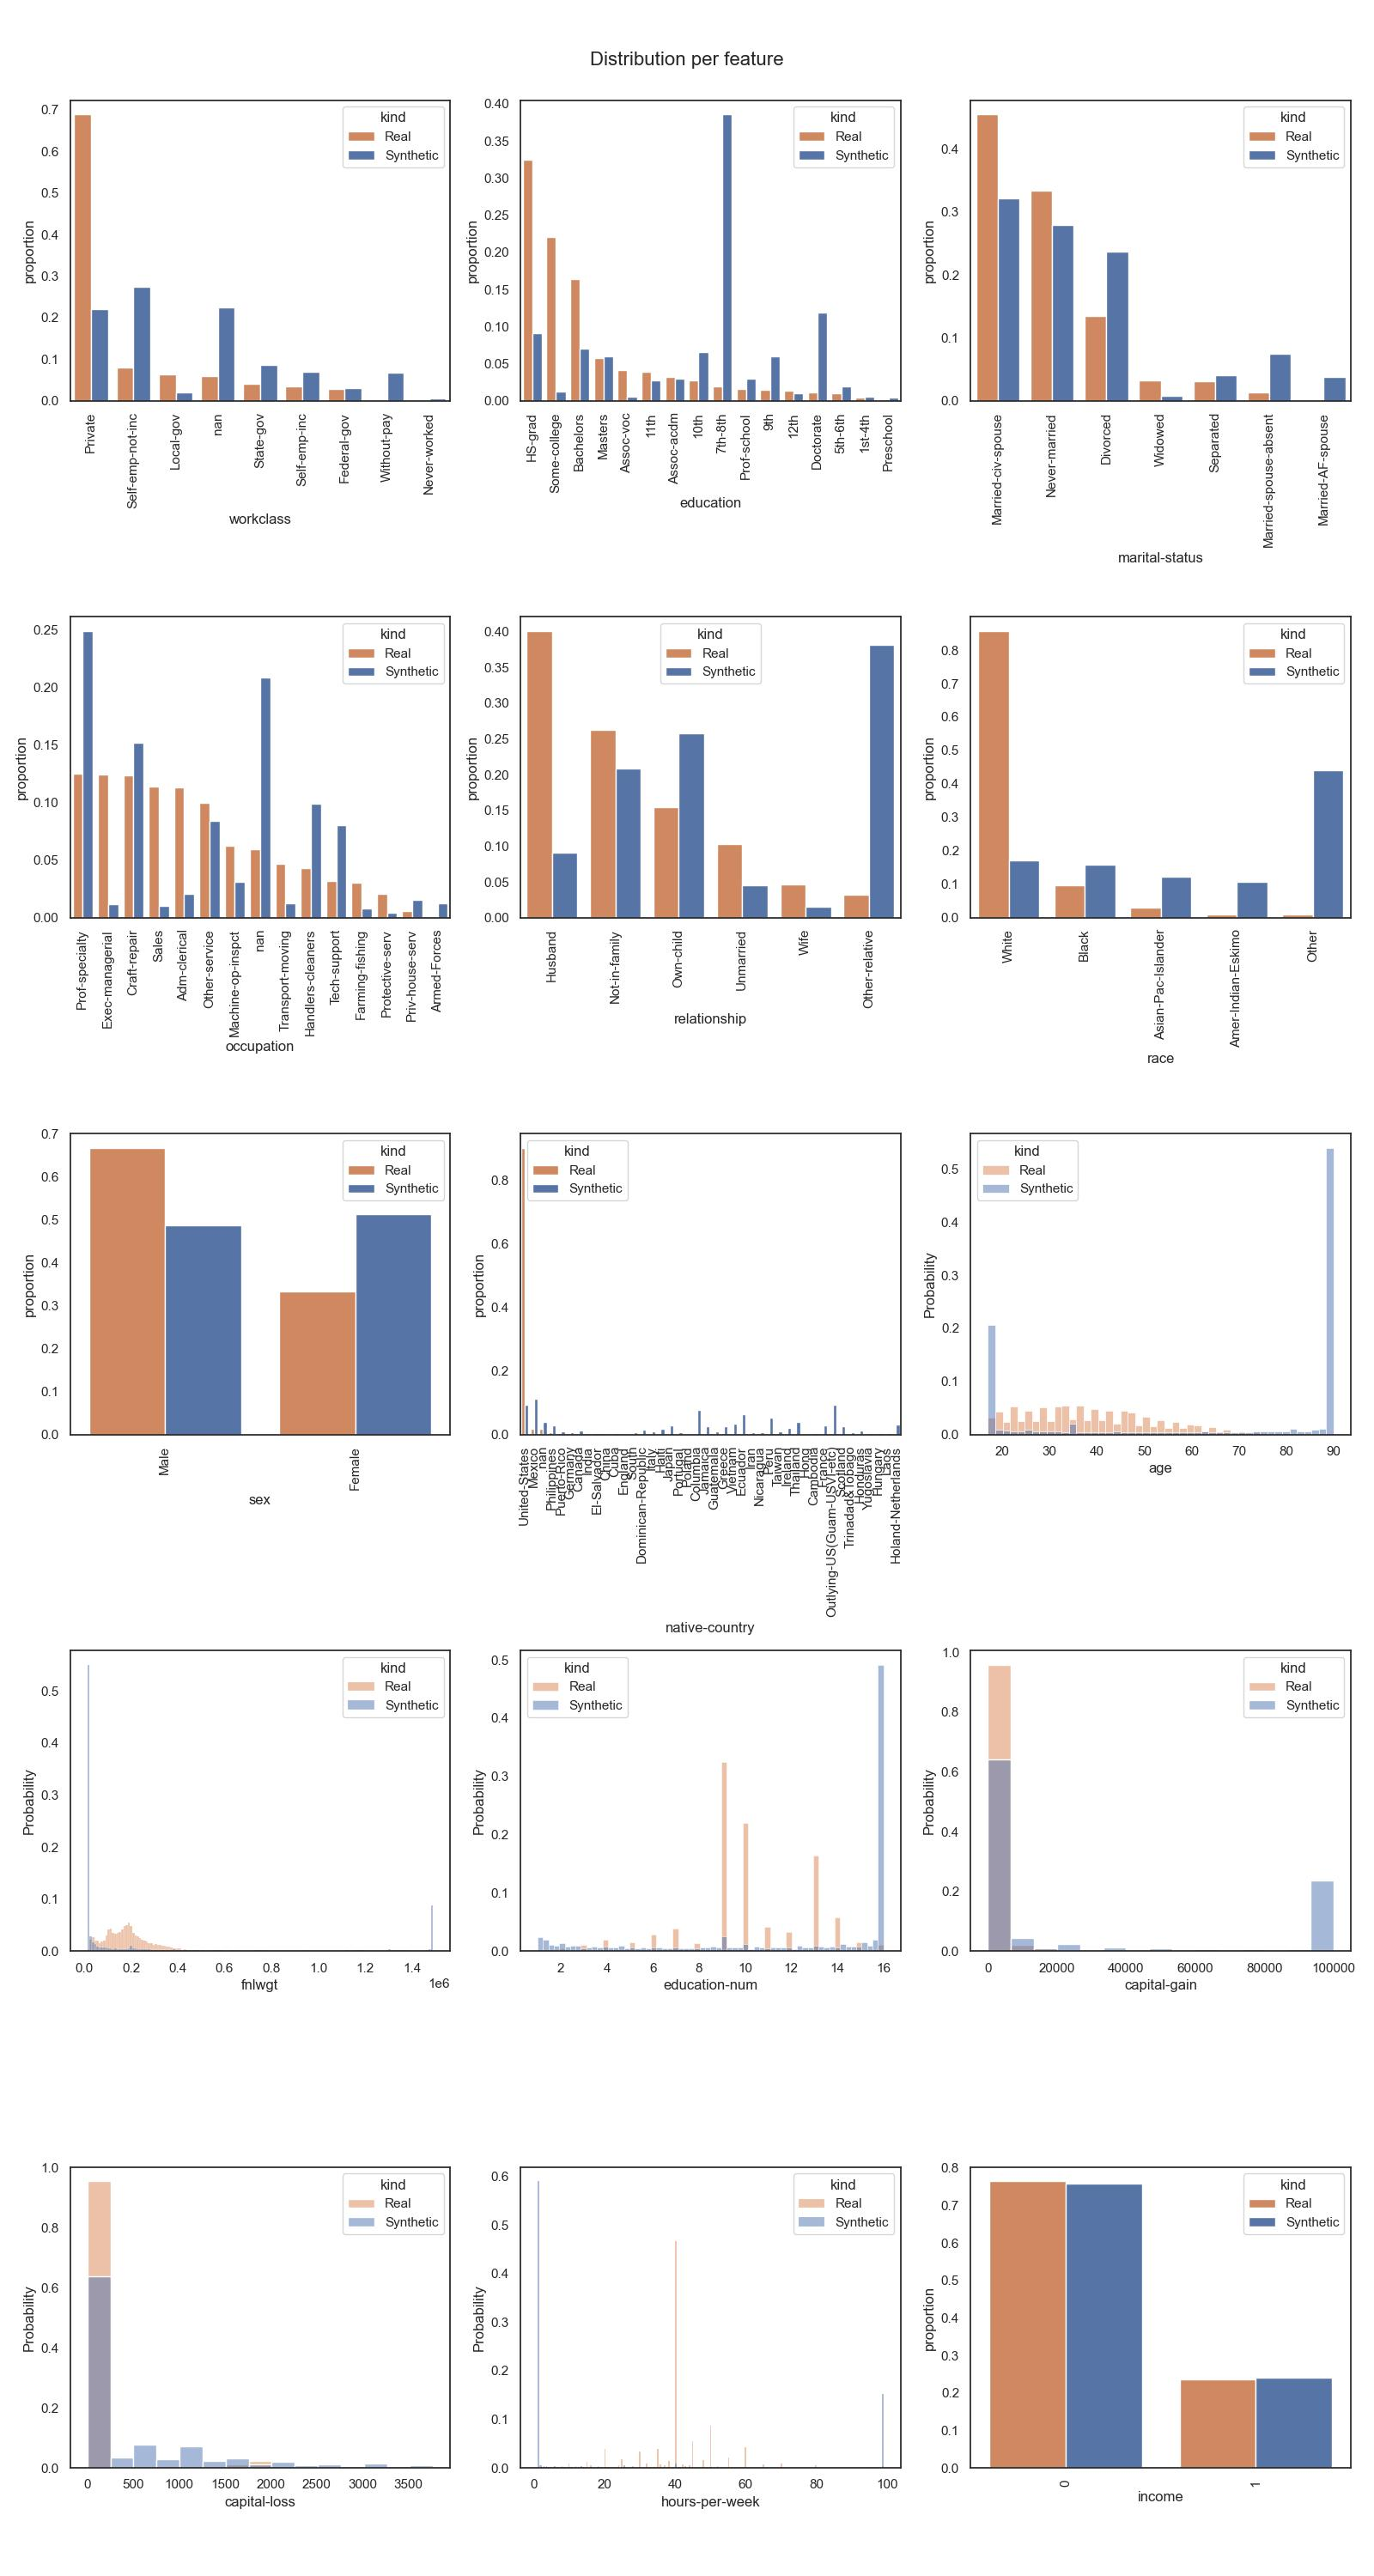
\includegraphics[height=\textheight,width=\linewidth,keepaspectratio]{images/distributions_full/tab-ddpm-ft.jpg}
			\caption{TabDDPM-FT$^{ml}_q$}
		\end{subfigure}
		\hfill
		\begin{subfigure}{0.3\linewidth}
			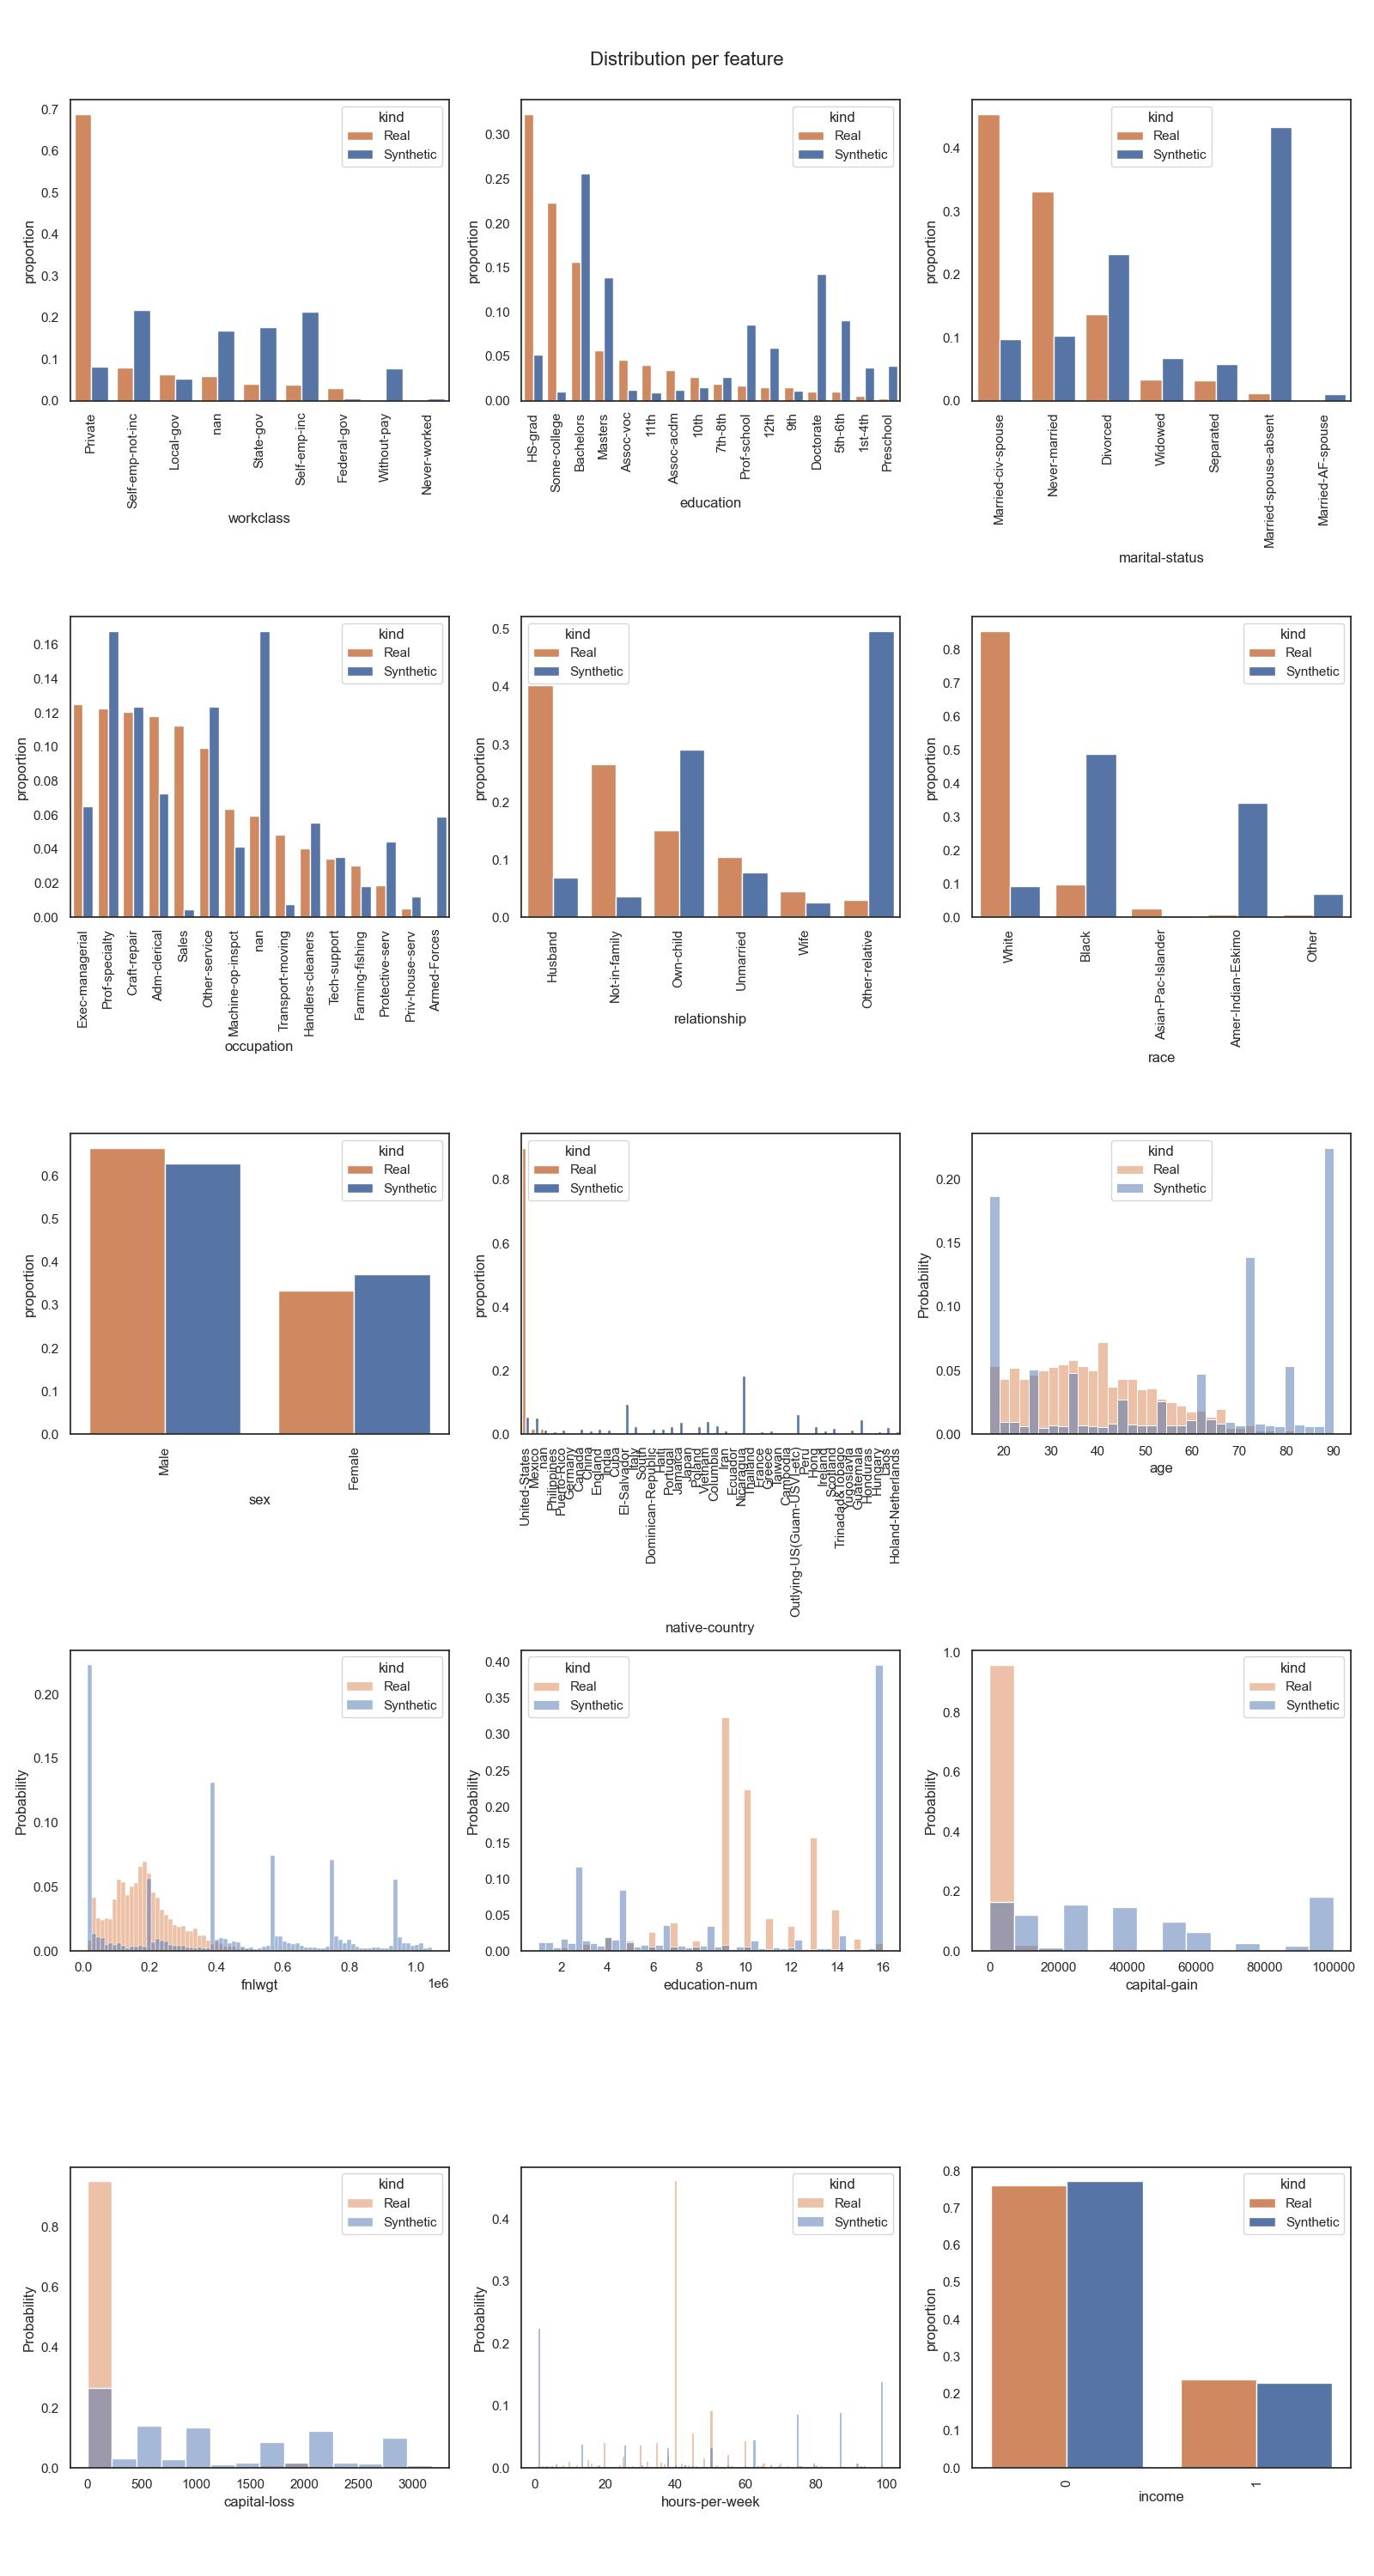
\includegraphics[height=\textheight,width=\linewidth,keepaspectratio]{images/distributions_full/tab-ddpm-ft-simTune.jpg}
			\caption{TabDDPM-FT$^{ml}_q$}
		\end{subfigure}
		\caption[Distribution plots TabDDPM-FT and -BGM Models]{Distribution plots for TabDDPM-FT variations}
		\label{fig_a:dist_5}
	\end{figure}
\end{landscape}



%-------------

\newpage
\subsection[]{Cumulative Distribution Plots}
\label{A:cumsum}
\begin{figure}[h]
	\centering
	\begin{subfigure}{0.6\textwidth}
		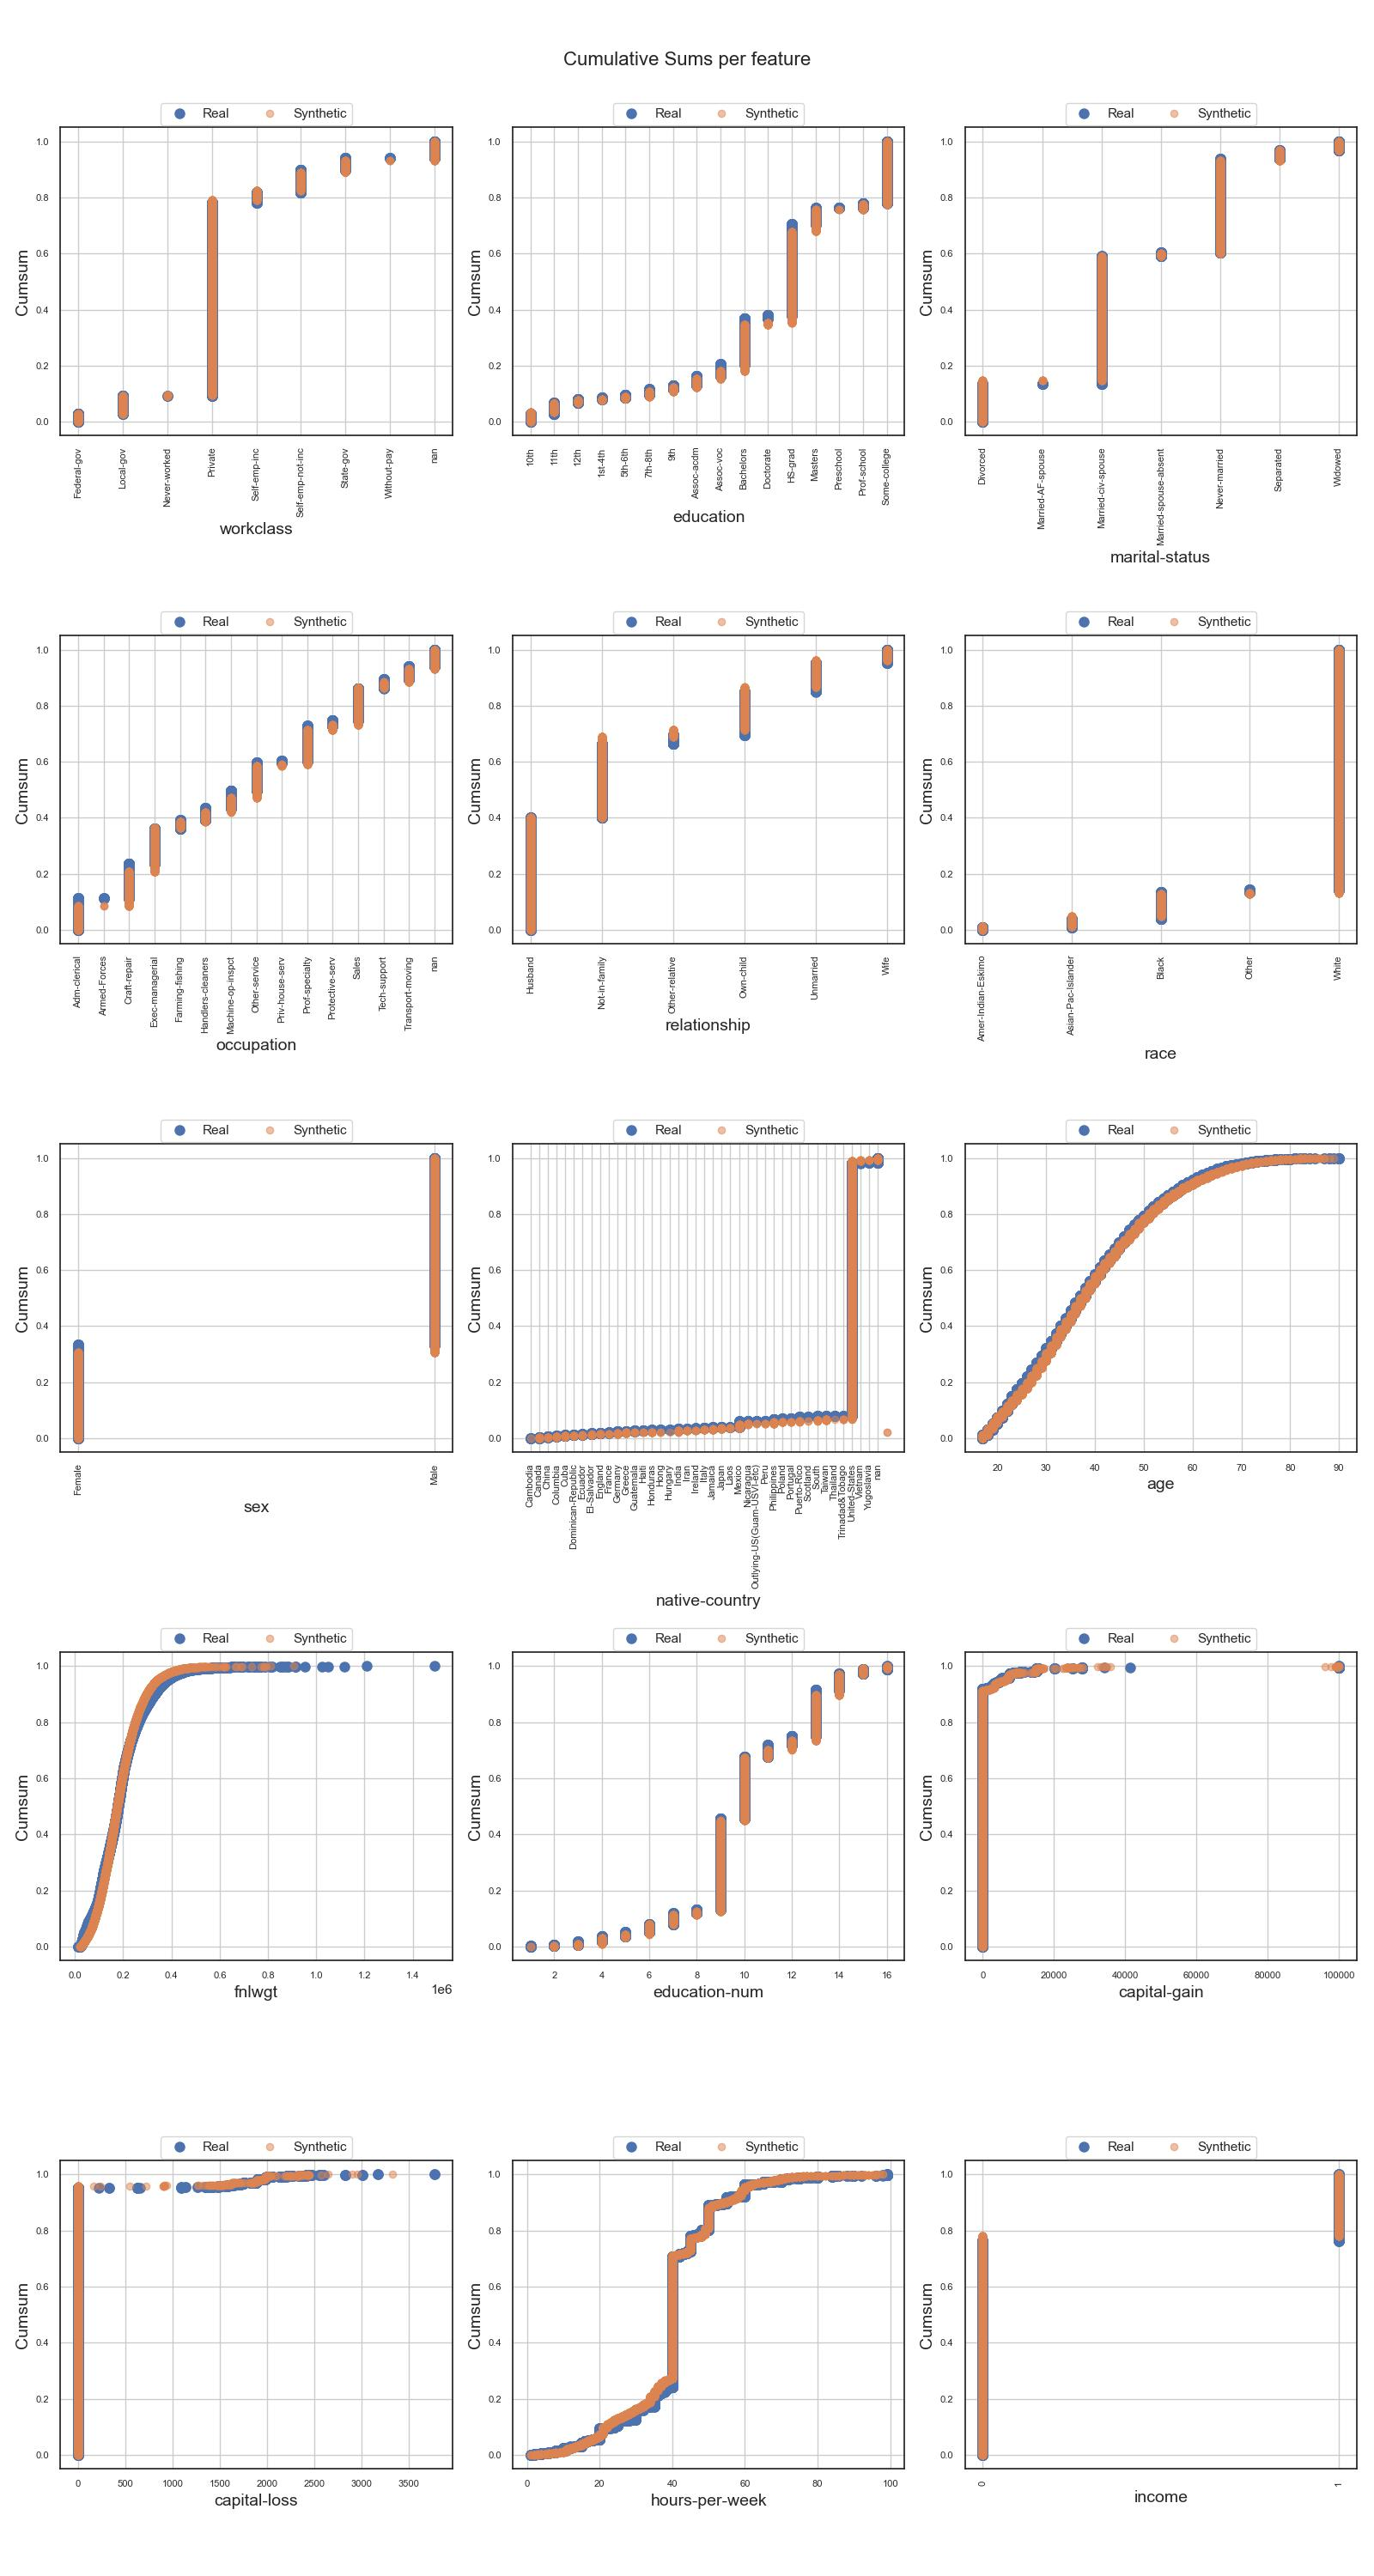
\includegraphics[width=\linewidth]{images/cumsums/ctabgan+.jpg}
		\caption{CTABGAN+$^{ml}$}
	\end{subfigure}
	\caption[Cumulative Distribution plots CTABGAN+ Model]{Cumulative Distribution plots for CTABGAN+$^{ml}$}
	\label{fig_a:cumsum_0}
\end{figure}


\begin{landscape}
	\begin{figure}[h]
		\centering
		\hfill
		\begin{subfigure}{0.3\linewidth}
			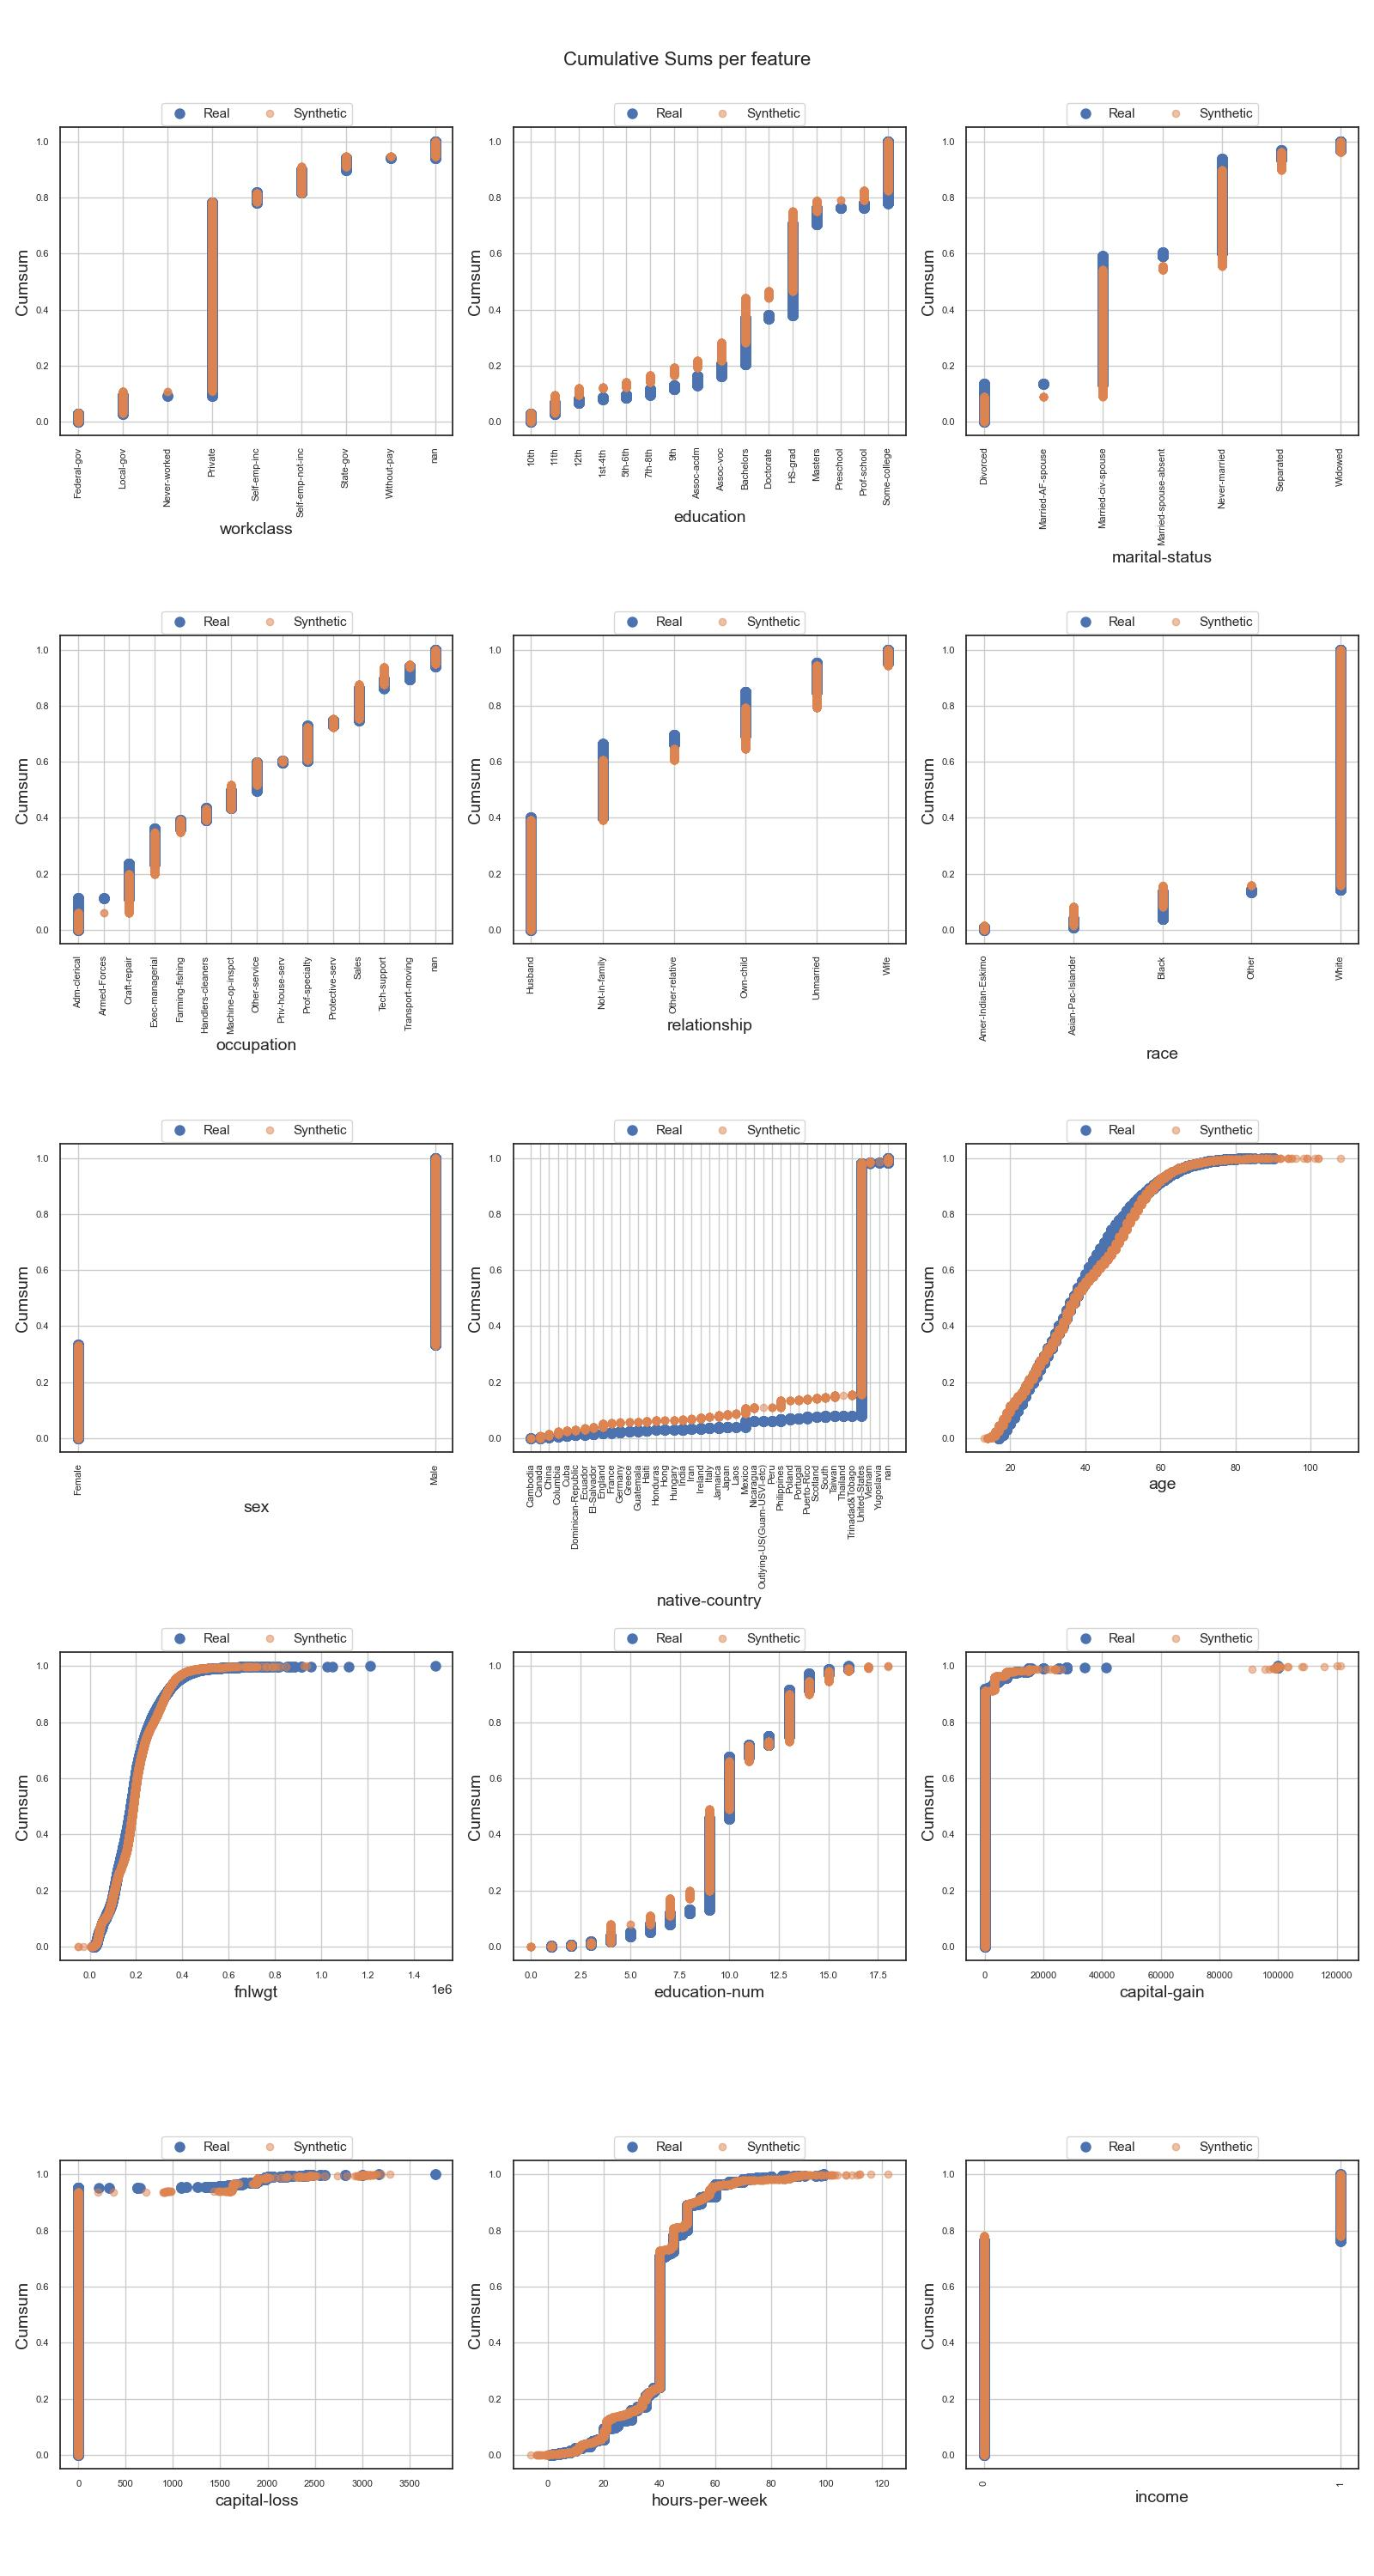
\includegraphics[height=\textheight,width=\linewidth,keepaspectratio]{images/cumsums/ctabgan.jpg}
			\caption{CTABGAN$^{ml}$}
		\end{subfigure}
		\hfill
		\begin{subfigure}{0.3\linewidth}
			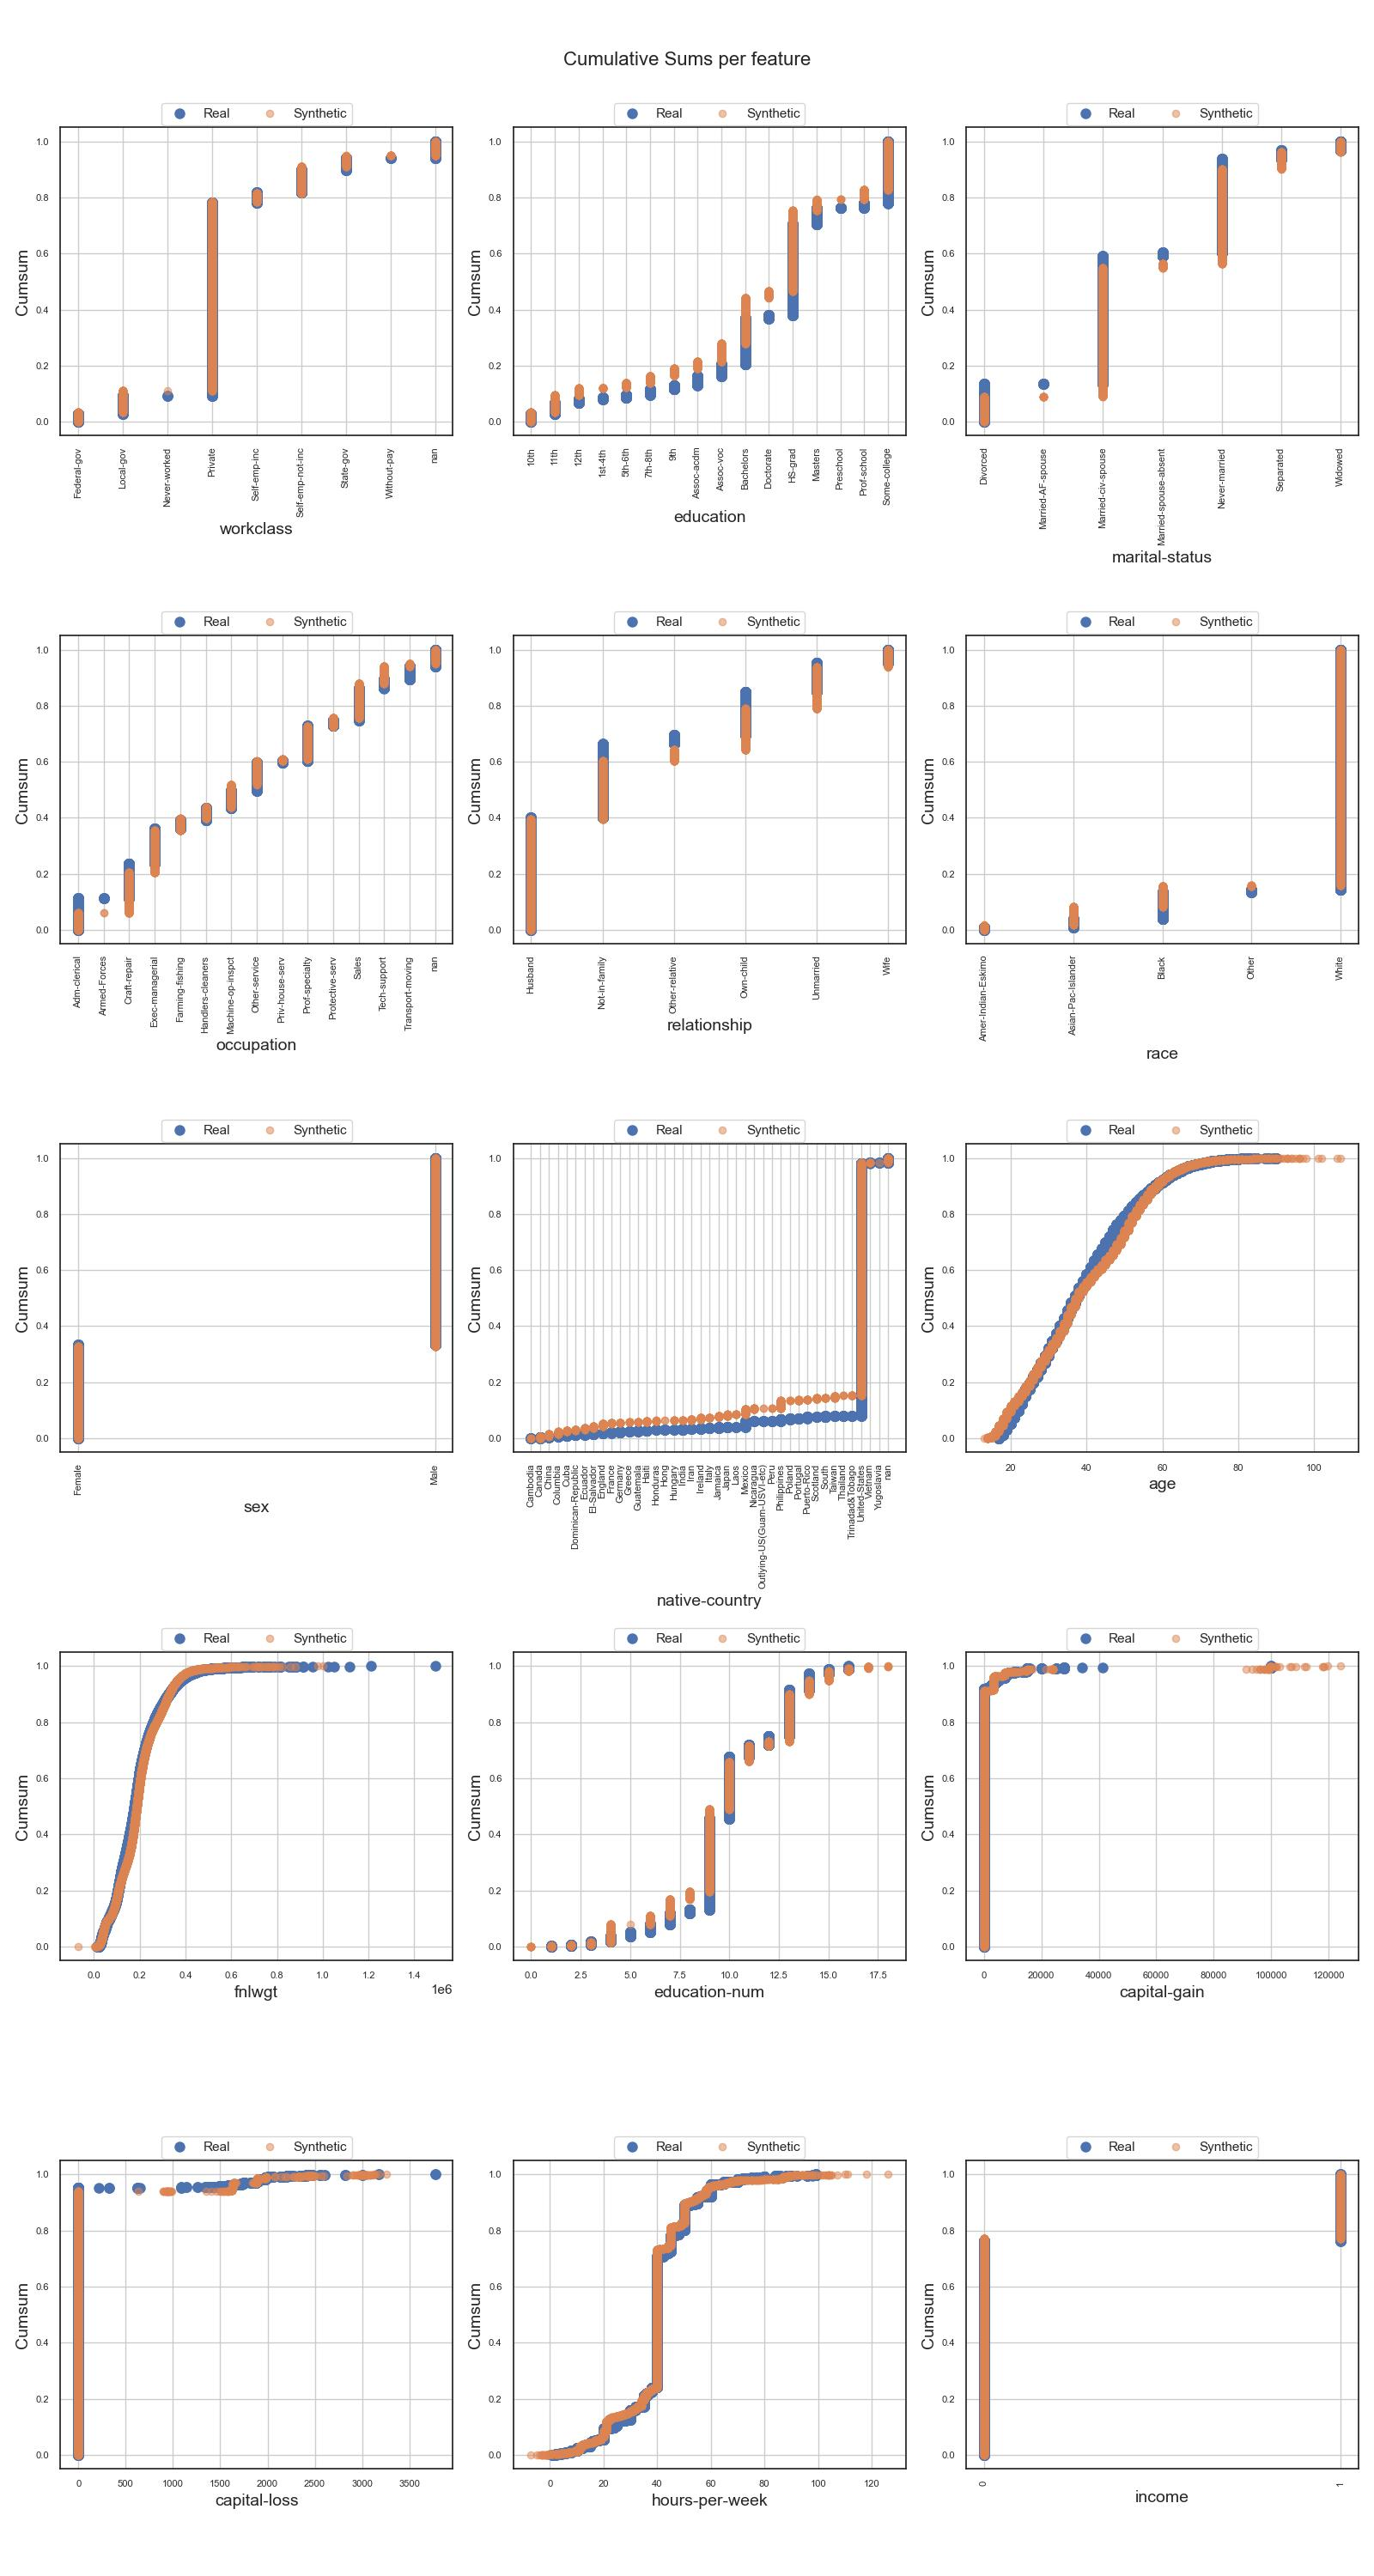
\includegraphics[height=\textheight,width=\linewidth,keepaspectratio]{images/cumsums/ctabgan_simTune.jpg}
			\caption{CTABGAN$^s$}
		\end{subfigure}	
		\hfill
		\begin{subfigure}{0.3\linewidth}
			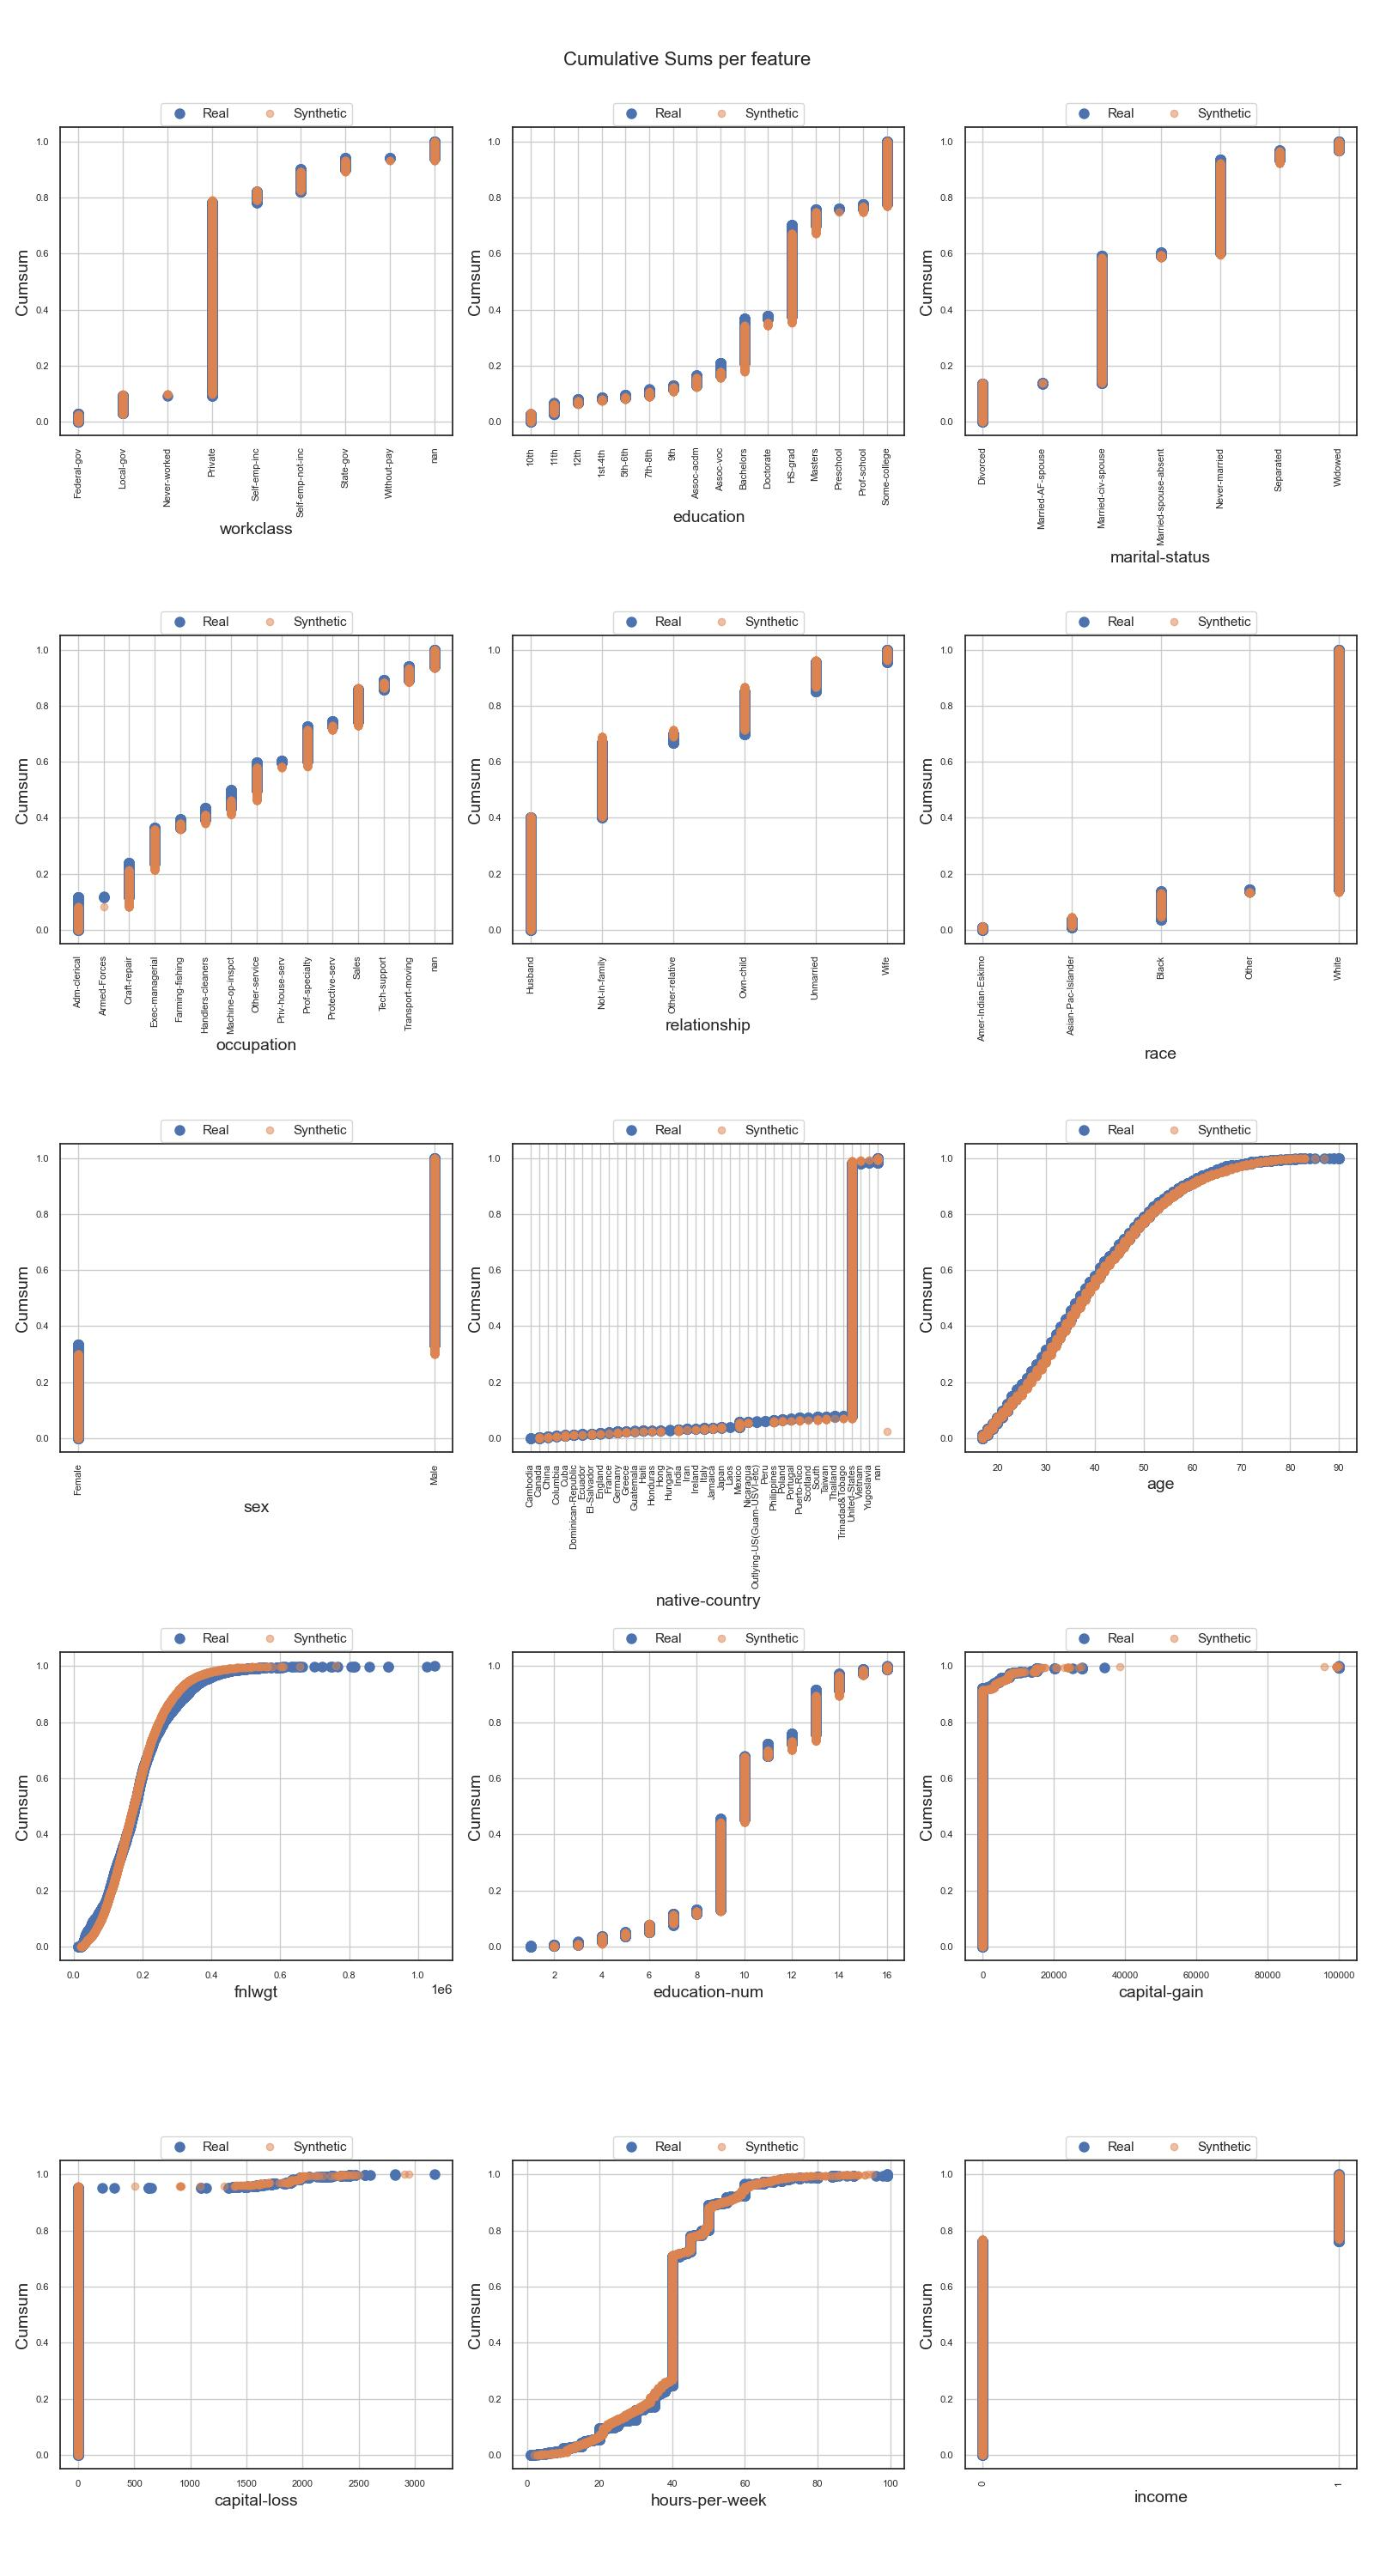
\includegraphics[height=\textheight,width=\linewidth,keepaspectratio]{images/cumsums/ctabgan+_simTune.jpg}
			\caption{CTABGAN+$^s$}
		\end{subfigure}	
		\hfill
		\caption[Cumulative Distribution plots CTABGAN Models]{Cumulative Distribution plots for CTABGAN$^{ml}$, CTABGAN$^s$ and CTABGAN+$^s$}
		\label{fig_a:cumsum_1}
	\end{figure}
\end{landscape}
%----------
\newpage
\begin{landscape}
	\begin{figure}[h]
		\centering
		\hfill
		\begin{subfigure}{0.3\linewidth}
			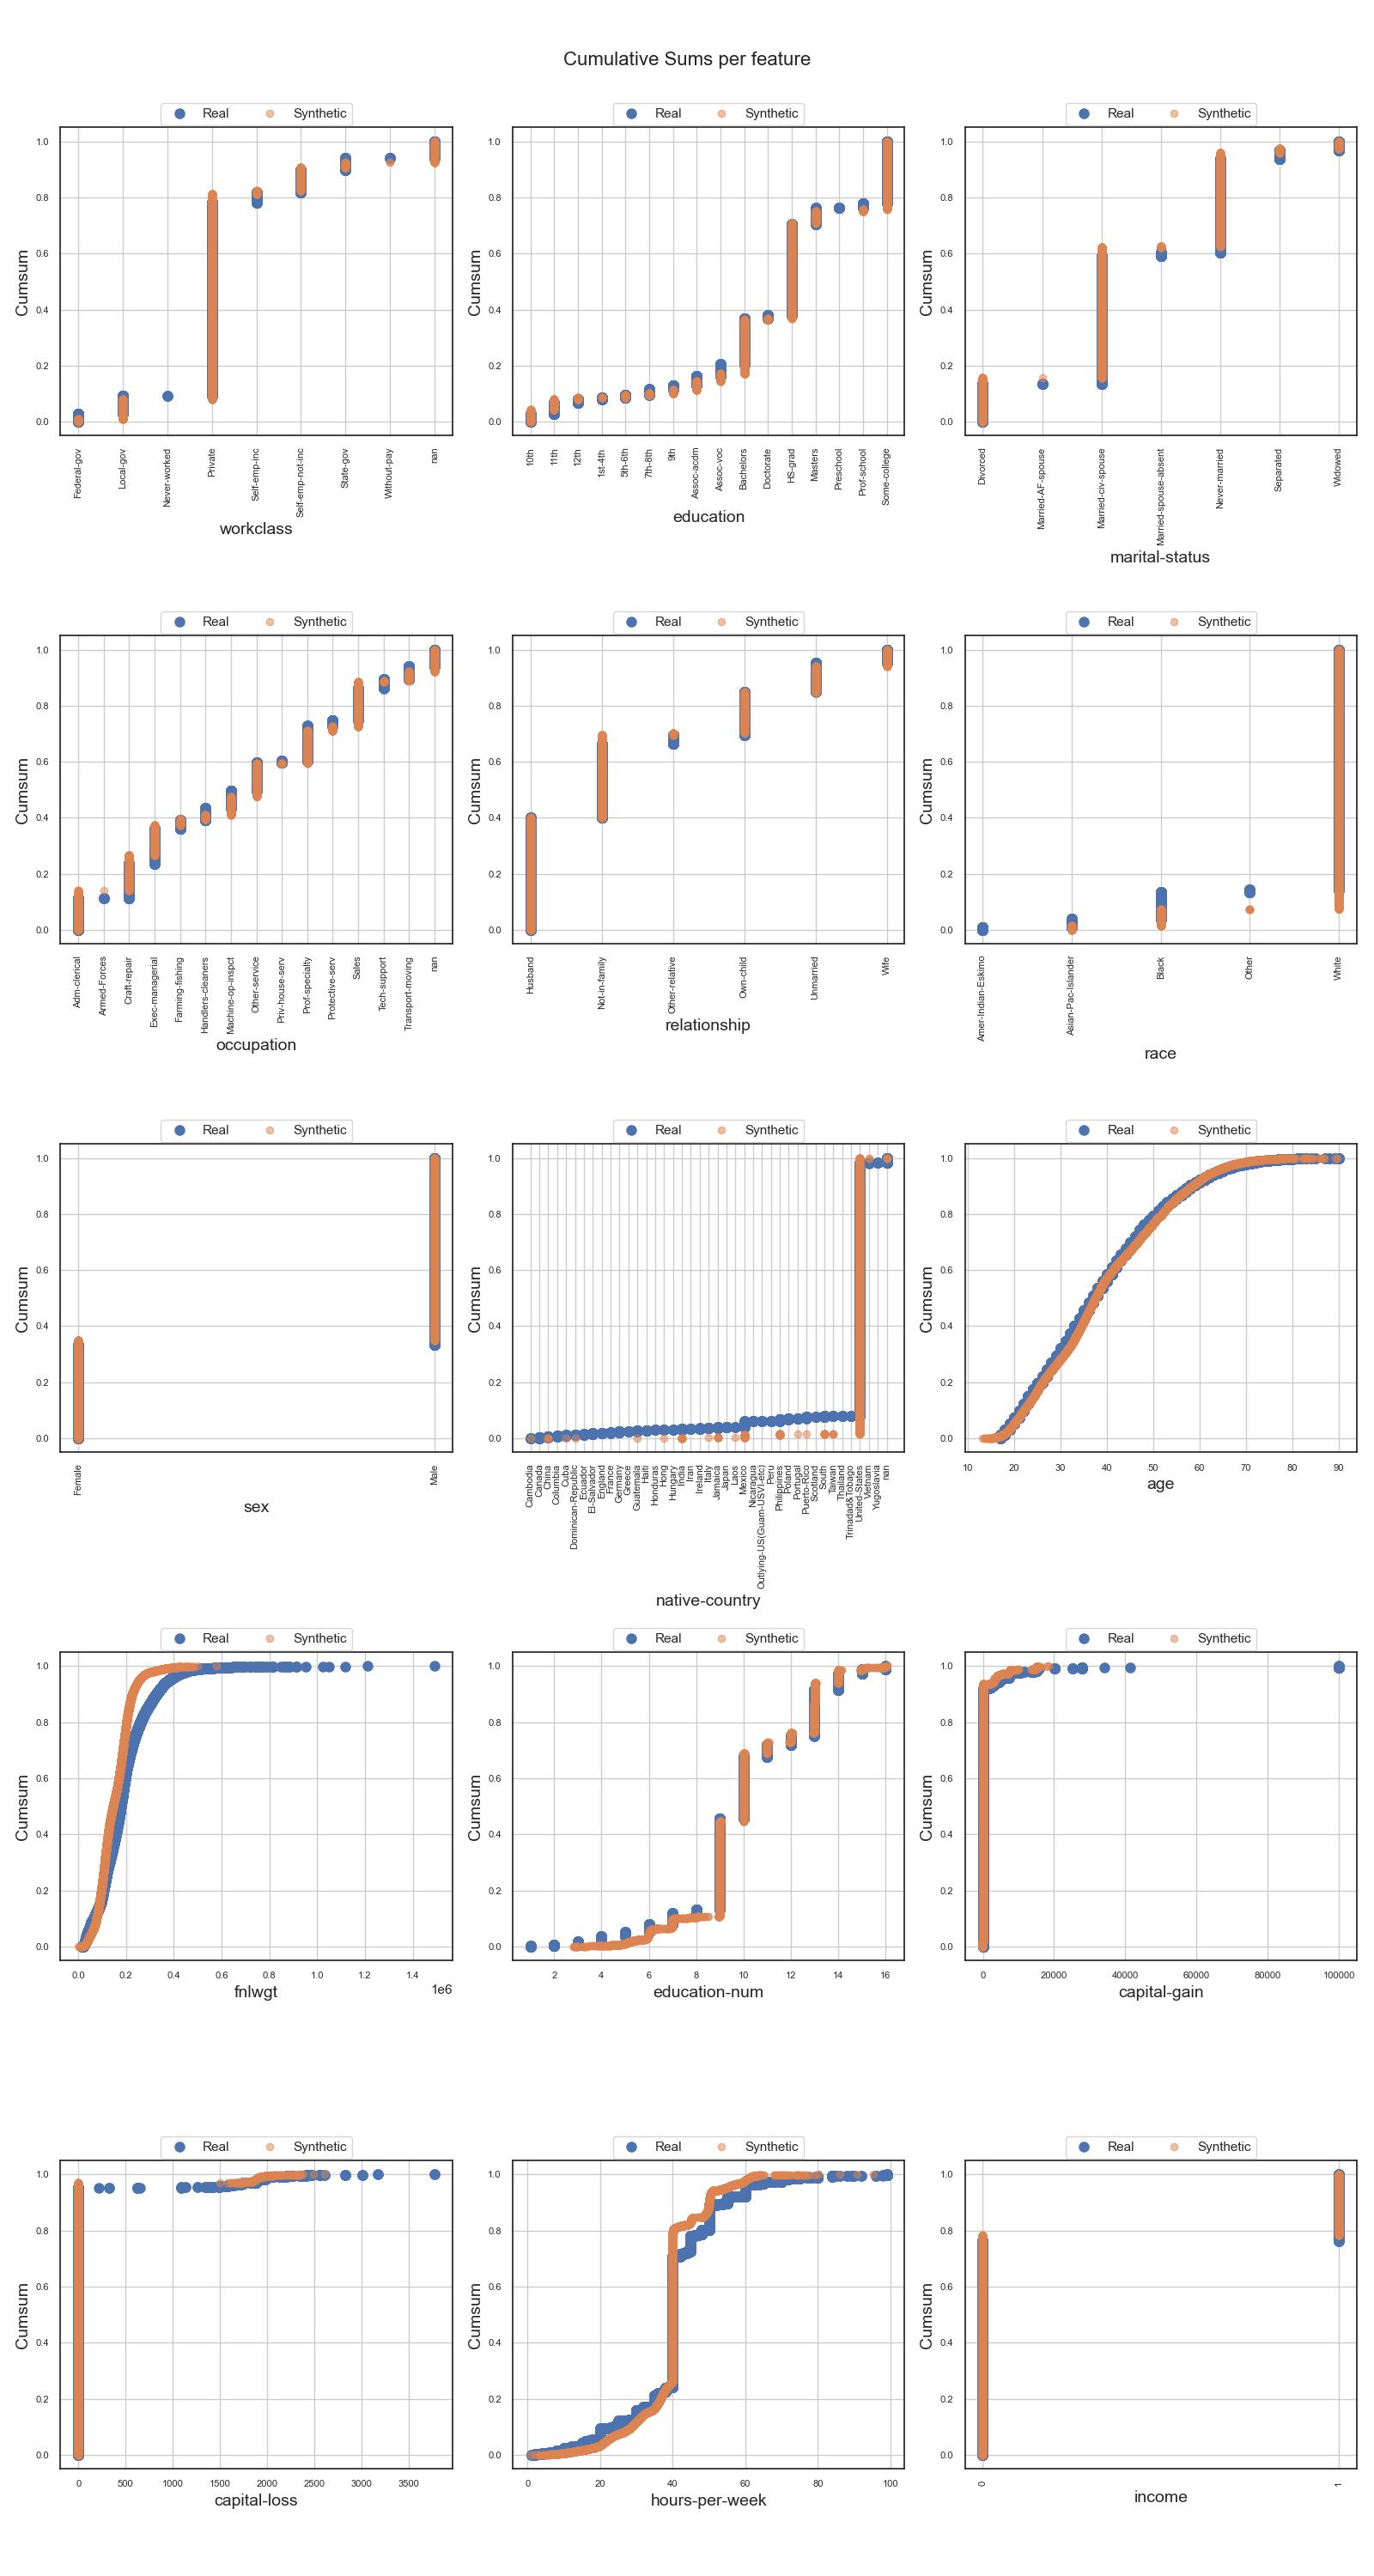
\includegraphics[height=\textheight,width=\linewidth,keepaspectratio]{images/cumsums/tvae.jpg}
			\caption{TVAE$^{ml}$}
		\end{subfigure}		
		\hfill
		\begin{subfigure}{0.3\linewidth}
			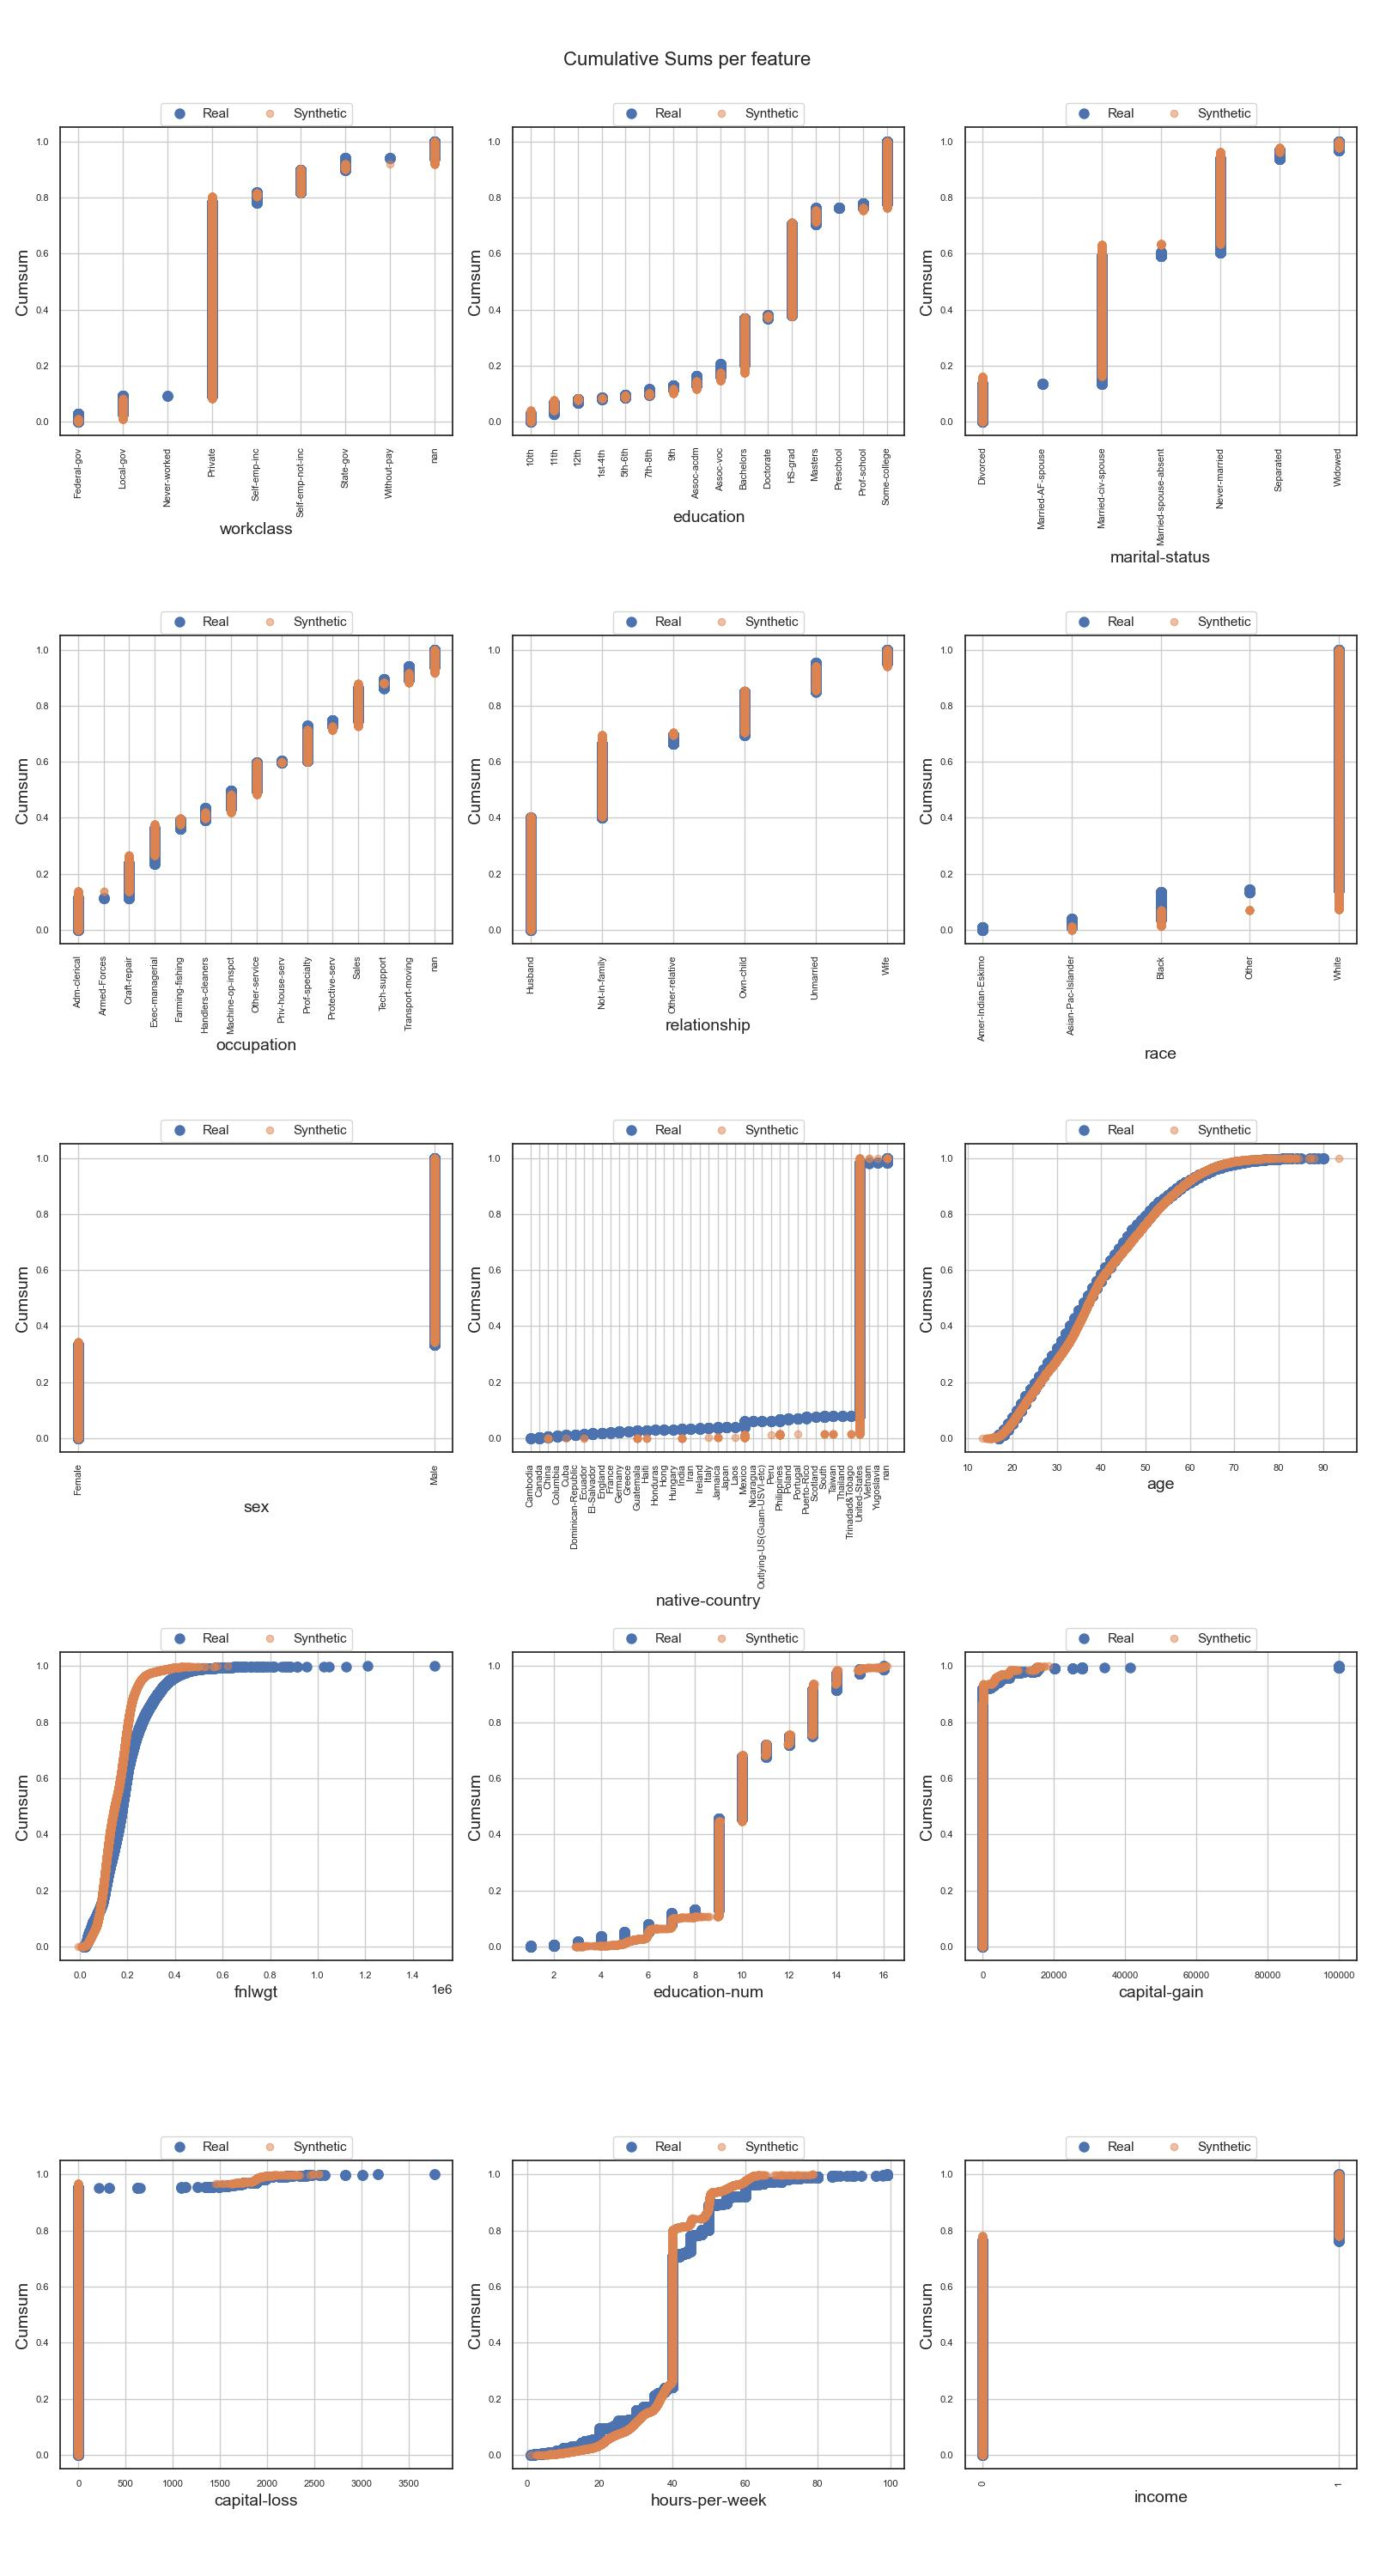
\includegraphics[height=\textheight,width=\linewidth,keepaspectratio]{images/cumsums/tvae_simTune.jpg}
			\caption{TVAE$^s$}
		\end{subfigure}
		\hfill
		\begin{subfigure}{0.3\linewidth}
			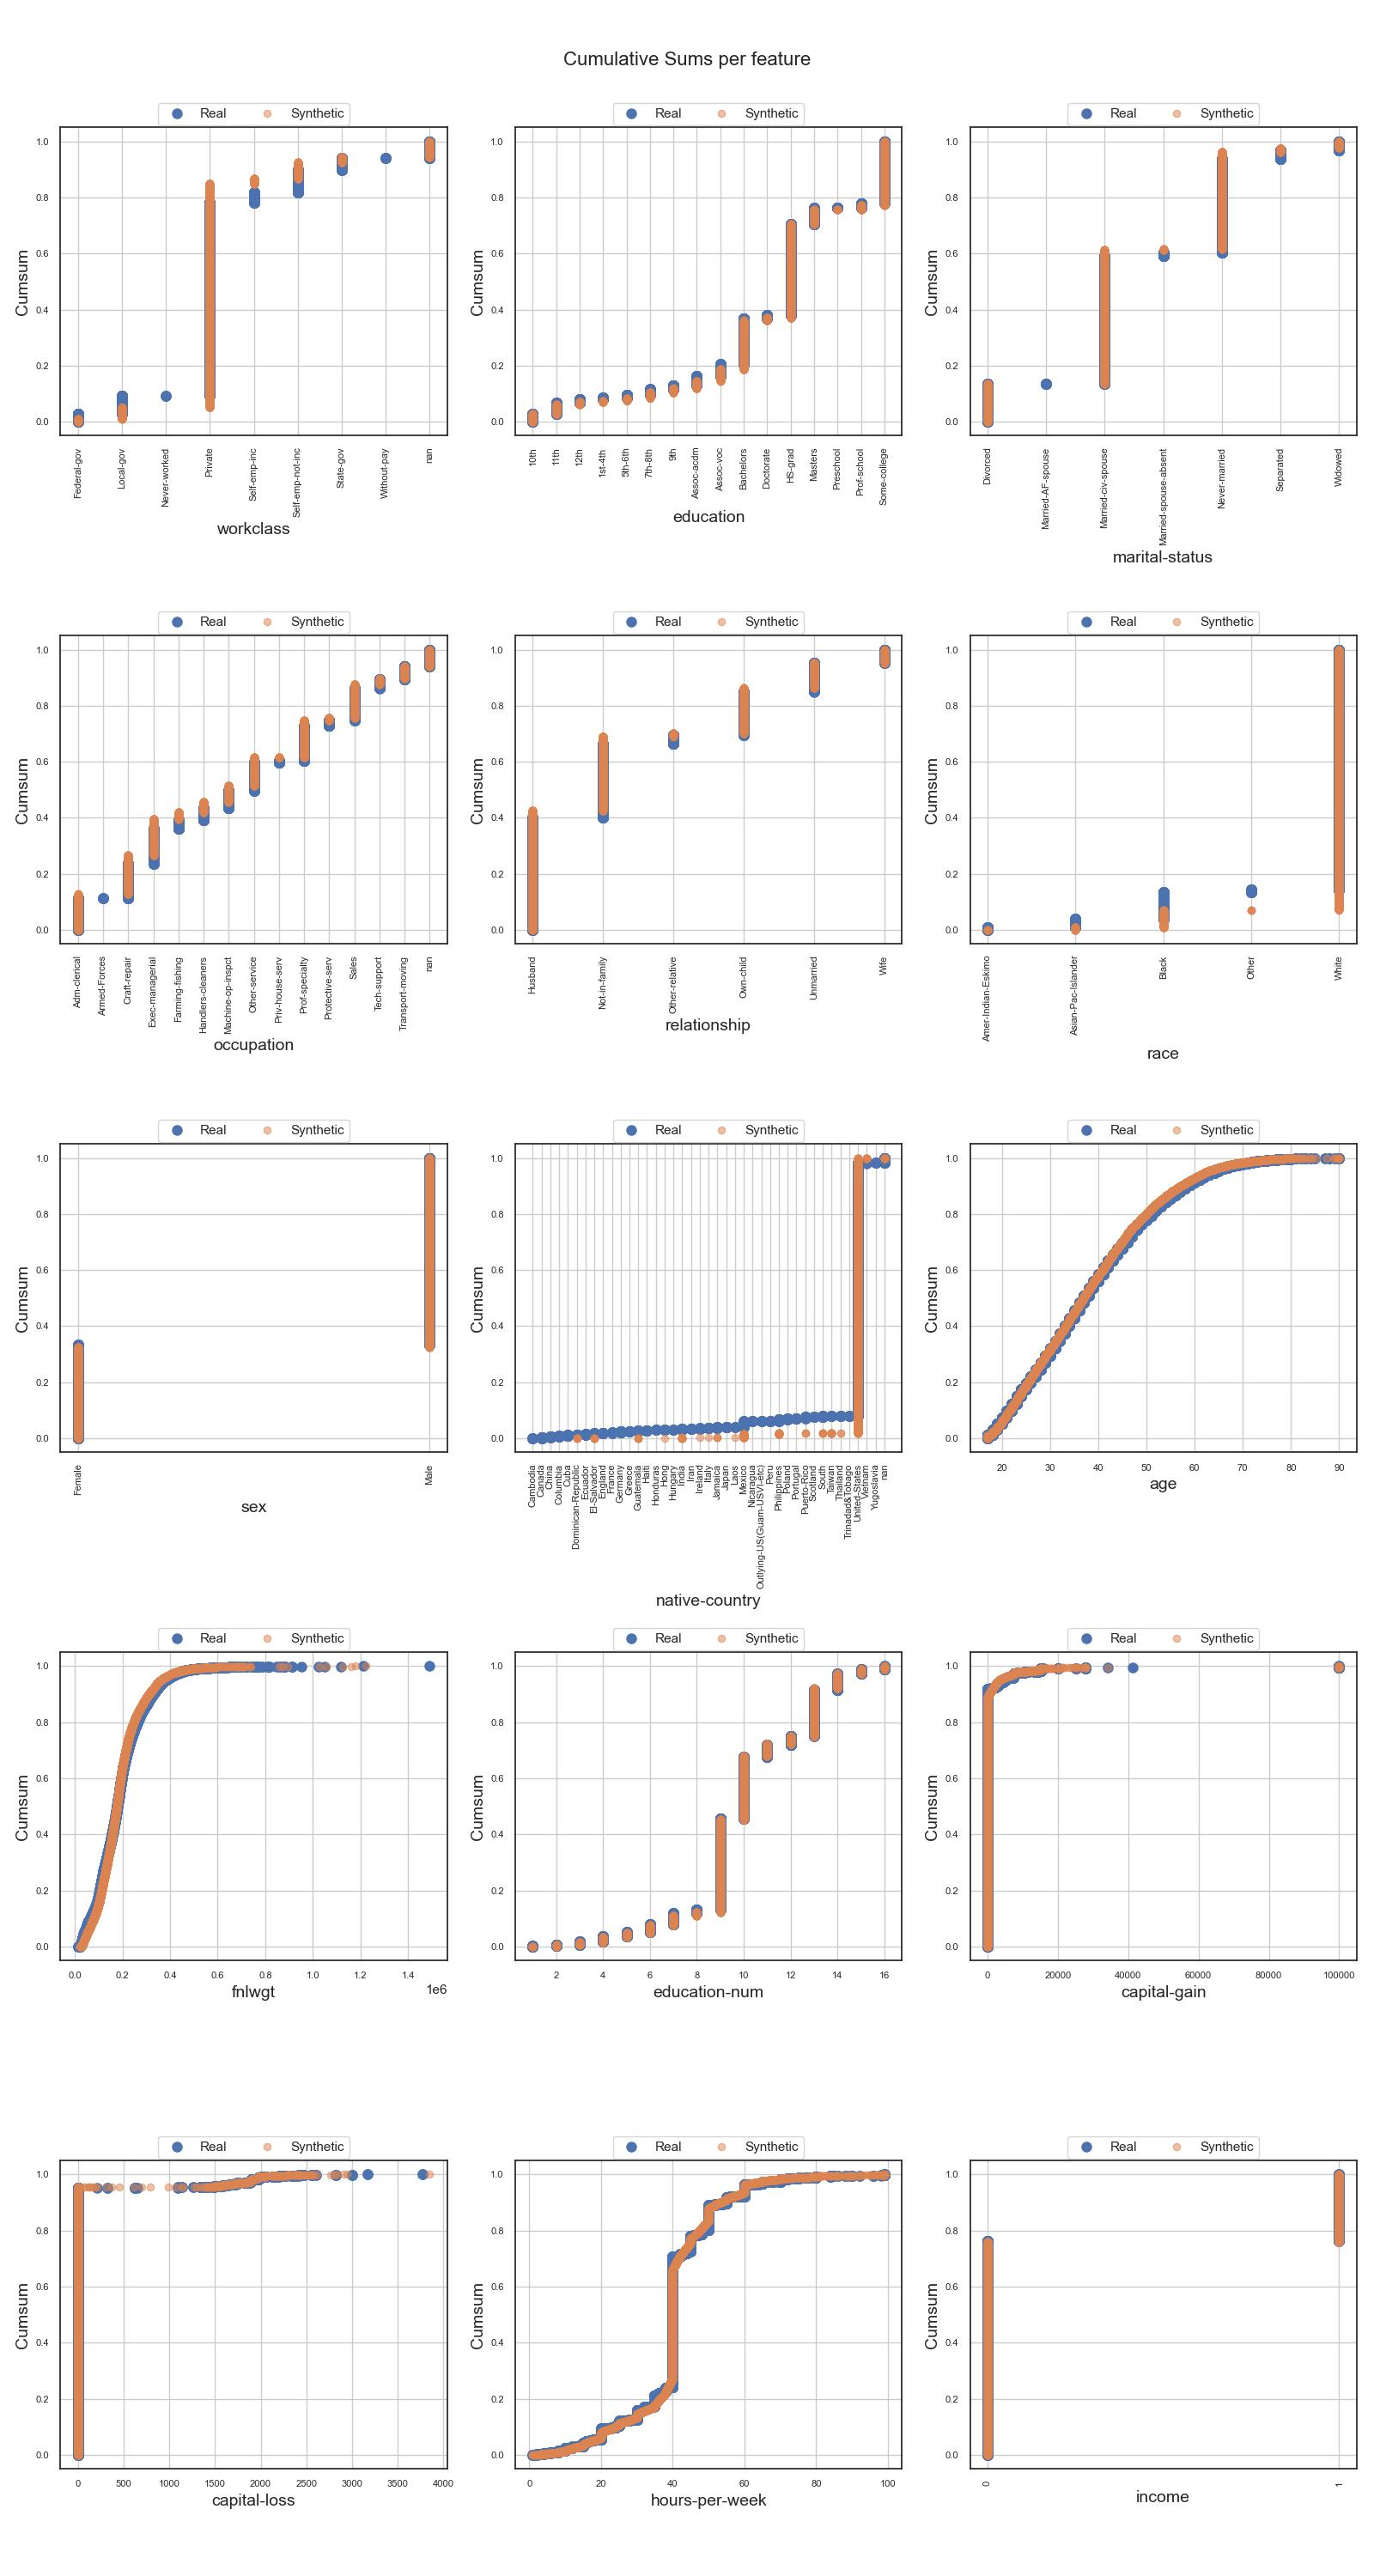
\includegraphics[height=\textheight,width=\linewidth,keepaspectratio]{images/cumsums/smote.jpg}
			\caption{SMOTE}
		\end{subfigure}
		\caption[Cumulative Distribution plots Baseline Models]{Cumulative Distribution plots for TVAE$^{ml}$, TVAE$^s$ and SMOTE}
		\label{fig_a:cumsum_2}
	\end{figure}
\end{landscape}
%----------
\newpage
\begin{landscape}
	\begin{figure}[h]
		\centering
		\hfill
		\begin{subfigure}{0.3\linewidth}
			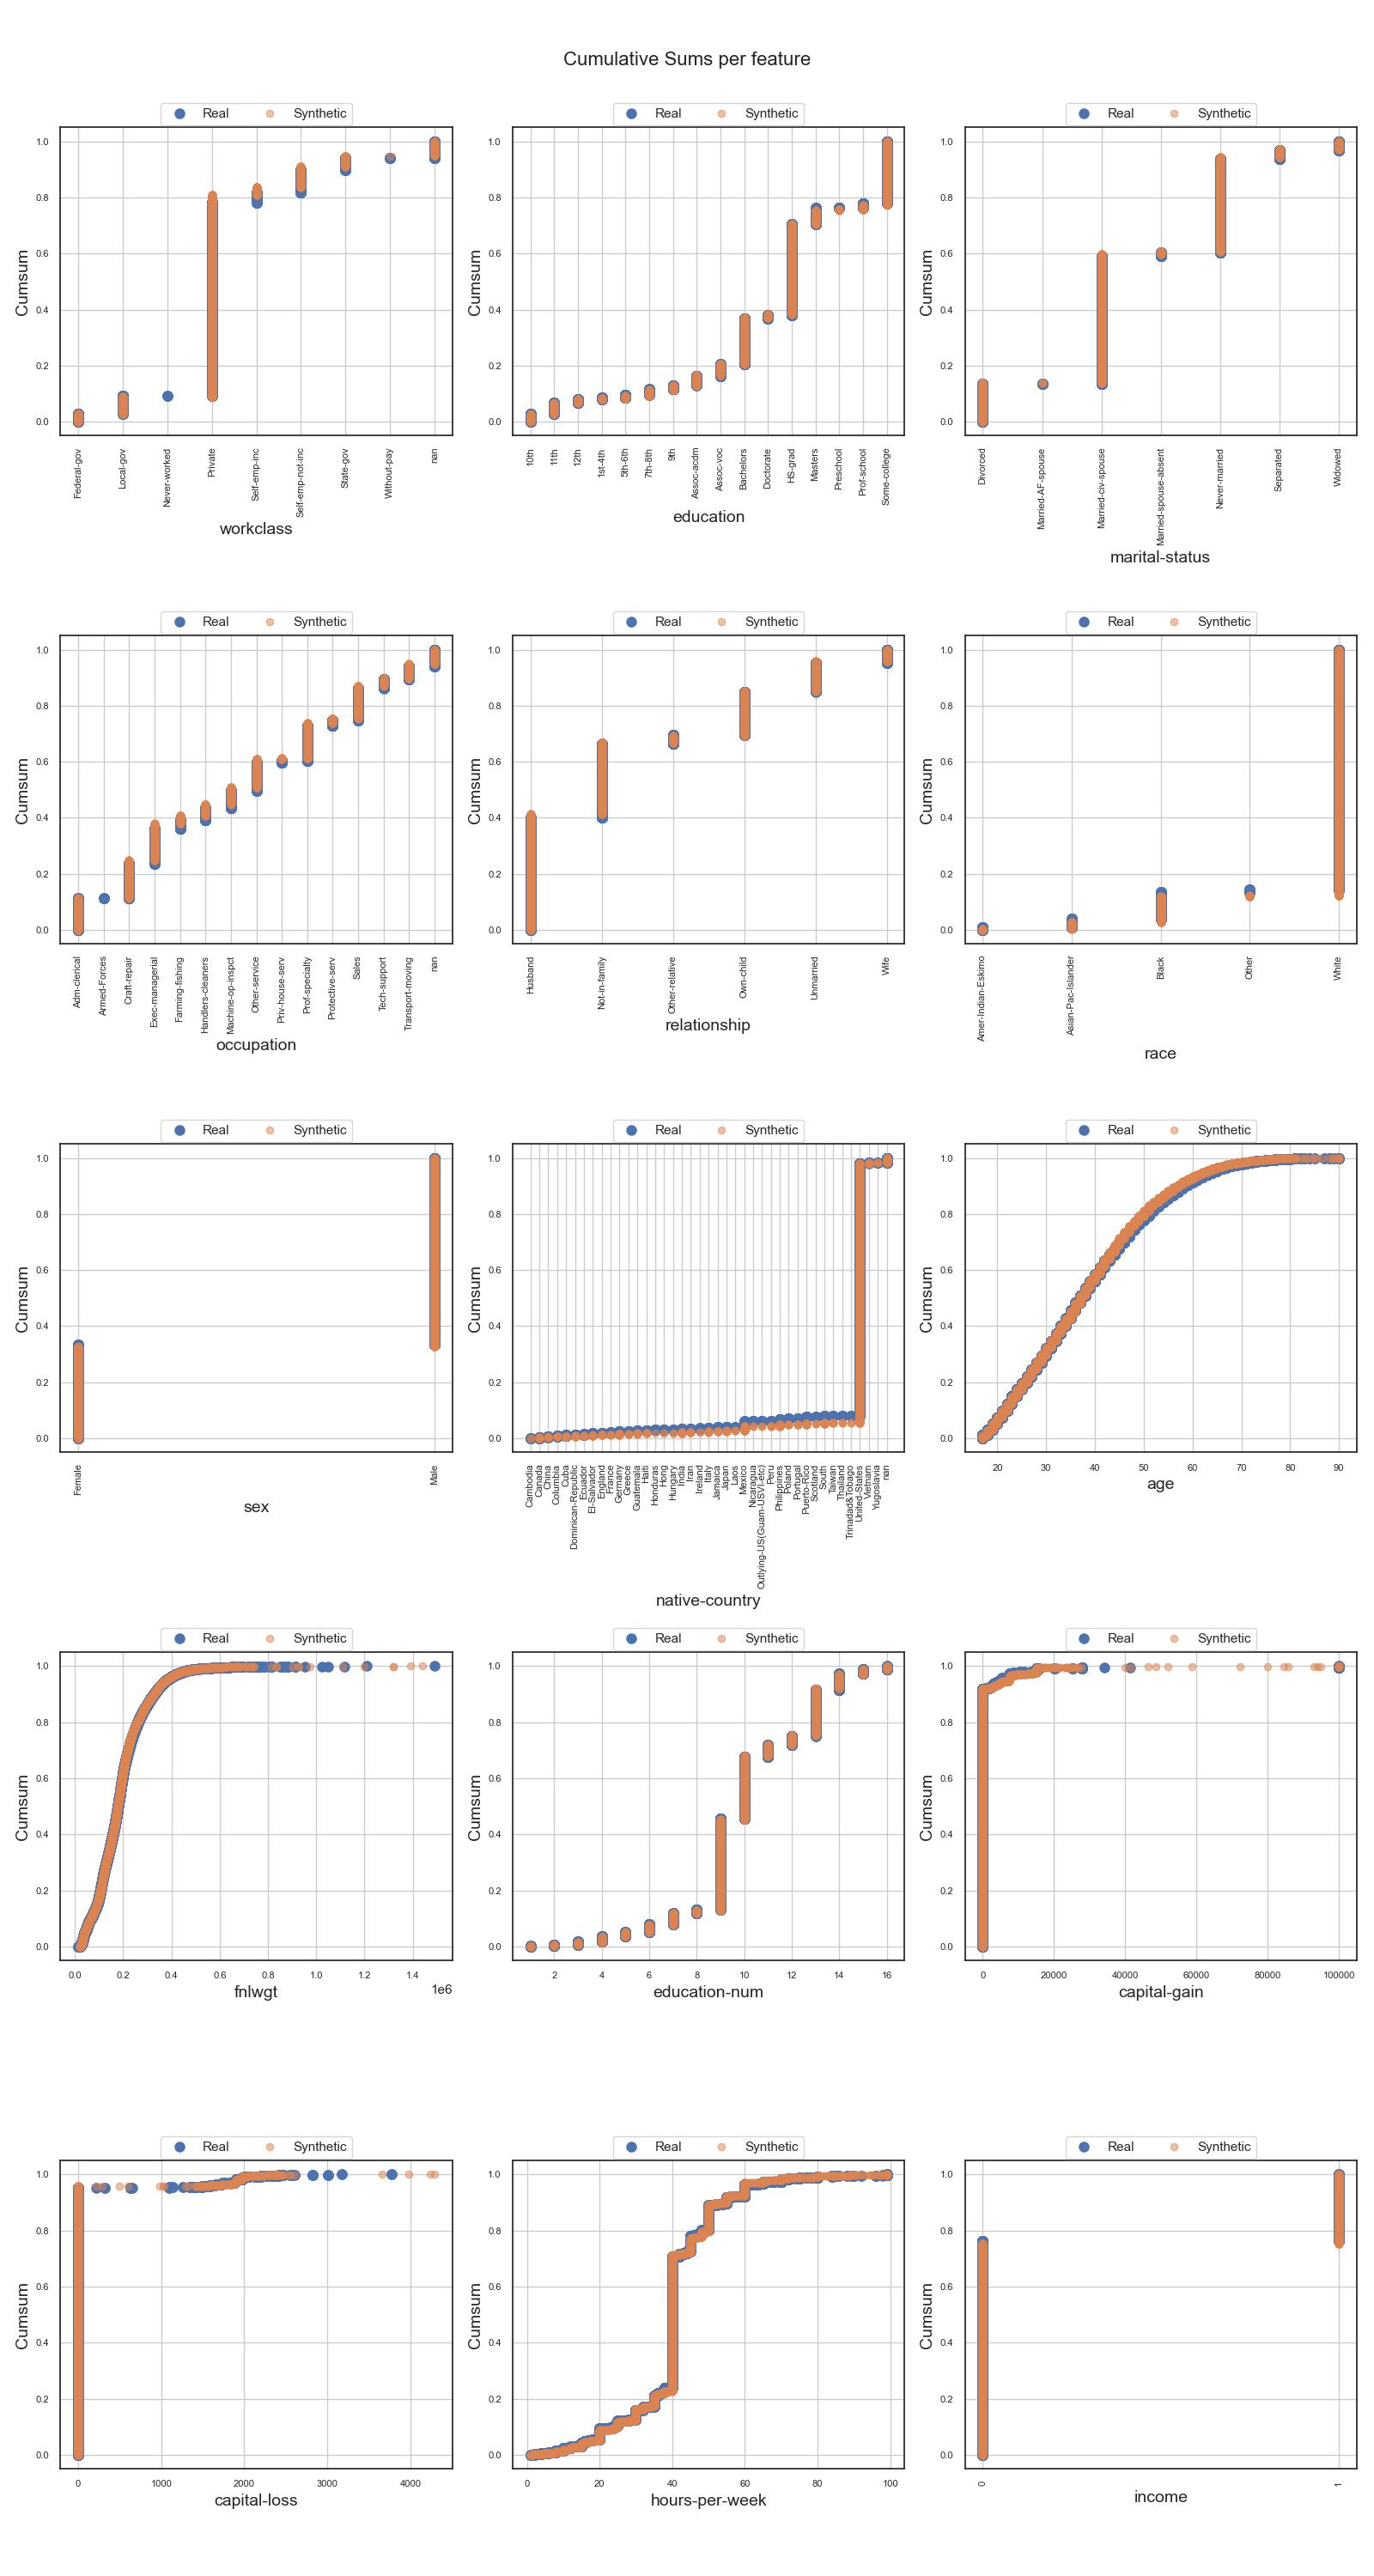
\includegraphics[height=\textheight,width=\linewidth,keepaspectratio]{images/cumsums/tab-ddpm.jpg}
			\caption{TabDDPM$^{ml}_q$}
		\end{subfigure}
		\hfill
		\begin{subfigure}{0.3\linewidth}
			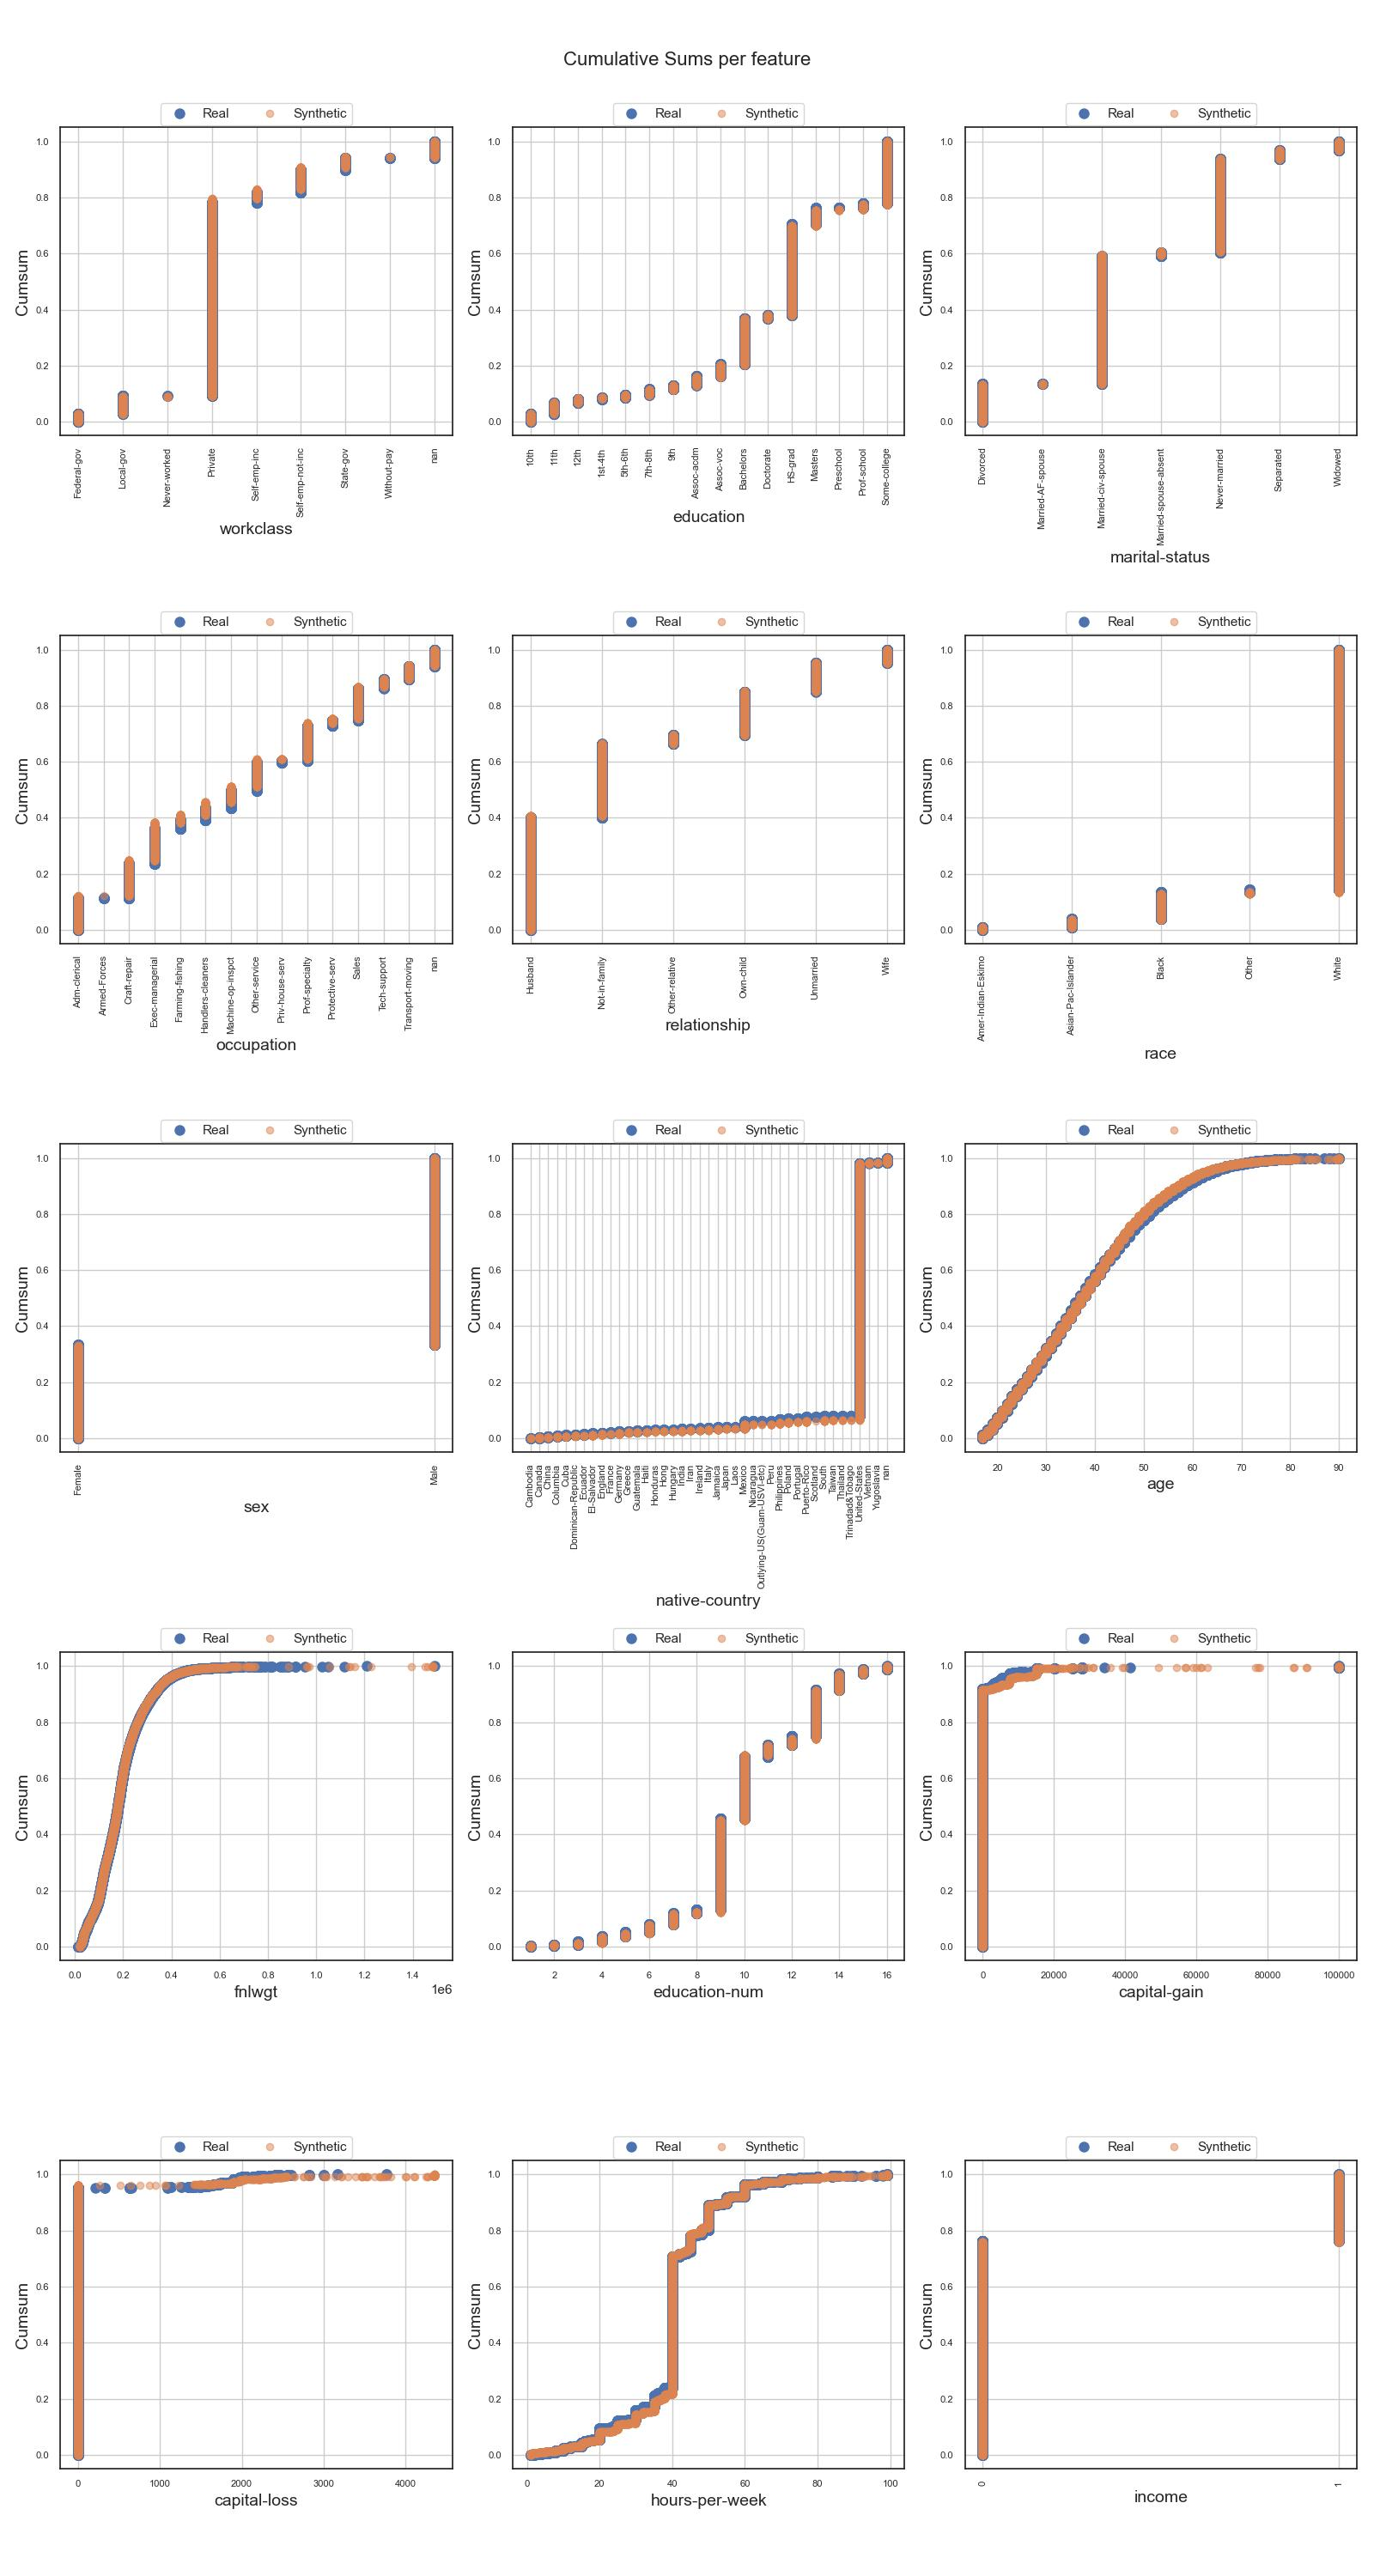
\includegraphics[height=\textheight,width=\linewidth,keepaspectratio]{images/cumsums/tab-ddpm-simTune.jpg}
			\caption{TabDDPM$^{s}_q$}
		\end{subfigure}
		\hfill
		\begin{subfigure}{0.3\linewidth}
			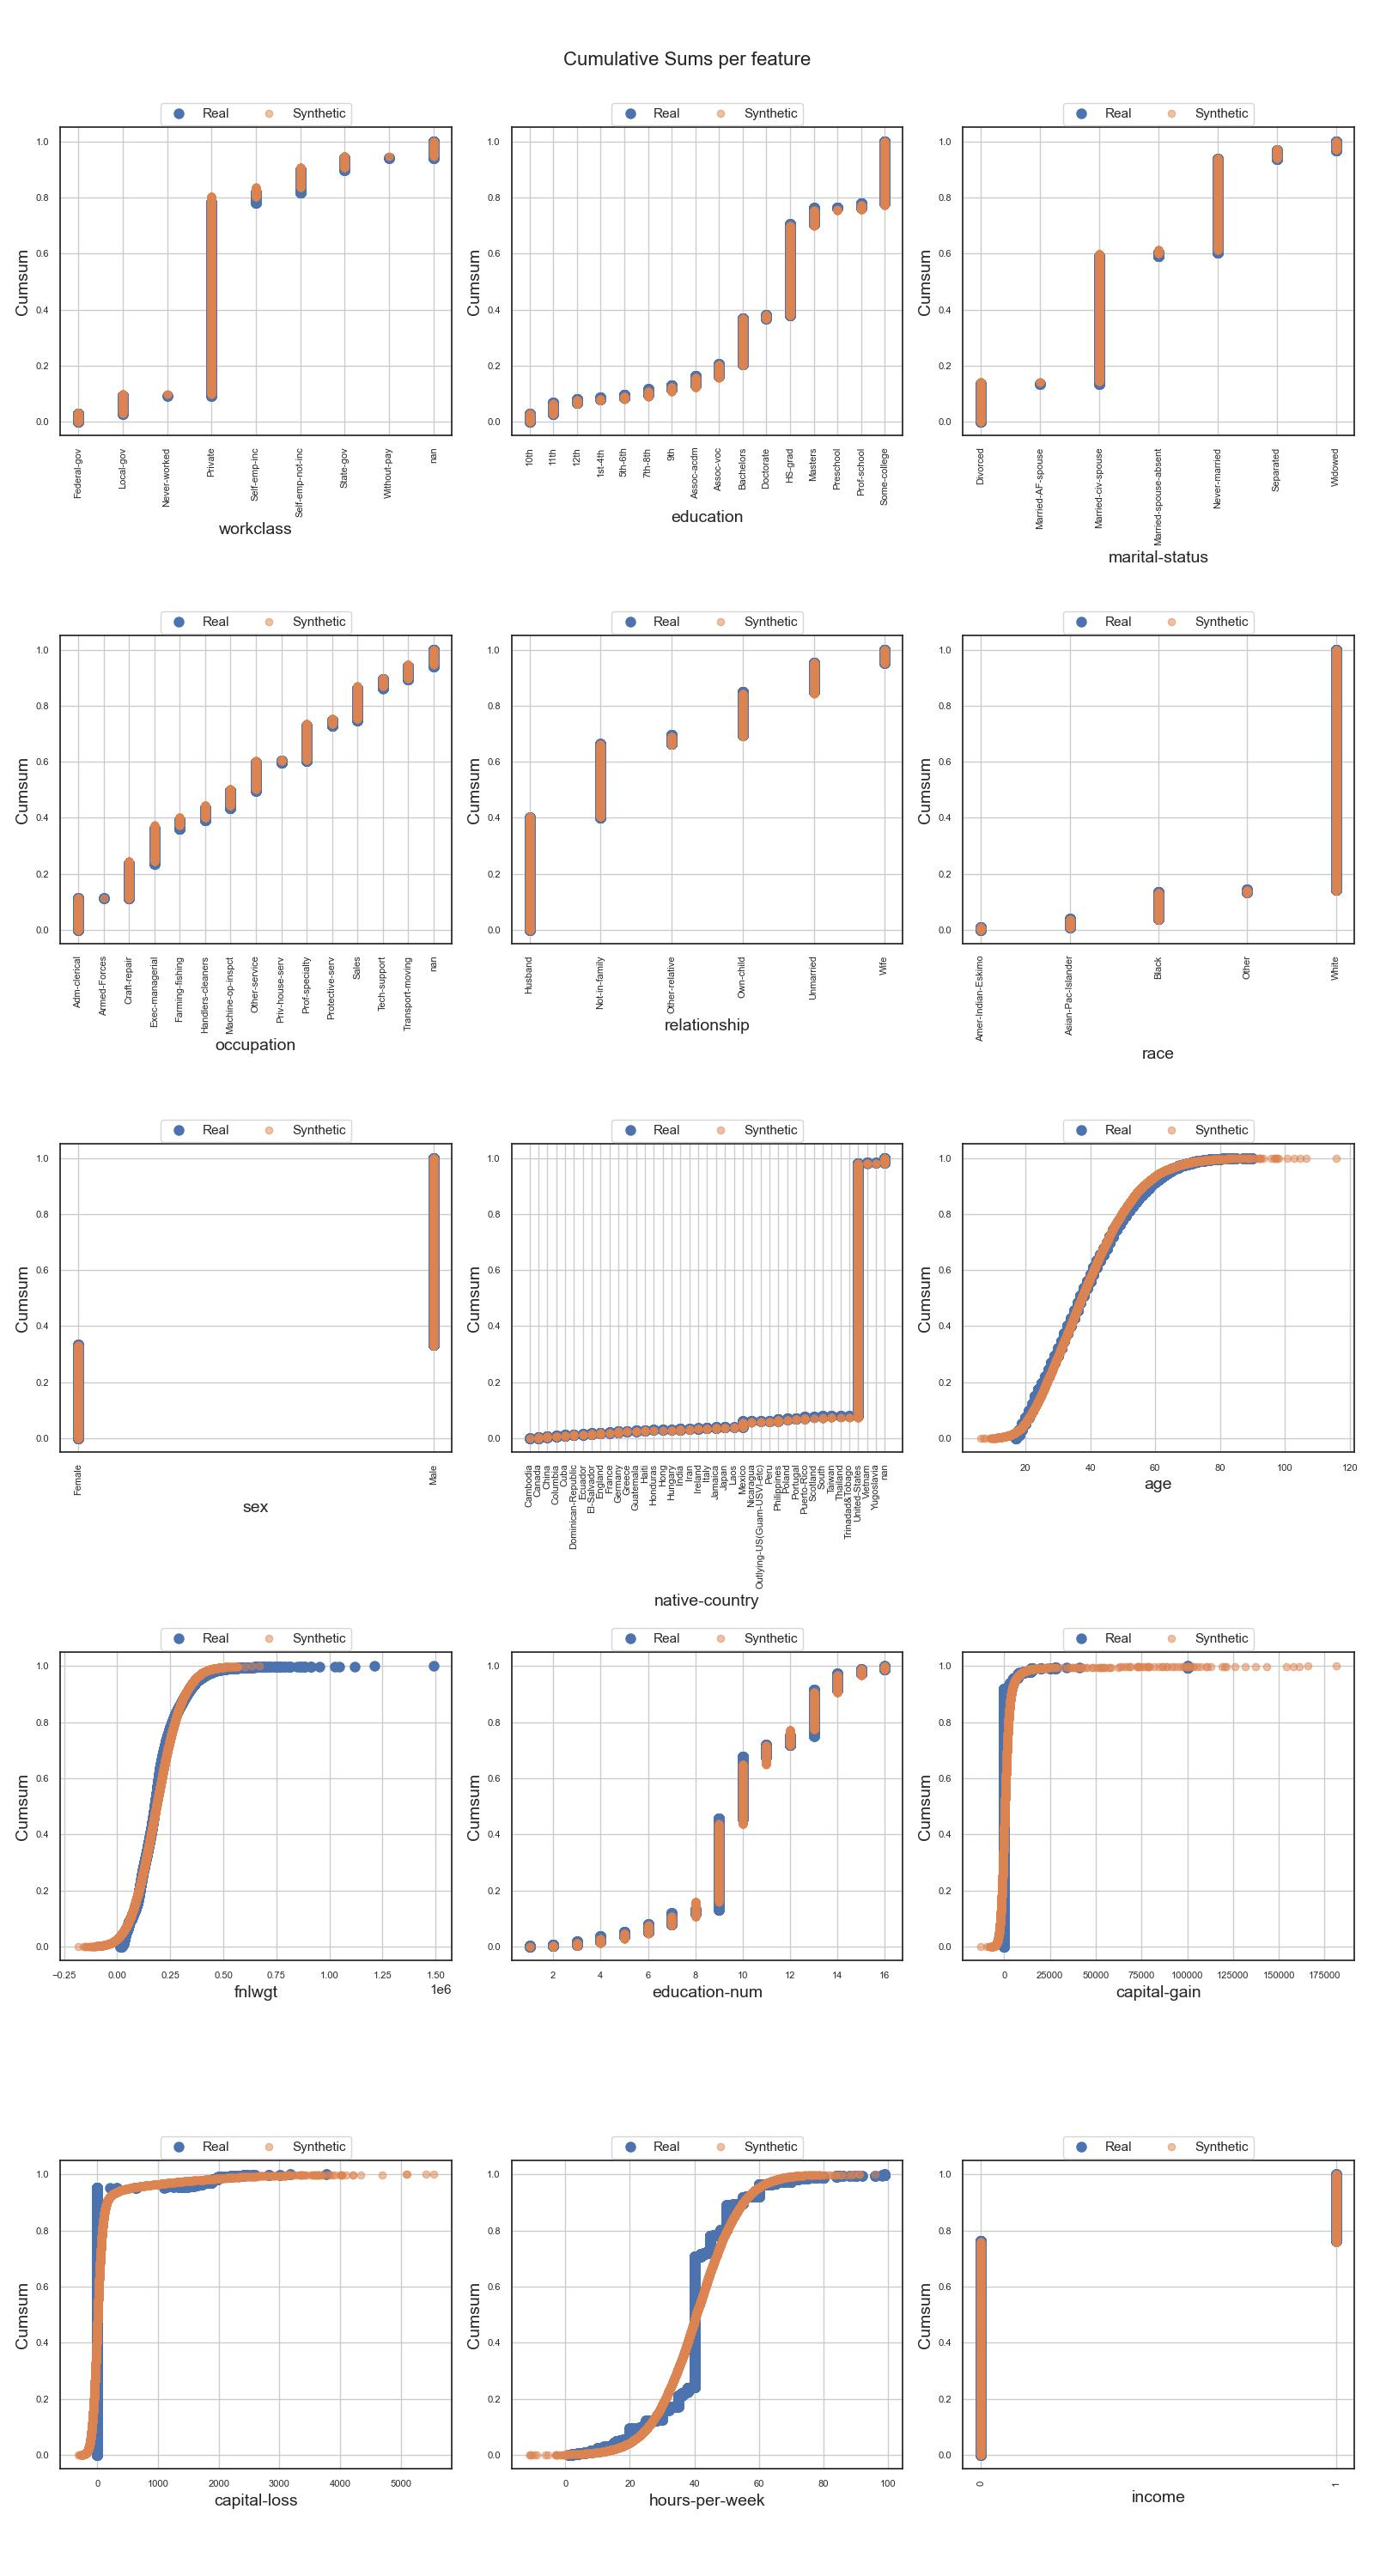
\includegraphics[height=\textheight,width=\linewidth,keepaspectratio]{images/cumsums/tab-ddpm-simTune-minmax.jpg}
			\caption{TabDDPM$^{s}_m$}
			\label{fig_a:cumsum_3_c}
		\end{subfigure}
		\hfill
		\caption[Cumulative Distribution plots TabDDPM Models]{Cumulative Distribution plots for TabDDPM variations}
		\label{fig_a:cumsum_3}
	\end{figure}
\end{landscape}
%----------
\newpage
\begin{landscape}
	\begin{figure}[h]
		\centering
		\hfill
		\begin{subfigure}{0.3\linewidth}
			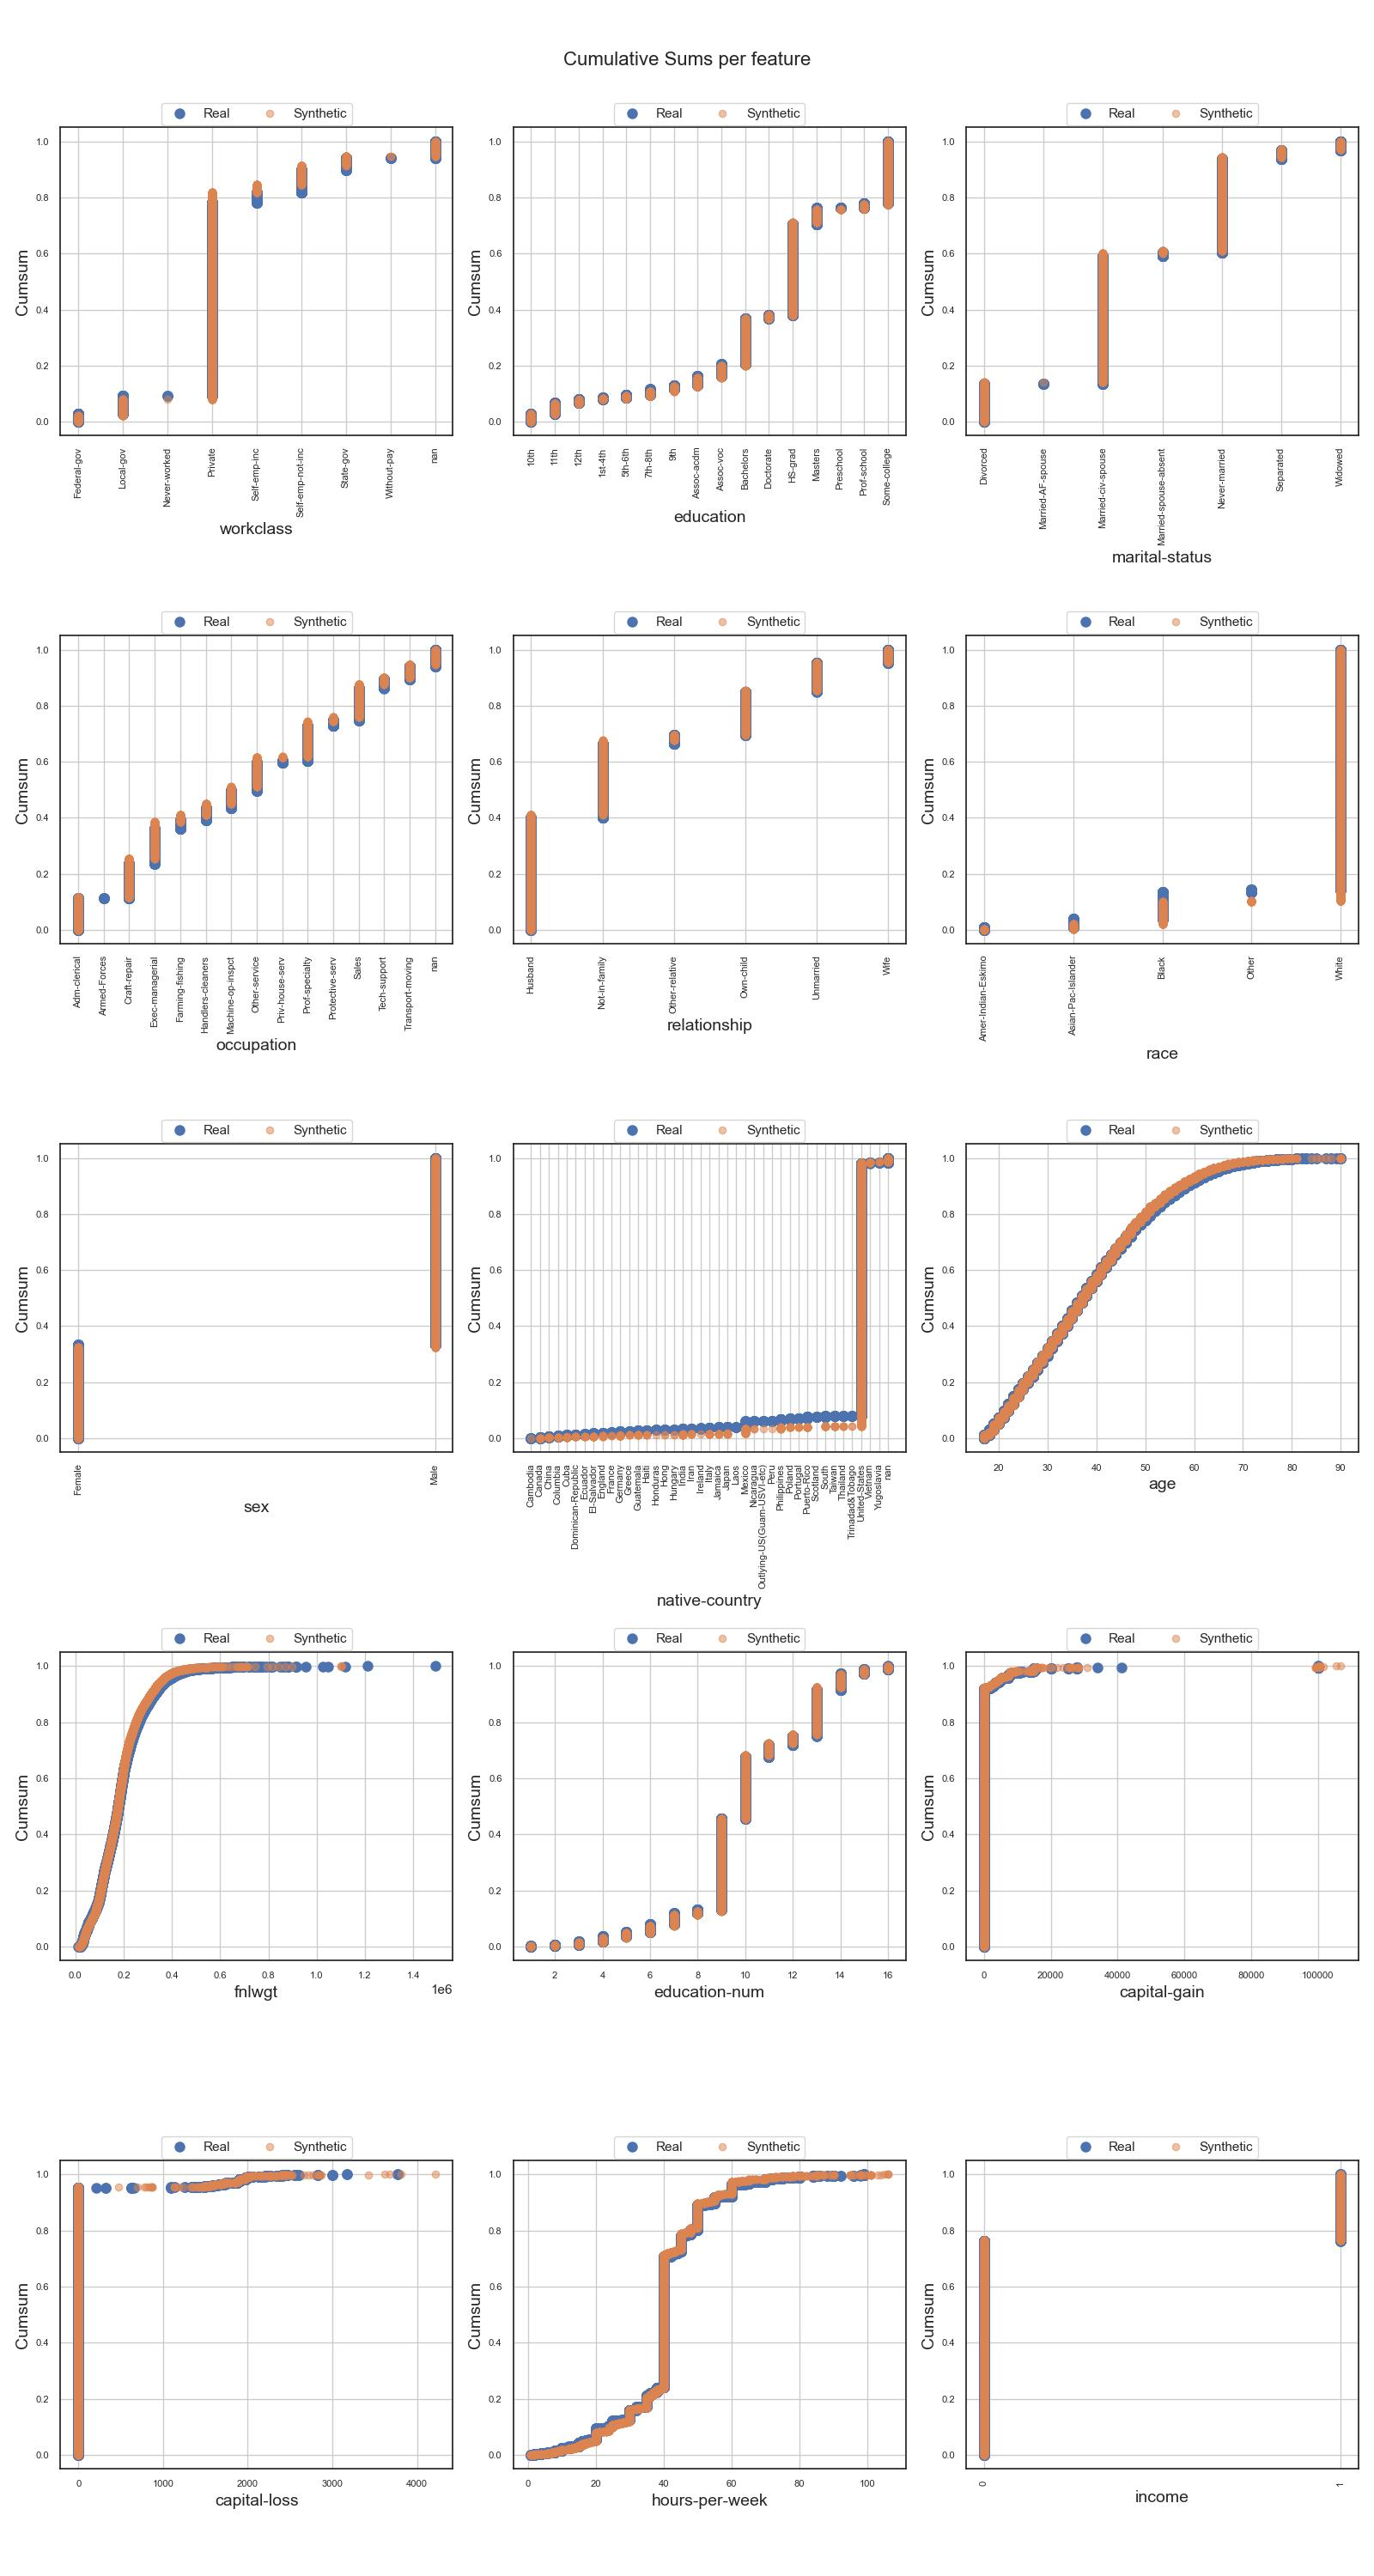
\includegraphics[height=\textheight,width=\linewidth,keepaspectratio]{images/cumsums/tab-ddpm-bgm.jpg}
			\caption{TabDDPM-BGM$^{ml}_q$}
		\end{subfigure}
		\hfill
		\begin{subfigure}{0.3\linewidth}
			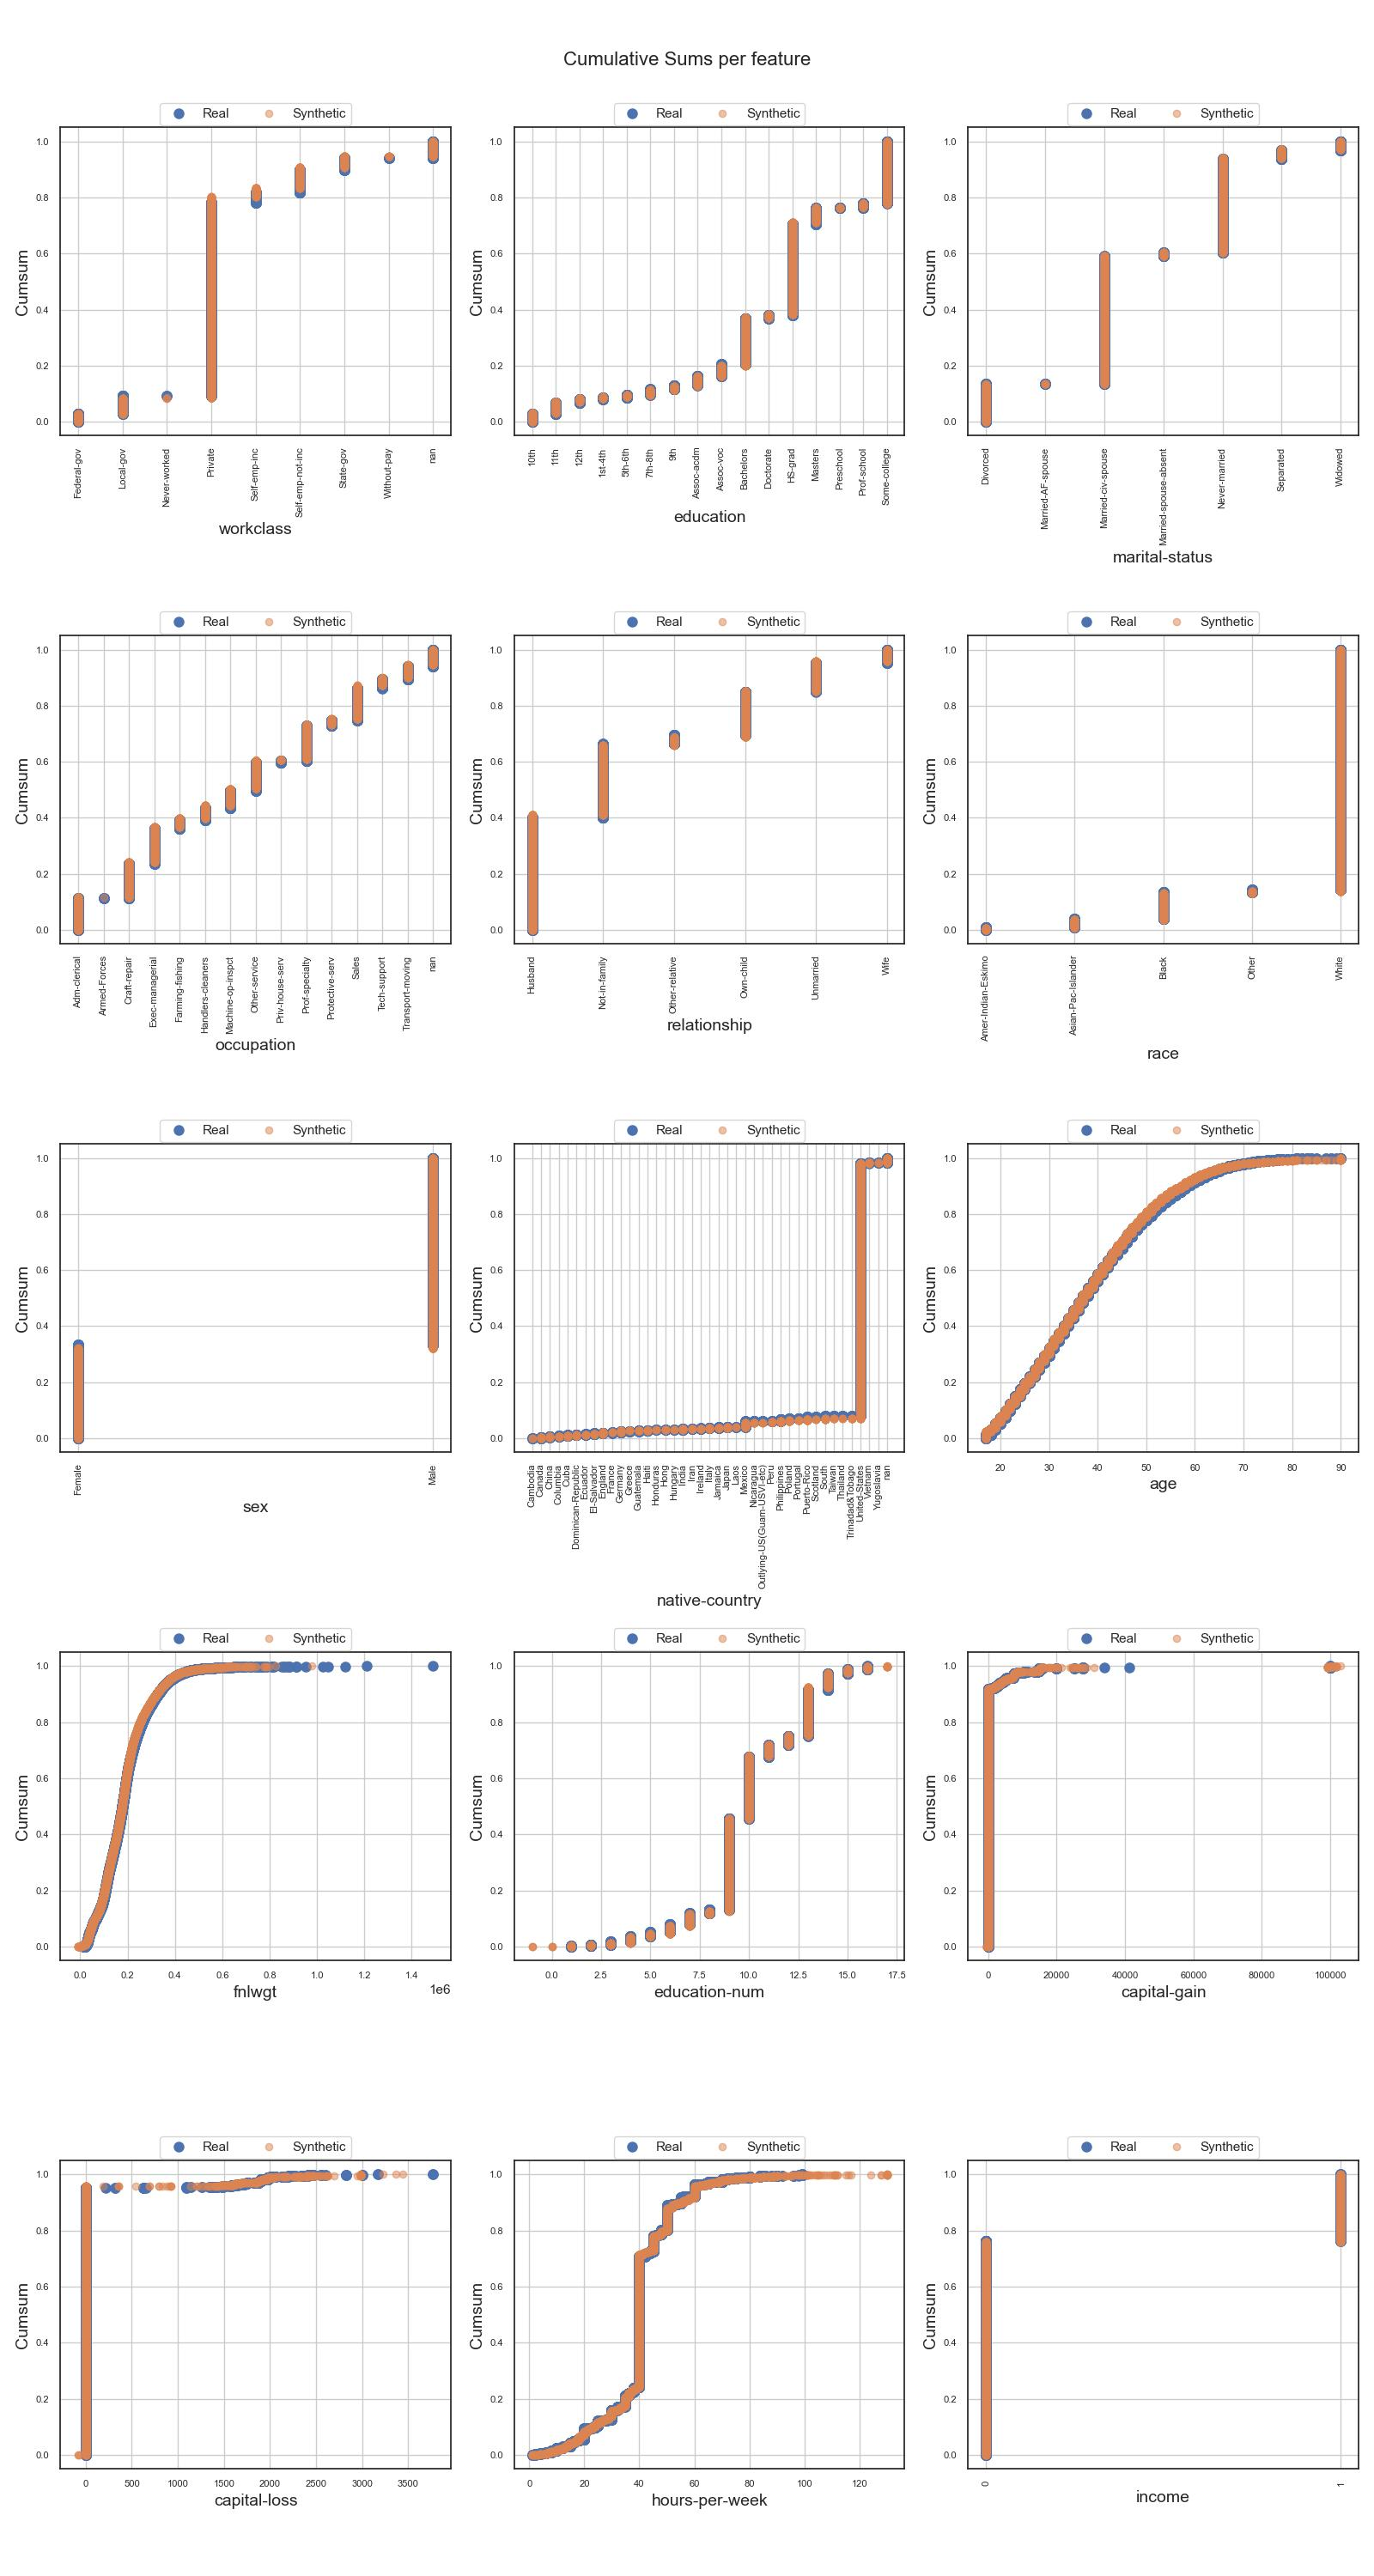
\includegraphics[height=\textheight,width=\linewidth,keepaspectratio]{images/cumsums/tab-ddpm-bgm-simTune.jpg}
			\caption{TabDDPM-BGM$^{s}_q$}
		\end{subfigure}
		\hfill
		\begin{subfigure}{0.3\linewidth}
			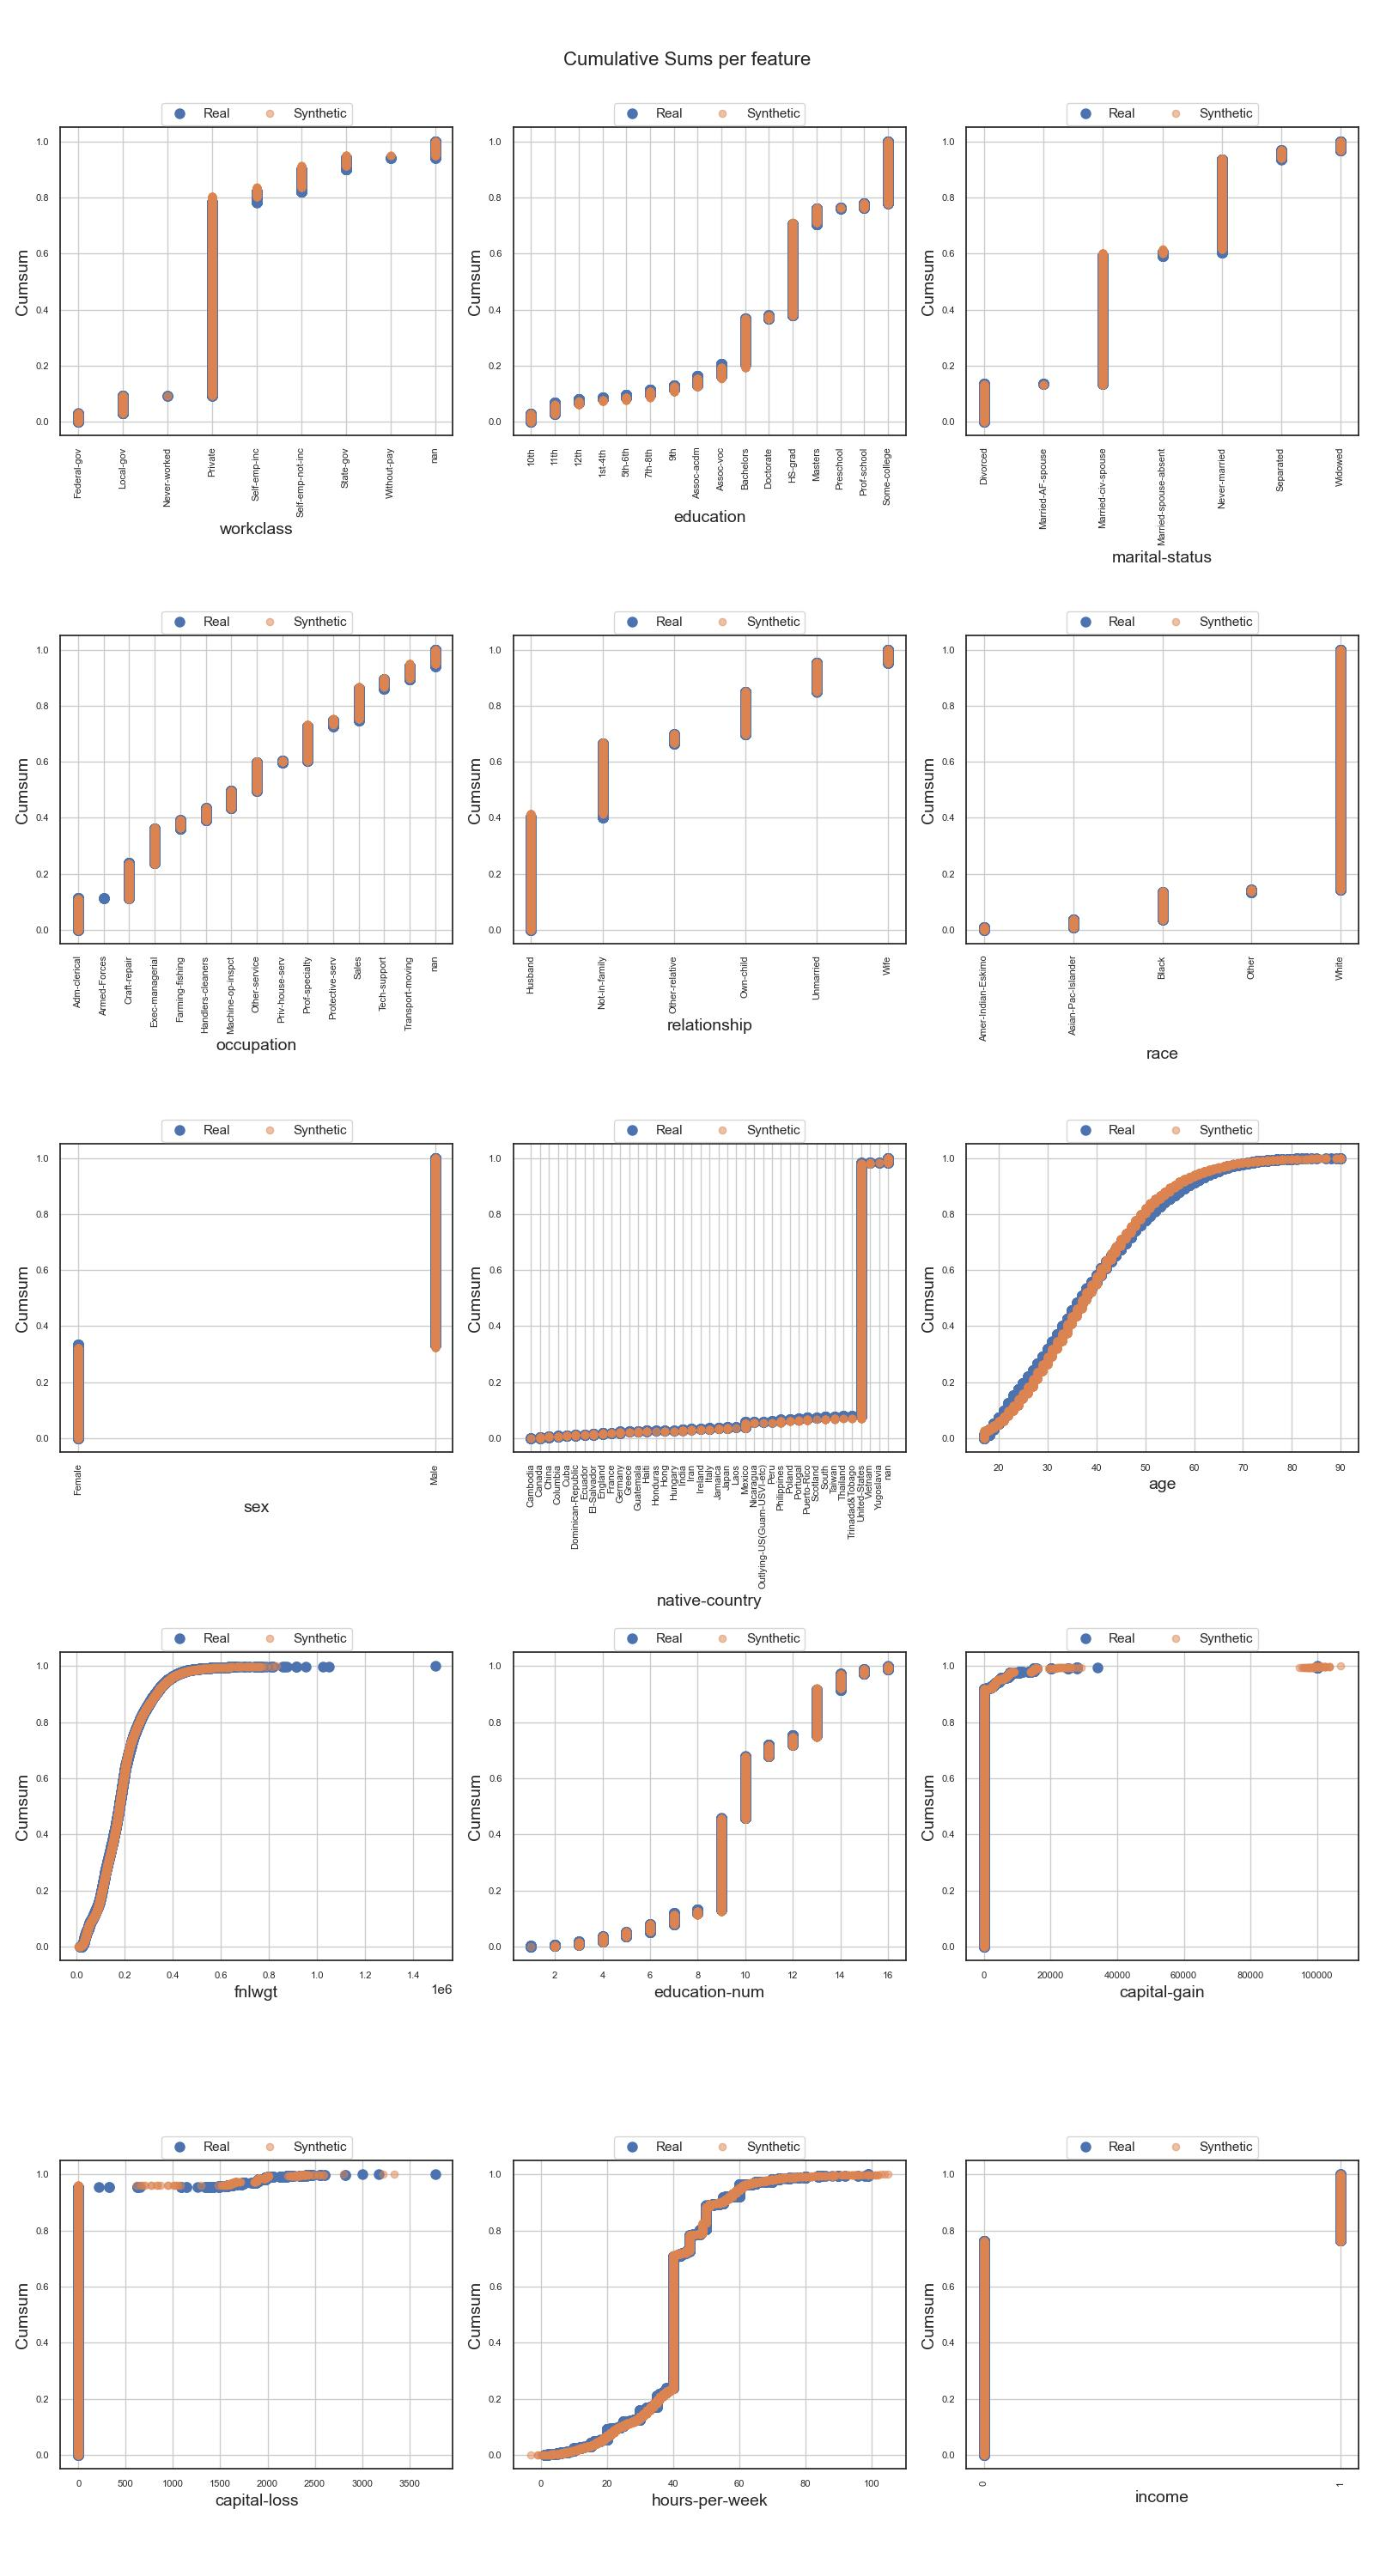
\includegraphics[height=\textheight,width=\linewidth,keepaspectratio]{images/cumsums/tab-ddpm-bgm-simTune-minmax.jpg}
			\caption{TabDDPM-BGM$^{s}_m$}
		\end{subfigure}
		\caption[Cumulative Distribution plots TabDDPM-BGM Models]{Cumulative Distribution plots for TabDDPM-BGM variations}
		\label{fig_a:cumsum_4}
	\end{figure}
\end{landscape}
%----------
\newpage
\begin{landscape}
	\begin{figure}[h]
		\centering
		\hfill
		\begin{subfigure}{0.3\linewidth}
			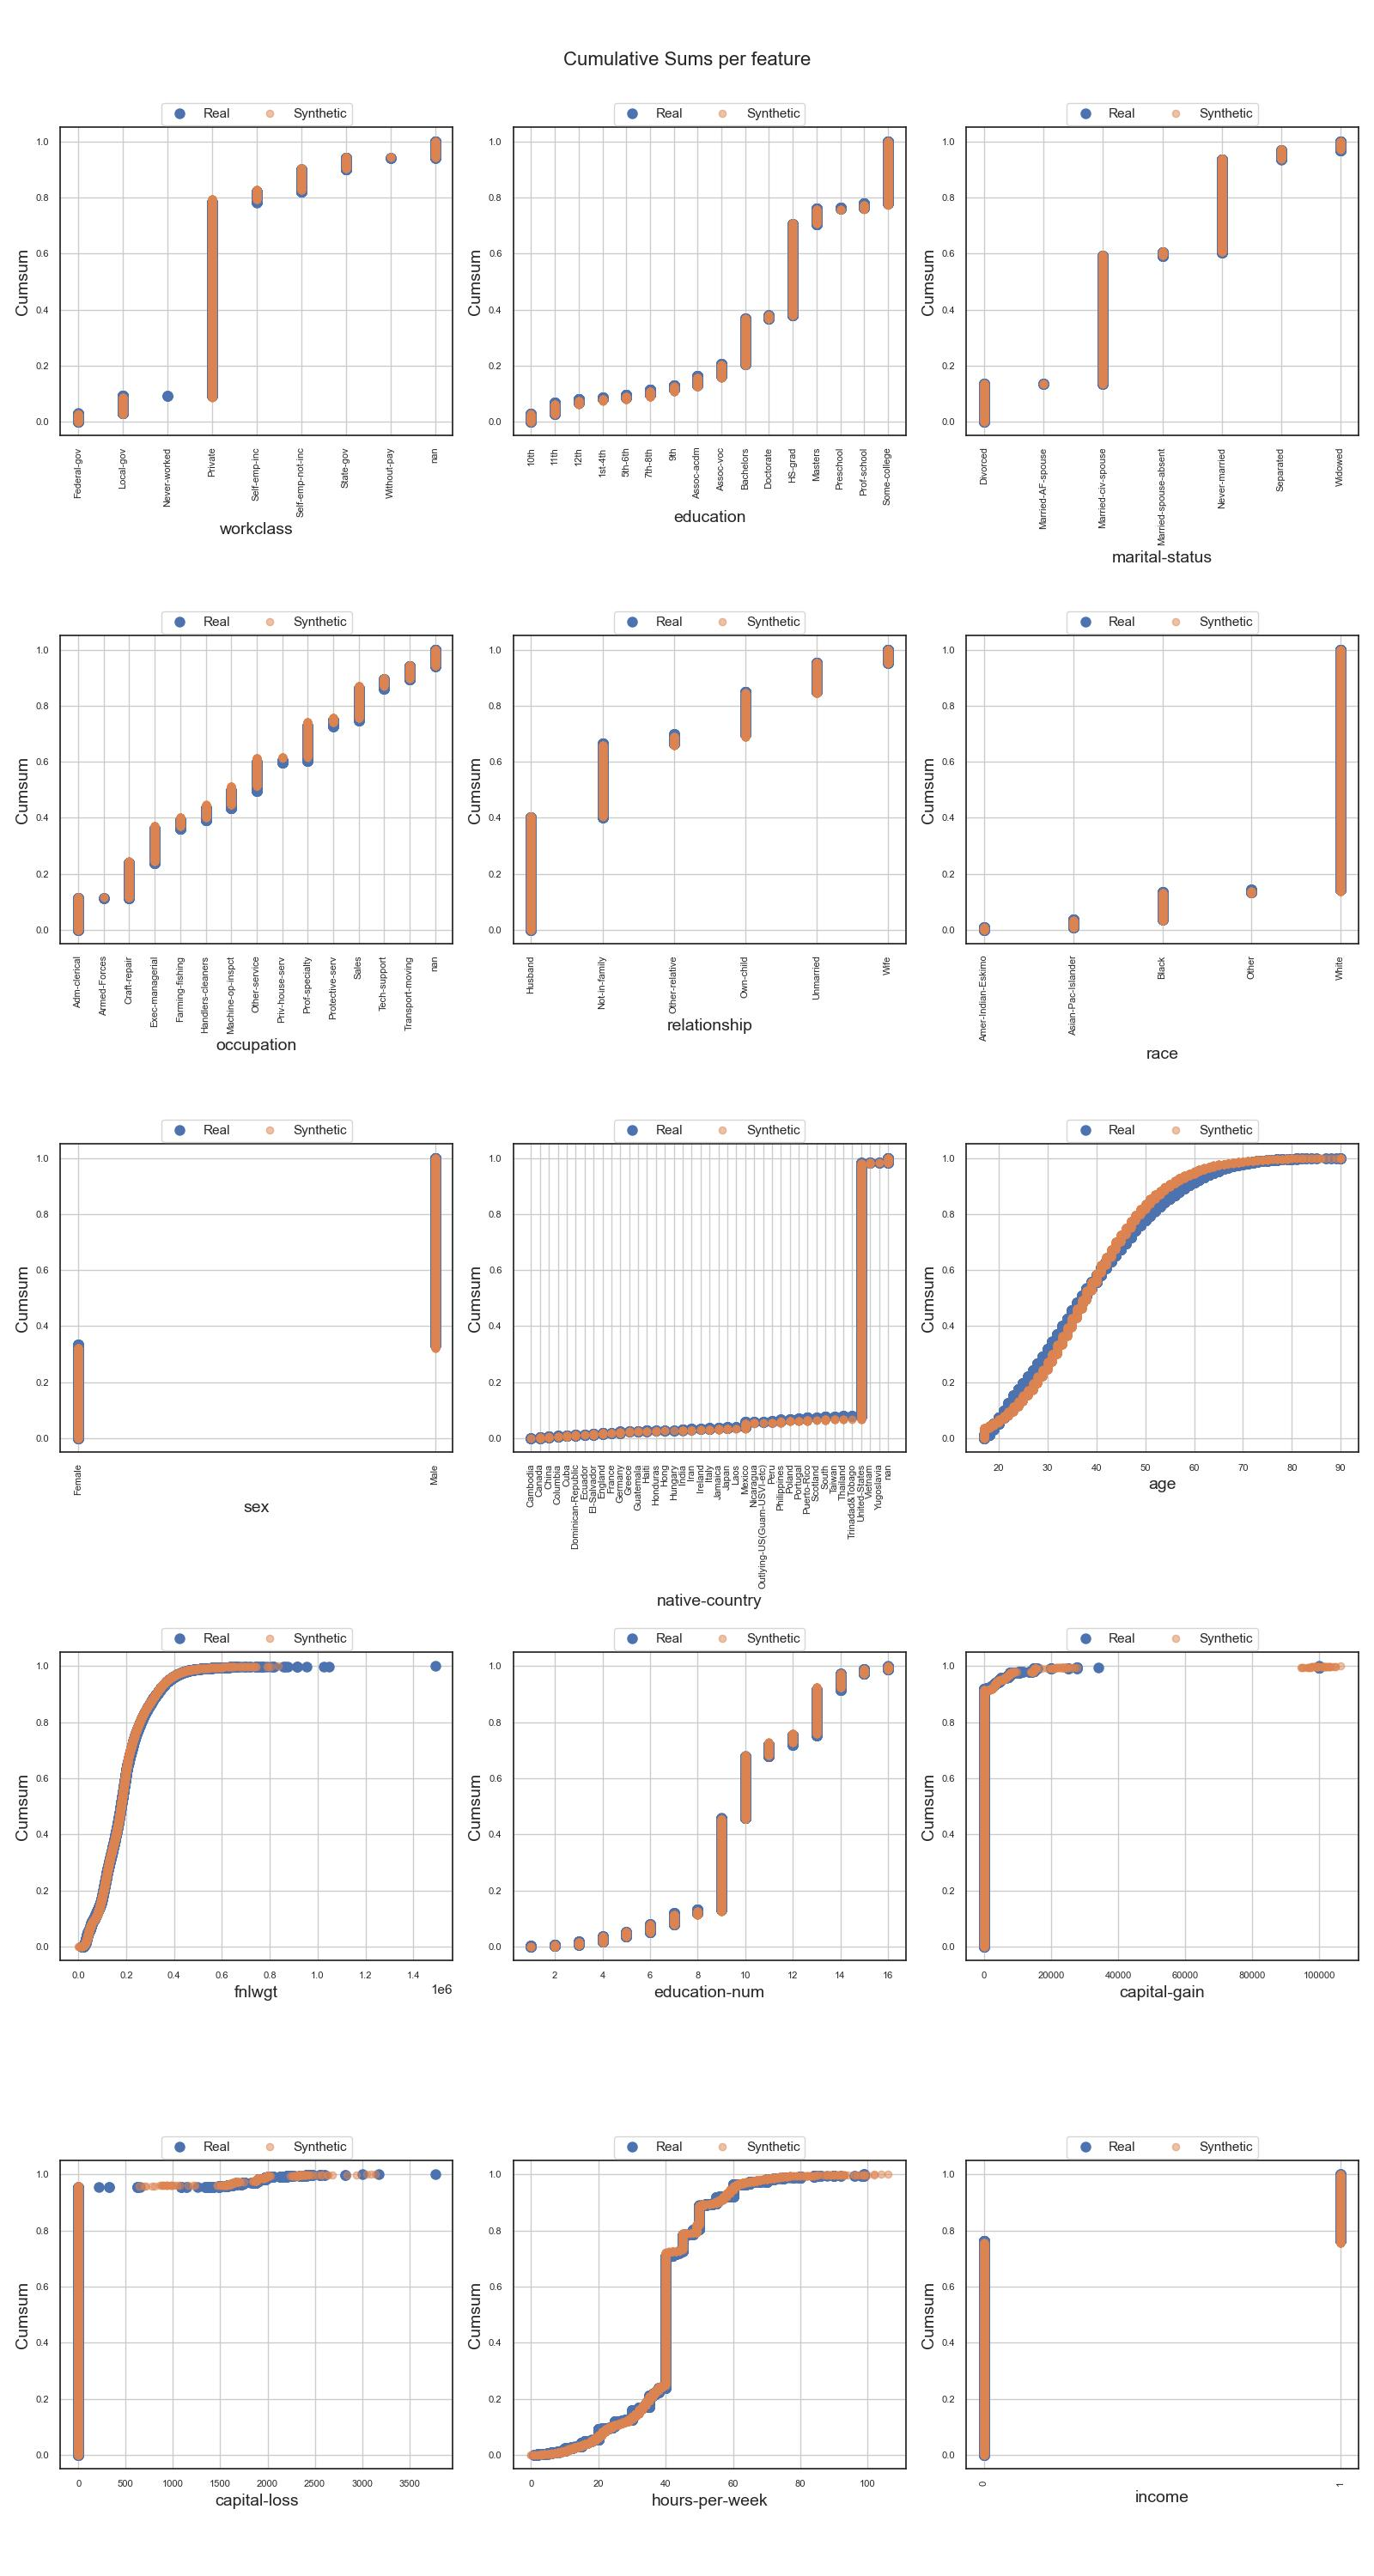
\includegraphics[height=\textheight,width=\linewidth,keepaspectratio]{images/cumsums/tab-ddpm-bgm-simTune-none.jpg}
			\caption{TabDDPM-BGM$^{s}_n$}
		\end{subfigure}
		\hfill
		\begin{subfigure}{0.3\linewidth}
			\includegraphics[height=\textheight,width=\linewidth,keepaspectratio]{images/cumsums/tab-ddpm-ft.jpg}
			\caption{TabDDPM-FT$^{ml}_q$}
		\end{subfigure}
		\hfill
		\begin{subfigure}{0.3\linewidth}
			\includegraphics[height=\textheight,width=\linewidth,keepaspectratio]{images/cumsums/tab-ddpm-ft-simTune.jpg}
			\caption{TabDDPM-FT$^{ml}_q$}
		\end{subfigure}
		\caption[Cumulative Distribution plots TabDDPM-FT Models]{Cumulative Distribution plots for TabDDPM-FT variations}
		\label{fig_a:cumsum_5}
	\end{figure}
\end{landscape}




